\documentclass[preprint,12pt]{elsarticle}

\usepackage{standalone}
\usepackage{import}
\usepackage{pgfplots}
% \usepackage{color}
\usepackage{tikz}
\usepackage{pgfplots}
\usepgfplotslibrary{fillbetween}
\pgfplotsset{compat=1.16}
\usetikzlibrary {arrows.meta, automata, positioning, fit}
\usepackage{url}
\usepackage{algorithm}
\usepackage{algpseudocode}
\usepackage{amsfonts}
\usepackage{amsmath, amssymb, amsthm}
\usepackage{float, subcaption, graphics}
\usepackage{mathbbol}
\usepackage{colortbl}
\definecolor{grayshade}{gray}{0.9}
\usepackage{array} % Required for custom column formatting
\usepackage[normalem]{ulem} % Required for delete line on text. The usage is : \sout{Hello World}
\usepackage{hyperref} % Required for URL. The usage is : \url{www.helloworld.com}
\usepackage{microtype}

\hypersetup{
    colorlinks=true,
    linkcolor=blue,
    filecolor=magenta,      
    urlcolor=cyan,
    pdftitle={Overleaf Example},
    pdfpagemode=FullScreen,
    }

\captionsetup[table]{skip=10pt} %


% set algorithmicx
\renewcommand{\algorithmicrequire}{\textbf{Input:}}  % Use Input in the format of Algorithm  
\renewcommand{\algorithmicensure}{\textbf{Output:}} % Use Output in the format of Algorithm   

\newcommand*{\Int}{\mathbb{Z}}
\newcommand*{\Nat}{\mathbb{N}}
\newcommand*{\NFA}{\mathcal{A}}
\newcommand{\Lang}{\mathcal{L}}
\newcommand{\cefaout}{\mathcal{O}}
\newcommand*{\op}{o}
\newcommand*{\svars}{{\sf SVars}}
\newcommand*{\ivars}{{\sf IVars}}

\newcommand{\anivar}{\mathfrak{x}}
\newcommand{\anivary}{\mathfrak{y}}
\newcommand{\anivarz}{\mathfrak{z}}

\newtheorem*{proof*}{Proof}
\newtheorem{lemma}{Lemma}
\newtheorem{theorem}{Theorem}
\newtheorem{definition}{Definition}
\newtheorem{proposition}{Proposition}
\newtheorem{example}{Example}
\newtheorem{observation}{Observation}

\newcommand*{\prj}{{\sf prj}}

\newcommand*{\red}[1]{\textcolor{red}{#1}}

\newcommand{\costset}{\mathbb{C}}
\newcommand{\confset}{\mathsf{Conf}}

\newcommand*{\myvec}[1]{\vec{#1}}
\newcommand*{\regex}{e}
\newcommand*{\strsort}{\verb|Str|}
\newcommand*{\intsort}{\verb|Int|}
\newcommand*{\lan}{\mathcal{L}}
\newcommand*{\highlight}[1]{\textbf{\textit{#1}}}
\newcommand*{\aut}{\mathcal{A}}
\newcommand*{\algfun}[1]{\texttt{#1}}
\newcommand*{\strlen}[1]{\texttt{len}(#1)}
\newcommand*{\myemph}[1]{\textcolor{red}{#1}}
\newcommand*{\mult}[1]{$\times$}
\newcommand*{\ostrichrecl}{\rm OSTRICH^{RECL}}
\newcommand*{\emptinessprob}{$SAT_{CEFA}[LIA]$ problem}

\newcommand{\srel}{\mathsf{Rel}}

\newcommand{\ltrue}{\mathtt{true}}
\newcommand{\lfalse}{\mathtt{false}}
%%
\newcommand{\hide}[1]{ }

\newcommand{\cB}{\mathcal{B}}
\newcommand{\cC}{\mathcal{C}}
\newcommand{\cD}{\mathcal{D}}
\newcommand{\amodel}{\mathfrak{m}}
\newcommand{\nvec}{\mathfrak{n}}
\newcommand{\cT}{\mathcal{T}}
\newcommand{\cU}{\mathcal{U}}
\newcommand{\fZ}{\mathfrak{Z}}

\newcommand{\concat}{\cdot}

\newcommand{\reclsat}{{\sf SAT_{RECL}}}
\newcommand{\cefadec}{{\sf NE_{LIA}(CEFA)}}

\newcommand{\parikh}{\mathsf{parikh}}

\newcommand{\ufld}{{\sf ufld}}

\newcommand{\snum}{{\sf snum}}

\newcommand{\rnum}{{\sf rnum}}

\newcommand{\vnum}{{\sf vnum}}

\newcommand{\anum}{\vnum}

%%%%% comments commands
\newcommand{\zhilin}[1]{\color{orange}\textbf{ZL:} #1 \textbf{:LZ}\color{black}}
\newcommand{\hdh}[1]{{\color{red}#1\color{black}}}
\newcommand{\mycomment}[1]{}


\journal{Journal of System Architecture}

%% end of the preamble, start of the body of the document source.
\begin{document}

\begin{frontmatter}

%% Title, authors and addresses

%% use the tnoteref command within \title for footnotes;
%% use the tnotetext command for theassociated footnote;
%% use the fnref command within \author or \affiliation for footnotes;
%% use the fntext command for theassociated footnote;
%% use the corref command within \author for corresponding author footnotes;
%% use the cortext command for theassociated footnote;
%% use the ead command for the email address,
%% and the form \ead[url] for the home page:
%% \title{Title\tnoteref{label1}}
%% \tnotetext[label1]{}
%% \author{Name\corref{cor1}\fnref{label2}}
%% \ead{email address}
%% \ead[url]{home page}
%% \fntext[label2]{}
%% \cortext[cor1]{}
%% \affiliation{organization={},
%%             addressline={},
%%             city={},
%%             postcode={},
%%             state={},
%%             country={}}
%% \fntext[label3]{}

\title{An Efficient String Solver for String Constraints with Regex-Counting and String-Length}

%% use optional labels to link authors explicitly to addresses:
%% \author[label1,label2]{}
%% \affiliation[label1]{organization={},
%%             addressline={},
%%             city={},
%%             postcode={},
%%             state={},
%%             country={}}
%%
%% \affiliation[label2]{organization={},
%%             addressline={},
%%             city={},
%%             postcode={},
%%             state={},
%%             country={}}

\author{Denghang Hu,
Zhilin Wu} %% Author name

%% Author affiliation
\affiliation{organization={Key Laboratory of System Software and State Key Laboratory of Computer Science, Institute of Software, Chinese Academy of Sciences, \\ University of Chinese Academy of Sciences},%Department and Organization
            % addressline={}, 
            city={Beijing},
            % postcode={}, 
            % state={},
            country={China}}

%% Abstract
\begin{abstract}
%% Text of abstract
\documentclass{standalone}
\begin{document}

Regular expressions (abbreviated as regex) and string-length function are widely used in string-manipulating programs. 
%Solving string constraints involving regular membership and string-length function has been widely investigated. 
Counting is a frequently used feature of regular expressions that count the number of sub-pattern occurrences. The state-of-the-art string solvers e.g. CVC4/5, Z3str3(RE), and Z3seq are incapable of solving string constraints with regex-counting and string-length efficiently, especially when the counting bound is large. In this work, we propose an automata-theoretic approach for solving such class of string constraints efficiently. 
%
The main idea is to model the counting operators symbolically by registers, instead of unfolding them explicitly, thus alleviating the state explosion problem resulted from the unfolding.  
%
Moreover, we model the string lengths by registers as well. As a result, solving string constraints with regex-counting and string-length is reduced to the satisfiability of linear integer arithmetic, since linear integer arithmetic formulas can be computed from automata to represent their Parikh images. 
%
%we extract linear integer arithmetic formulas from automata, which encode the constraints on the values of registers, and utilize the off-the-shelf SMT solvers to solve the linear integer arithmetic constraints. 
%
To improve the performance further, on the one hand, we propose techniques to reduce automata sizes, thus reducing the sizes of linear arithmetic formulas computed from automata as well, and on the other hand, we utilize under approximations to search for solutions.   
% we propose state reduction techniques and under-approximation to improve the performance further. 
We implement the algorithms and do extensive experiments to validate this approach. The experimental results show better performance of this approach compared against the state-of-the-art string solvers.


%Regular expression with repetition frequently appears in the real world, such as $(ab)\{1, 100\}$. However, state-of-art string
%solvers can not efficiently solve string constraints with repetition bounds,
%especially when the repetition bounds are large. This paper focuses on
%string logic containing regular membership predicate with repetition
%and linear integer constraints on string length. Repetition is captured
%by cost-enriched finite automaton(CEFA), whose transitions have symbolic updates of integers limited by linear arithmetic. We propose a new systematic algorithm based on CEFA, and heuristic ways
%like under-approximation and symbolic-aware simplification are used to
%accelerate. We implement a powerful string solver OstrichCEA and
%evaluate it on instances from the real world and other typical benchmarks.
%The experiment result shows superiority.

\keywords{String Constraints, Automaton Theory, Regex Expression, Bounded Repetition, Linear Length Constraints}
\end{document}
\end{abstract}

%%Graphical abstract
% \begin{graphicalabstract}
% %\includegraphics{grabs}
% \end{graphicalabstract}

%%Research highlights
% \begin{highlights}
% \item Research highlight 1
% \item Research highlight 2
% \end{highlights}

%% Keywords
% \begin{keyword}
% %% keywords here, in the form: keyword \sep keyword

% %% PACS codes here, in the form: \PACS code \sep code

% %% MSC codes here, in the form: \MSC code \sep code
% %% or \MSC[2008] code \sep code (2000 is the default)

% \end{keyword}

\end{frontmatter}

%\zhilin{18 pages, excluding references}\newline
%\denghang{deadline: May 11, 2023 (AoE), 20 hours later than Beijing time (possibly extended:))}

%\vspace{-8mm}
\section{Introduction} \label{sec:intro}
%\vspace{-2mm}
%!TEX root = ../main.tex
The string data type plays a crucial role in modern programming languages such as JavaScript, Python, Java, and PHP. 
String manipulations are error-prone and could even give rise to severe security vulnerabilities (e.g., cross-site scripting, aka XSS). 
One powerful method for identifying such bugs is \emph{symbolic execution}, which is possibly in combination with dynamic analysis. It analyses symbolic paths in a program by viewing them as constraints checked by constraint solvers. 
%
Symbolic execution of string manipulating programs has motivated the highly active research area of \emph{string constraint solving}, resulting in the development of numerous string solvers in the last decade, e.g.,
Z3seq~\cite{z3seq}, CVC4/5~\cite{cvc4}, Z3str/2/3/4~\cite{Z3-str,Z3-str2,Z3-str3,BerzishMurphy2021}, Z3str3RE~\cite{BD+23}, 
Z3-Trau~\cite{Z3-trau}\cite{z3trau}, OSTRICH~\cite{CHL+19}, Slent~\cite{WC+18}, among many others. 

Regular expressions (regex for short) and the string-length function are widely used in string-manipulating programs. According to the statistics from \cite{CS16,DCSL18,WS18}, regexes are used in about 30–40\% of Java, JavaScript, and Python software projects. 
Moreover, string-length occupies 78\% of the occurrences of string operations in 18 Javascript applications, according to the statistics from \cite{malware_detection_3_kudzu}. 
As a result, most of the aforementioned string constraint solvers support both regexes and string-length function. Moreover, specialized algorithms have been proposed to solve such string constraints efficiently (see e.g. \cite{LTR+15,BD+23}). 

Counting (aka repetition) is a convenient feature in regexes that count the number of matchings of sub-patterns. For instance, $a^{\{2, 4\}}$ specifies that $a$ occurs at least twice and at most four times, and $a^{\{2, \infty\}}$ specifies that $a$ occurs at least twice. 
Note that the Kleene star and the Kleene plus operator are special cases of counting. For instance, $a^*$ is equivalent to $a^{\{0,\infty\}}$ and $a^+$ are equivalent to $a^{\{1,\infty\}}$.
Counting is a frequently used feature of regexes. According to the statistics from \cite{CS16}, Kleene star/plus occur in more than 70\% of 1,204 Python projects, while other forms of counting occur in more than 20\% of them. Therefore, an efficient analysis of string manipulating programs requires efficient solvers for string constraints containing regexes with counting\footnote{In the rest of this paper, for clarity, we use counting to denote expressions of the form $e^{\{m, n\}}$ and  $e^{\{m, \infty\}}$, but not $e^*$ or $e^+$.} and string-length function at least. 

Nevertheless, the aforementioned state-of-the-art string constraint solvers still suffer from such string constraints, especially when the counting and length bounds are large. For instance, none of the string solvers CVC5, Z3seq, Z3-Trau, Z3str3, Z3str3RE, and OSTRICH is capable of solving the following constraint within 120 seconds,
%, and Z3 can not solve it within 120 seconds.
%
\begin{equation}\label{eqn-running}
x \in (\Sigma \setminus a)^{\{1, 60\}} (\Sigma \setminus b)^{\{1, 60\}} (\Sigma \setminus c)^{\{0, 60\}} \wedge x \in \Sigma^* c^+ \wedge |x| > 120.
\end{equation}
Intuitively, the constraint in (\ref{eqn-running}) specifies that $x$ is a concatenation of three strings $x_1, x_2, x_3$ where $a$ (resp. $b, c$) does not occur in $x_1$ (resp. $x_2, x_3$), moreover, $x$ ends with a nonempty sequence of $c$'s, and the length of $x$ is greater than $120$. It is easy to observe that this constraint is unsatisfiable since on the one hand, $|x| > 120$ and the counting upper bound $60$ in both $(\Sigma \setminus a)^{\{1, 60\}}$ and $(\Sigma \setminus b)^{\{1, 60\}}$ imply that $x$ must end with some character from $\Sigma \setminus c$, that is, a character different from $c$, and on the other hand, $x \in \Sigma^*c^+$ requires that $x$ has to end with $c$.

A typical way for string constraint solvers to deal with regular expressions with counting is to unfold them into those \emph{without} counting using the concatenation operator. For instance, $a^{\{1, 4\}}$ is unfolded into $a(\varepsilon + a + aa + aaa)$ and $a^{\{2,\infty\}}$ is unfolded into $aaa^{*}$. Since the unfolding incurs an exponential blow-up on the sizes of constraints (assuming that the counting in string constraints are encoded in binary), the unfolding penalizes the performance of the solvers, especially when the length bounds are also available.

\medskip
\noindent 
\emph{Contribution.} In this work, we focus on the class of string constraints with regular membership and string-length function, where the counting operators may occur (called RECL for brevity). We make the following contributions.
\begin{itemize}
  \item We propose an automata-theoretical approach for solving RECL constraints. 
  Our main idea is to represent the counting operators by cost registers in cost-enriched finite automata (CEFA, see Section~\ref{sec:automaton} for the definition), instead of unfolding them explicitly. The string-length function is modeled by cost registers as well. The satisfiability of RECL constraints is reduced to the nonemptiness problem of CEFA w.r.t. a linear integer arithmetic (LIA) formula. According to the results from~\cite{atva2020}, an LIA formula can be computed to represent the potential values of registers in CEFA.
Thus, the nonemptiness of CEFA w.r.t. LIA formulas can be reduced to the satisfiability of LIA formulas, which is then tackled by off-the-shelf SMT solvers.
  \item We propose techniques to reduce the sizes (i.e. the number of states and transitions) of CEFA, in order to achieve better performance.
  \item Combined with the size-reduction techniques mentioned above, the register representation of regex-counting and string-length in CEFA entails an efficient algorithm for solving RECL constraints. We implement the algorithm on top of OSTRICH, resulting in a string solver called $\ostrichrecl$. 
 %
  \item Finally, we utilize a collection of benchmark suites comprising 48,843 instances in total to evaluate the performance of $\ostrichrecl$. The experiment results show that $\ostrichrecl$ solves the RECL constraints more efficiently than the state-of-the-art string solvers, especially when the counting and length bounds are large (see Table~\ref{tab:results_regcol} and Figure~\ref{fig:table_large_count}). For instance, on 1,873 benchmark instances where the counting bounds are greater than or equal to $50$ and the string lengths are required to be beyond $200$, $\ostrichrecl$ solves at least $278$ more instances than the other solvers, while spending only half or less time per instance on average. 
\end{itemize}

\medskip
\noindent
\emph{Related work.} 
We discuss more related work about regexes with counting, string-length function, and automata with registers/counters.  
%
The determinism of regexes with counting was investigated in~\cite{GGM12,CL15}. 
%
Real-world regexes in programming languages include features beyond classical regexes, e.g., the greedy/lazy Kleene star, capturing groups, and back references. Real-world regexes have been addressed in symbolic execution of Javascript programs~\cite{LMK19} and string constraint solving~\cite{CF+22}. 
Nevertheless, the counting operators are still unfolded explicitly in~\cite{CF+22}. 
%
Trau focuses on string constraints involving flat regular languages and string-length function and solves them by computing LIA formulas that define the Parikh images of flat regular languages~\cite{z3trau}. Slent solves string constraints involving string-length function by encoding the string constraints into so called length-encoded automata, and solving their nonemptiness problem by symbolic model checkers~\cite{WC+18}. However, neither Trau nor Slent supports counting operators. In other words, counting operators in regexes should be unfolded before solved by them.
%
The cost registers in CEFAs are different from registers in (symbolic) register automata~\cite{ra,sra}, where registers are used to store input values and they can only be compared for equality/inequality. In contrast, registers in CEFAs are used to store integer-valued costs and they can be updated by adding/subtracting integer constants and constrained by the accepting conditions which are LIA formulas.
%
\zhilin{stopped here}
Intuitively speaking, CEFAs can be adapted from classical counter automata \cite{xxx},  by removing the transition guards and adding the accepting conditions. 
%
For the automata model, the definition of registers of CEFAs resembles the counters of the counter automata class~\cite{GGM12,redos_lenka,HS+23,GKM23}, but CEFAs contain no guards in each transition. 
%
Counting-set automata were proposed in~\cite{redos_lenka,HS+23} to quickly match a subclass of regexes with counting. Moreover, a variant of nondeterministic counter automata, called bit vector automata, was proposed recently in \cite{GKM23} to enable fast matching of a more expressive class of regexes with counting.   Nevertheless, the nonemptiness problem of these automata was not considered, and it is unclear whether these automata models can be used for solving string constraints with regex-counting and string-length. 

%Except for the string solvers mentioned before, some related works about string constraints with the length function exist. 

\smallskip
\noindent
\emph{Organization.} 
The rest of this paper is structured as follows: Section~\ref{sec:overview} gives an overview of the approach in this paper. Section~\ref{sec:pre} introduces the preliminaries. 
Section~\ref{sec:recl} presents the syntax and semantics of RECL. 
Section~\ref{sec:automaton} defines CEFA. Section~\ref{sec:algorithm} introduces the algorithm to solve RECL constraints. Section~\ref{sec:implementation} shows the experiment results. Section~\ref{sec:conclu} concludes this paper.


%\vspace{-2mm}
\section{Preliminaries} \label{sec:pre}
%\vspace{-2mm}
%!TEX root = ../main.tex
%\documentclass{standalone}
%\begin{document}

We write $\Nat$ and $\Int$ for the sets of natural and integer numbers, respectively. For $n \in \Nat$ with $n \ge 1$, $[n]$ denotes $\{1, \ldots, n\}$; for $m,n \in \Nat$ with $m \le n$,  $[m, n]$ denotes $\{ i \in \Nat \mid m \le i \le n \}$. Throughout the paper, $\Sigma$ is a finite alphabet, ranged over by $a,b,\ldots$.  

For a function $f$ from $X$ to $Y$ and $X' \subseteq X$, we use $\prj_{X'}(f)$ to denote the restriction (aka projection) of $f$ to $X'$, that is, $\prj_{X'}(f)$ is a function from $X'$ to $Y$, and $\prj_{X'}(f)(x') = f(x')$ for each $x' \in X'$.

\paragraph*{Strings and languages.}
A string over $\Sigma$ is a (possibly empty) sequence of elements from $\Sigma$,
denoted by $u, v, w, \ldots$. An empty string is denoted by $\varepsilon$. We use $\Sigma_\varepsilon$ to denote $\Sigma \cup \{\varepsilon\}$. We write $\Sigma^*$ (resp., $\Sigma^+$) for the set of all (resp. nonempty) strings over $\Sigma$.
%Let 
For a string $u$, we use $|u|$ to denote the number of letters in $u$. In particular, $|\varepsilon|=0$. 
%Moreover, for $a \in \Sigma$, let $|u|_a$ denote the number of occurrences of $a$ in $u$. 
Assume $u=a_0\cdots a_{n-1}$ is nonempty and $i<j \in [0,n-1]$. %Then a \emph{position} of $u$ is a number $i \in [|u|]$ (Note that the first position is $1$, instead of  0). In addition, 
We let $u[i]$ denote $a_i$ and $u[i,j]$ for the substring %of $u$ starting from $i$ and ending with $j$ (i.e., 
$a_i\cdots a_j$. 
%\tl{check later for consistency}\zhilin{the indices start from 0, to be consistent with the semantics of substring and indexof}\zhilin{i do use it in section 4}
%
Let $u, v$ be two strings. We use $u \cdot v$ to denote the \emph{concatenation} of $u$ and $v$. A language $L$ over $\Sigma$ is a subset of strings.  
Let $L_1, L_2$ be two languages. Then the concatenation of $L_1$ and $L_2$, denoted by $L_1 \cdot L_2$,  is defined as $\{u \cdot v \mid u \in L_1, v \in L_2\}$. The union (resp. intersection) of $L_1$ and $L_2$, denoted by $L_1 \cup L_2$  (resp. $L_1 \cap L_2$), is defined as $\{u \mid u \in L_1 \mbox{ or } u \in L_2\}$ (resp. $\{u \mid u \in L_1 \mbox{ and } u \in L_2\}$). The complement of $L_1$, denoted by $\overline{L_1}$, is defined as $\{u \mid u \in \Sigma^*, u \not \in L_1\}$. 
The difference of $L_1$ and $L_2$, denoted by $L_1 \setminus L_2$, is defined as $L_1 \cap \overline{L_2}$. 
For a language $L$ and $n \in \Nat$, we define $L^n$ inductively as follows: $L^0= \{\varepsilon\}$, $L^{n+1} = L \cdot L^n$ for every $n \in \Nat$. 
Finally, define $L^* = \bigcup \limits_{n \in \Nat} L^n$.
%, that is, the string $w$ such that $|w|= |u| + |v|$ and for each $i \in [0, |u|-1]$, $w[i]= u[i]$, and for each $i \in [0,|v|-1]$, $w[|u|+i]=v[i]$. 

\paragraph*{Finite automata.} 
A \emph{(nondeterministic) finite automaton} (NFA)  is a tuple $\NFA=(Q, \Sigma, \delta, I, F)$, where $Q$ is a finite set of states, $\Sigma$ is a finite alphabet, $\delta \subseteq Q \times \Sigma \times Q$ is the transition relation, $I \subseteq Q$ is the set of initial states, and $F \subseteq Q$ is the set of final states. For readability, we write a transition $(q, a, q') \in \delta$ as $q \xrightarrow[\delta]{a} q'$ (or simply $q \xrightarrow{a} q'$). %Moreover, when $\delta$ is clear from context, we omit $\delta$ in $q \xrightarrow[\delta]{a} q'$ and write $q \xrightarrow{a} q'$. 
The \emph{size} of an NFA $\NFA$, denoted by $|\NFA|$, is defined as the number of transitions of $\NFA$.
%
A \emph{run} of $\NFA$ on a string $w = a_1 \cdots a_n$ is a sequence of transitions $q_0 \xrightarrow{a_1} q_1 \cdots q_{n-1} \xrightarrow{a_n} q_n$ such that $q_0 \in I$. The run is \emph{accepting} if $q_n \in F$.
A string $w$ is accepted by an NFA $\NFA$ if there is an accepting run of $\NFA$ on $w$. In particular, the empty string $\varepsilon$ is accepted by $\NFA$ if $I \cap F \neq \emptyset$. The language of $\NFA$, denoted by $\Lang(\NFA)$, is the set of strings accepted by $\NFA$. 
%
An NFA $\NFA$ is said to be \emph{deterministic} if $I$ is a singleton and, for every $q \in Q$ and $a \in \Sigma$, there is at most one state $q' \in Q$ such that $(q, a, q') \in \delta$. We use DFA to denote deterministic finite automata. 
%

It is well-known that finite automata capture regular languages. 
Moreover, the class of regular languages is closed under union, intersection, concatenation, Kleene star, complement, and language difference \cite{HU79}.  In the sequel, we recall the constructions of NFA corresponding to these language operations. Let $\NFA_1 = (Q_1, \Sigma, \delta_1, I_1, F_1)$ and $\NFA_2 = (Q_2, \Sigma, \delta_2, I_2, F_2)$ be two NFA such that $Q_1 \cap Q_2 = \emptyset$. 
\begin{itemize}
\item The union of $\NFA_1$ and $\NFA_2$, denoted by $\NFA_1 \cup \NFA_2$, is defined as the tuple $(Q', \Sigma, \delta', I', F')$, where $Q'= Q_1 \cup Q_2$, $\delta' = \delta_1 \cup \delta_2$, $I' = I_1 \cup I_2$, and $F'=F_1 \cup F_2$. 
%
\item The intersection of $\NFA_1$ and $\NFA_2$, denoted by $\NFA_1 \cap \NFA_2$, is defined as the tuple $(Q', \Sigma, \delta', I', F')$, where $Q' = Q_1 \times Q_2$, $I' = I_1 \times I_2$, $F' = F_1 \times F_2$, and $\delta' = \{((q_1, q_2), a, (q'_1, q'_2)) \mid (q_1, a, q'_1) \in \delta_1, (q_2, a, q'_2) \in \delta_2\}$.
%
\item The concatenation of $\NFA_1$ and $\NFA_2$, denoted by $\NFA_1 \concat \NFA_2$, is defined as the tuple $(Q', \Sigma, \delta', I', F')$, where $Q' = Q_1 \cup Q_2$, $I' = I_1$, $\delta' = \delta_1 \cup \delta_2 \cup \{(q_1, a, q_2) \mid q_1 \in F_1, \exists q' \in I_2.\ (q', a, q_2) \in \delta_2\}$, moreover, if $I_2 \cap F_2 \neq \emptyset$, then $F'= F_1 \cup F_2$, otherwise, $F'= F_2$.
%
\item The Kleene star of $\NFA_1$, denoted by $\NFA_1^*$, is defined as $(Q'_1, \Sigma, \delta'_1, I'_1, F'_1)$, where $Q'_1 = Q_1 \cup \{q_0\}$ with $q_0 \not \in Q_1$, $I'_1 = \{q_0\}$, $F'_1= F_1 \cup \{q_0\}$, $\delta'_1 = \delta_1 \cup \{(q_0, a, q'_1)  \mid \exists q'_0 \in I_1.\ (q'_0, a, q'_1) \in \delta_1\} \cup \{(q_1, a, q'_1) \mid q_1 \in F_1, \exists q'_0 \in I_1.\ (q'_0, a, q'_1) \in \delta_1\}$.
%
\item The complement of $\NFA_1$, denoted by $\overline{\NFA_1}$, is defined as $(Q'_1, \Sigma, \delta'_1, q'_0, Q'_1 \setminus F'_1)$, where  $(Q'_1, \Sigma, \delta'_1, q'_0, F'_1)$ is the DFA obtained from $\NFA_1$ by subset construction.  
%
\item The language difference of $\NFA_1$ and $\NFA_2$, denoted by $\NFA_1 \setminus \NFA_2$, is defined as $\NFA_1 \cap \overline{\NFA_2}$.
\end{itemize}



%\tl{to put in a different place later} Note that our decision procedure is applicable to general transducers as well, however, the EXPSPACE complexity bound is not, because the distributive property $f^{-1}(L_1\cap L_2)= f^{-1}(L_1)\cap f^{-1}(L_2)$ for regular languages $L_1, L_2$ only holds for functional transducers $f$.  

%We remark that an FT usually defines a relation.

%\smallskip

%In this paper, we consider logics involving two data-types, i.e., the string data-type and the integer data-type. We will use $u, v, \dots$ to denote string constants,  $c, d,\dots$ to denote integer constants, $x, y, \dots$ to denote string variables, and $i, j, \dots$ to denote  integer variables.

We will also use standard  quantifier-free/existential \emph{linear integer arithmetic} (LIA) formulae, which are typically ranged over by $\phi, \varphi$, etc. 
For a set $X$ of variables, we use $\Phi(X)$ to denote the set of quantifier-free LIA formulas whose free variables are from $X$.
%, which is essentially Presburger 


%%%%%%%%%%%%%%%%%%%%%%%%%%%%%%%%%%
%%%%%%%%%%%%%%%%%%%%%%%%%%%%%%%%%%
\hide{
A finite \emph{alphabet} $\Sigma$ is the set of all \emph{letters}. A
\emph{string} (or \emph{word}) is a finite sequence of letters from $\Sigma$. $\Sigma^*$ is the set of strings over $\Sigma$. $\epsilon$ is the empty string. $L$ is grammar. A language $\lan(L)$ is a set of words generated by $L$. $\mathbb{N}$ is the set of natural numbers and $\mathbb{Z}$ is the set of integer numbers. We use $a,
  b,\cdots$ to denote the constant letters in $\Sigma$, $u, v,\cdots$ to denote constant
string, $x, y,\cdots$ to denote variable string, $m,n,\cdots$ to
denote integer constant, and $i,j\cdots$ to denote integer variable. For vector, we use $\myvec{v}$ to denote the vector of integer constant, $m_n$ to denote the vector $(m,\cdots, m)$ with length $n$, $\myvec{v}[i]$ to denote the integer value of $\myvec{v}$ at position $i$, $\myvec{v_1}\cdot\myvec{v_2}$ to denote the concatenation of $\myvec{v_1}$ and $\myvec{v_2}$, $R$ to denote the vector of registers, $R_1 \cap R_2$ to denote the same registers in $R_1$ and $R_2$, and $|\myvec{v}|$ or $|R|$ to denote the length of the vector.
}


%\vspace{-2mm}
\section{Overview} \label{sec:overview}
%\vspace{-2mm}
%!TEX root = ../main.tex

%\zhilin{to be made consistent with section 6.}

In this section, we utilize the string constraint in Equation~(\ref{eqn-running}) to illustrate the approach in this work.

%$x \in (\Sigma \setminus a)^{\{5, 60\}} (\Sigma \setminus b)^{\{5, 60\}} (\Sigma \setminus c)^{\{0, 60\}} \wedge x \in \Sigma^* c^+ \wedge |x| > 120$.

We first construct an automaton for the regular expression $(\Sigma \setminus a)^{\{1, 60\}} (\Sigma \setminus b)^{\{1, 60\}} (\Sigma \setminus c)^{\{0, 60\}}$. We introduce three registers, say $r_1, r_2, r_3$, to represent the three counting operators.  
%Moreover, we introduce another register, say $r_0$, to denote the length of strings. 
Then we first construct a nondeterministic finite automaton (NFA) for $(\Sigma \setminus a)^* (\Sigma \setminus b)^* (\Sigma \setminus c)^*$, then add the updates of registers to transitions, resulting in a so-called cost-enriched finite automaton (CEFA, see Section~\ref{sec:automaton} for the definition) $\aut_1$,  as illustrated in Figure~\ref{fig:overview}(a). 
%Then we obtain a cost-enriched finite automaton (CEFA) $\aut_1$ that is illustrated in Figure~\ref{fig:overview}(a), where the self-loops around $p_0, p_1, p_2$ represent the first, second, and third counting operator respectively, in which $r_1, r_2, r_3$ are incremented. 
%Moreover, $r_0$ is incremented in all the three self-loops. 
Furthermore, the counting bounds are specified by the accepting condition $1 \le r_1 \le 60 \wedge 1 \le r_2 \le 60 \wedge 0 \le r_3 \le 60$. 
A string $w$ is accepted by $\aut_1$ if, when reading the characters in $w$, $\aut_1$ applies the transitions to update the state and the values of registers, and reaches a final state $q$ in the end, moreover, the resulting values of the three registers, say $v_1, v_2, v_3$, satisfy the accepting condition. 
Note that we represent the counting operators symbolically by registers, instead of unfolding them explicitly. 
Moreover, we construct another CEFA $\aut_2$ for $\Sigma^* c^+$ (see Figure~\ref{fig:overview}(b)), which is actually an NFA, since $\Sigma^* c^+$ contains no (explicit) counting operators. Finally, we construct the third CEFA $\aut_3$ (see Figure~\ref{fig:overview}(c)), where a register $r_4$ is used to denote the length of strings and the accepting condition is $\ltrue$. (See Section~\ref{subsec:regex2cefa} for more details about the construction of CEFA.)
%where the register $r_0$ is used to record the length of strings. 

% the register $r_1$ is incremented in the two transitions from $q_0$ to $q_0$ and $q_1$ respectively,  the register $r_2$ is incremented in the two transitions from $q_1$ to $q_1$ and $q_2$ respectively, and the register $r_3$ is incremented in the transition from $q_2$ to $q_2$ itself. Moreover, the register $r_4$ is incremented in each transition.  

\begin{figure}[ht]
  \centering
  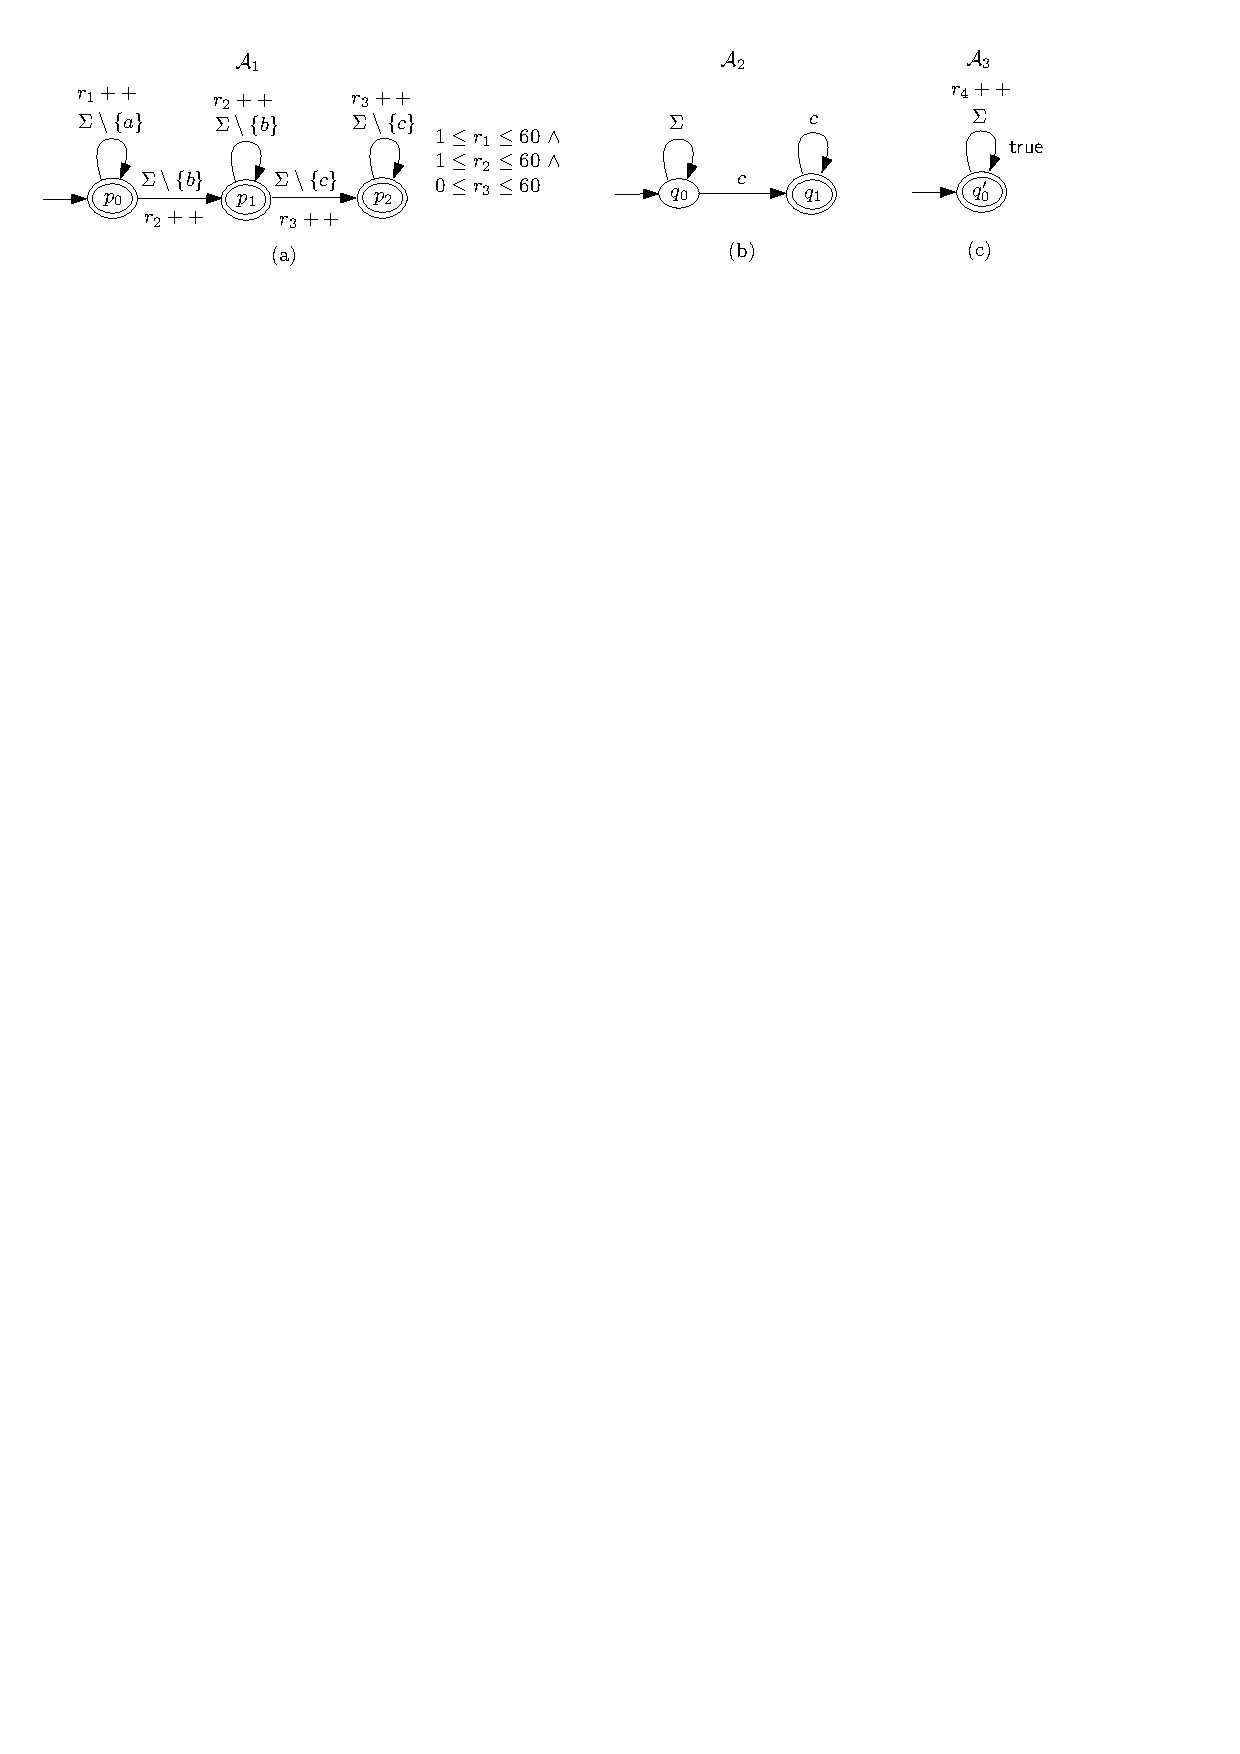
\includegraphics[width = 0.95\textwidth]{sections/overview-cefa.pdf}
  \caption{CEFA for $(\Sigma \setminus a)^{\{1, 60\}} (\Sigma \setminus b)^{\{1, 60\}} (\Sigma \setminus c)^{\{0, 60\}}$, $\Sigma^* c^+$, and $|x|$}
  \label{fig:overview}
\end{figure}

Next, 
%we remove the $\varepsilon$-transitions of $\aut_1$, resulting into $\aut'_1$, 
we construct $\aut_1 \cap \aut_2 \cap \aut_3$, that is, the intersection (aka product) of $\aut_1$, $\aut_2$, and $\aut_3$, as illustrated in Figure~\ref{fig:overview:product}(a), where the states from which no final states are reachable are removed. 
%Furthermore, we add one special register, say $r_0$, to record the length of strings. Note that $r_0$ is incremented in all transitions. 
%In $\aut_1 \cap \aut_2 \cap \aut_3$, the accepting condition $1 \le r_1 \le 60 \wedge 1 \le r_2 \le 60 \wedge 0 \le r_3 \le 60 \wedge r_0 > 120$ is attached to both $(p_0,q_1)$ and $(p_1,q_1)$, where $r_0 > 120$ is added as a conjunct to express $|x| > 120$.  
For technical convenience, we also think of the updates on the values of registers in transitions as vectors $(v_1, v_2, v_3, v_4)$, where $v_i \in \Int$ is the update on the register $r_{i}$ for each $i \in [4]$. For instance, the transitions corresponding to the self-loop around $(p_0, q_0, q'_0)$ are thought as $((p_0, q_0, q'_0), a', (p_0, q_0, q'_0), (1,0,0,1))$ with $a' \in \Sigma \setminus \{a\}$, since $r_1$ and $r_4$ are incremented in these transitions. With the updates thought of as vectors, the resulting CEFA is illustrated in Figure~\ref{fig:overview:product}(b).
%the transitions corresponding to the self-loop is $(q, a', q', (1,1,0,0))$ with $a' \in \Sigma \setminus \{a\}$.  

\begin{figure}[ht]
  \centering
  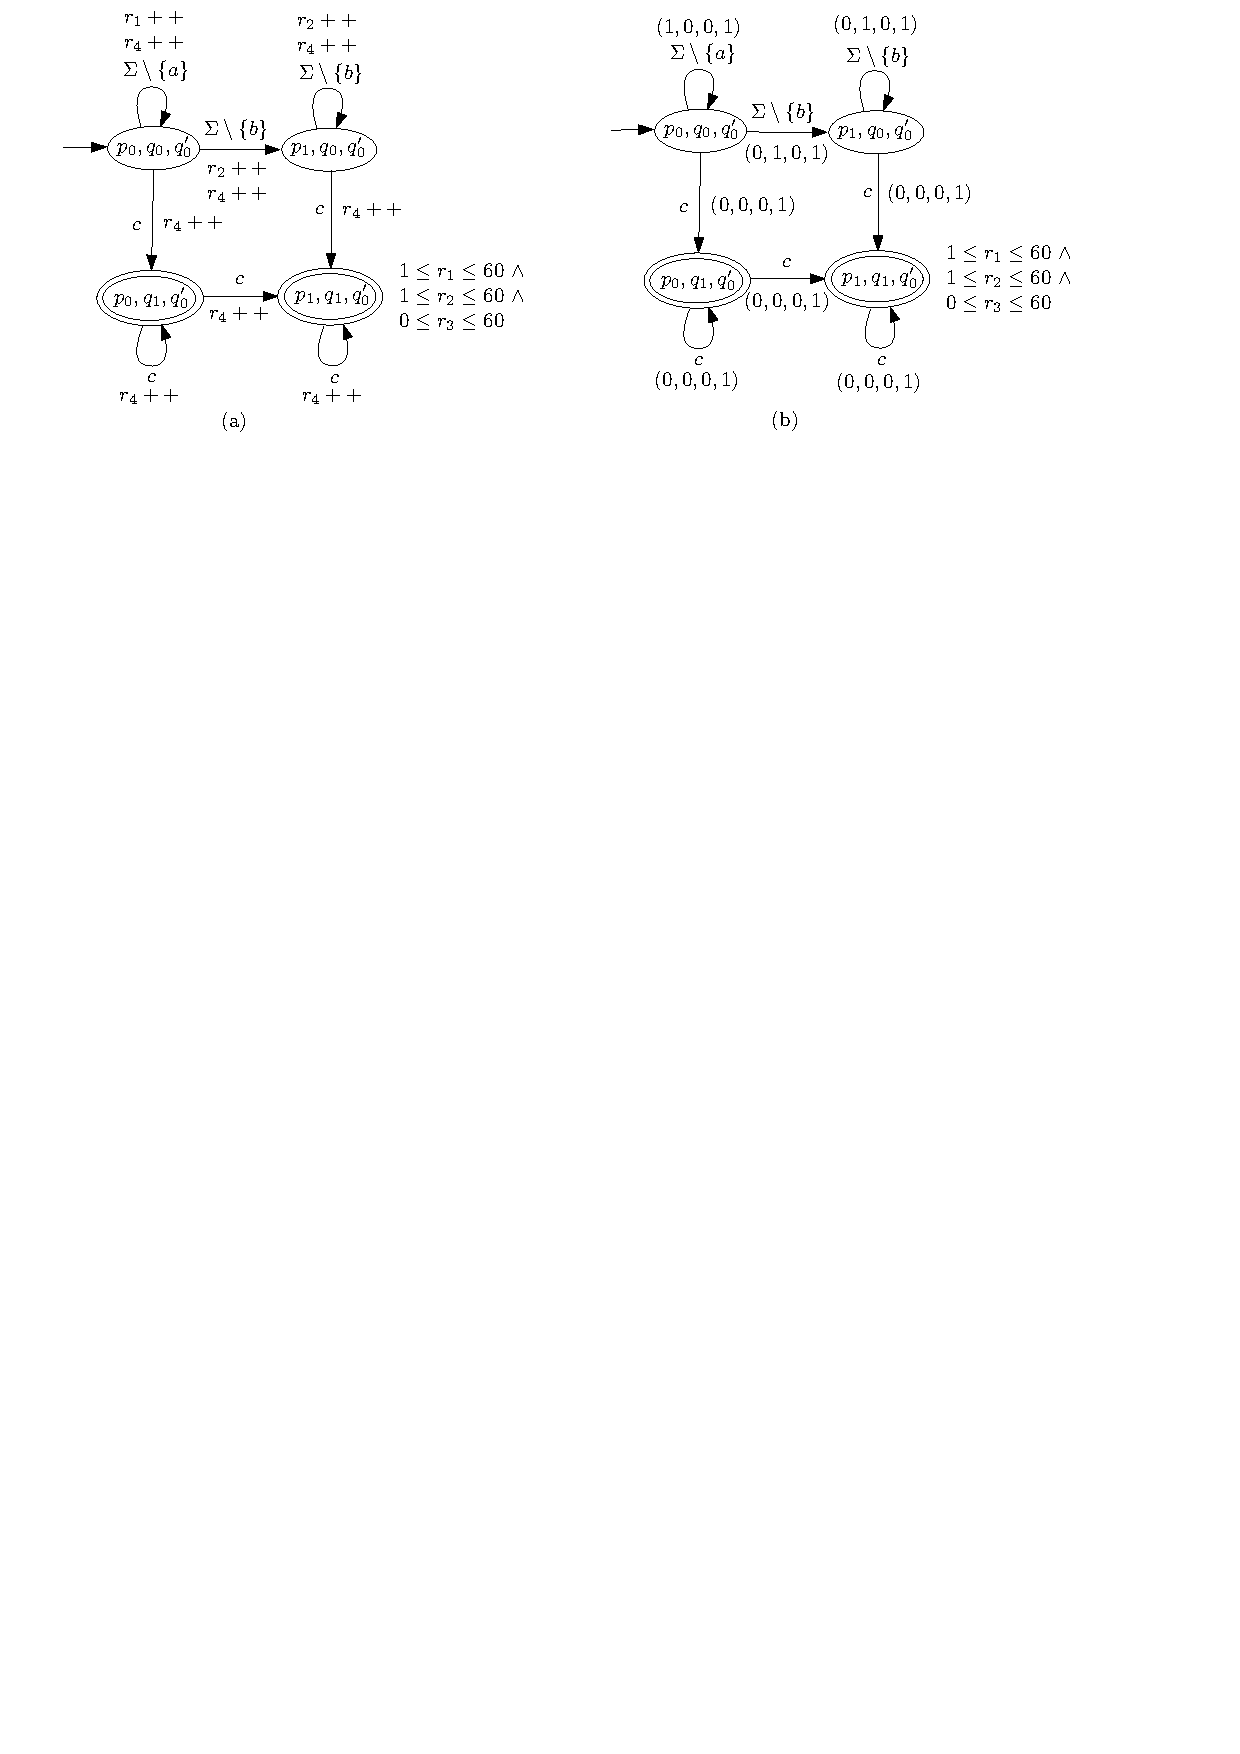
\includegraphics[width = 0.95\textwidth]{sections/overview-cefa-product.pdf}
  \caption{$\aut_1 \cap \aut_2 \cap \aut_3$: Intersection of $\aut_1$, $\aut_2$, and $\aut_3$}
  \label{fig:overview:product}
\end{figure}

%For instance, in the transition from $(p_0, q_1)$ to $(p_1, q_1)$, $r_0$ is incremented, and the values of the other registers is unchanged. Therefore, the vector for this transition is $(1, 0, 0, 0)$. 
The satisfiability of the original string constraint is reduced to the nonemptiness of the CEFA $\aut_1 \cap \aut_2 \cap \aut_3$ with respect to the LIA formula $\varphi \equiv r_4 > 120$, that is, whether there exist $w \in \Sigma^*$ and $(v_1, v_2, v_3, v_4) \in \Int^4$ such that $w$ is accepted by $\aut_1 \cap \aut_2 \cap \aut_3$, producing a cost $(v_1, v_2, v_3, v_4)$ that satisfies $1 \le v_1 \le 60\wedge 1 \le v_2 \le 60 \wedge 0 \le v_3 \le 60$ and $v_4 > 120$. 
It is not hard to observe that the nonemptiness of $\aut_1 \cap \aut_2 \cap \aut_3$ w.r.t. $\varphi \equiv r_4 > 120$ is independent of the characters of $\aut_1 \cap \aut_2 \cap \aut_3$.  Therefore, the characters in $\aut_1 \cap \aut_2 \cap \aut_3$ can be ignored, resulting into an NFA $\cB$ over the alphabet $\costset$ (see Figure~\ref{fig:overview:product:reduced}(a)), where $\costset$ is the set of vectors from $\Int^4$ occurring in the transitions of $\aut_1 \cap \aut_2 \cap \aut_3$. Then the nonemptiness of $\aut_1 \cap \aut_2 \cap \aut_3$ w.r.t. $\varphi \equiv r_4 > 120$ is reduced to the problem of deciding whether there exists $w' \in \costset^*$ such that it is accepted by $\cB$ and its Parikh image (i.e. numbers of occurrences of characters), say $\eta_{w'}: \costset \rightarrow \Nat$, satisfies that $1 \le v'_1 \le 60\wedge 1 \le v'_2 \le 60 \wedge 0 \le v'_3 \le 60$ and $v'_4 > 120$, where $\myvec{v'} = \sum \limits_{\myvec{v} \in \costset} \eta_{w'}(\myvec{v}) \myvec{v}$. Intuitively, $\myvec{v'}$ here is a weighted sum of vectors $\myvec{v} \in \costset$, where the weight for $\myvec{v}$ is the number of occurrences of $\myvec{v}$ in $w'$. (See Section~\ref{subsec:cefadec} for more detailed arguments.)

\begin{figure}[ht]
  \centering
  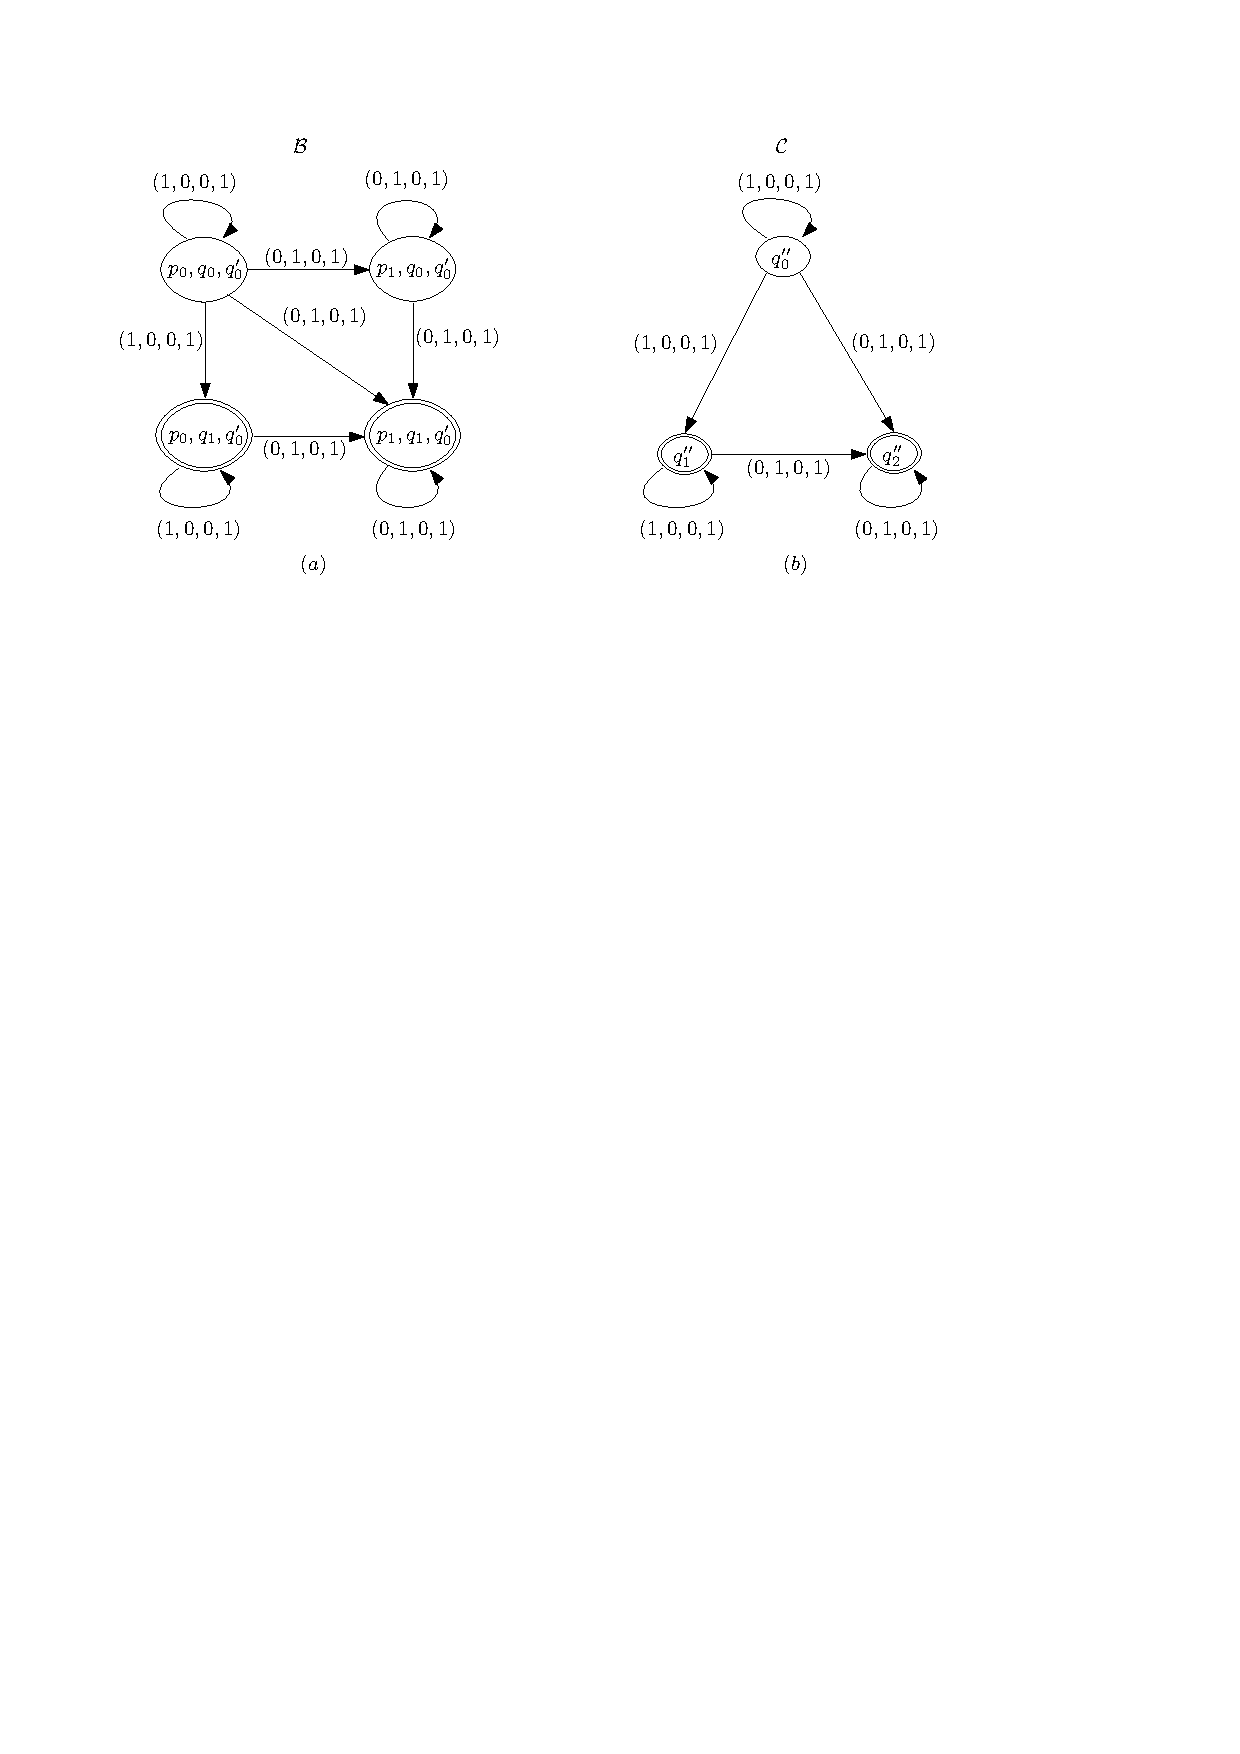
\includegraphics[width = 0.8\textwidth]{sections/overview-cefa-reduced.pdf}
  \caption{Reduced automaton $\cB$ and $\cC$}
  \label{fig:overview:product:reduced}
\end{figure}

%Let $\tau_1, \cdots, \tau_m$ be an enumeration of the transitions of $\aut_1 \cap \aut_2 \cap \aut_3$ and $\myvec{v_1}, \cdots, \myvec{v_m}$ be the vectors of updates on the registers in these transitions. 

%
Let $\costset = \{\myvec{v_1}, \cdots, \myvec{v_m}\}$. 
From the results in \cite{SSMH04,VSS05}, an existential LIA formula $\psi_\cB(\anivar_1, \cdots, \anivar_m)$ can be computed to define the Parikh image of strings that are accepted by $\cB$, where $\anivar_1, \cdots, \anivar_m$ are the integer variables to denote the number of occurrences of $\myvec{v_1}, \cdots, \myvec{v_m}$.
Therefore, the satisfiability of the string constraint in~(\ref{eqn-running}) is reduced to the satisfiability of the following existential LIA formula
\begin{equation}\label{eqn-LIA}
\begin{array}{l}
\psi_\cB(\anivar_1, \cdots, \anivar_m) \wedge \bigwedge \limits_{1 \le j \le 4} r_j = \sum \limits_{1\le k \le m}  \anivar_k v_{k, j}\ \wedge \\
1 \le r_1 \le 60 \wedge 1 \le r_2 \le 60 \wedge 0 \le r_3 \le 60 \wedge r_4 > 120.
\end{array}
\end{equation}
%where for each $k \in [m]$, $v_k = (v_{k,1}, v_{k,2}, v_{k, 3}, v_{k, 4})$ is the vector of updates on the registers $r_0, r_1, r_2, r_3$ in the transition $\tau_k$, and $\alpha(r_0, r_1, r_2, r_3)$ is the accepting condition in $\aut_1 \times \aut_2$. 
Since the satisfiability of LIA formulas can be solved by the off-the-shelf SMT solvers for LIA, the satisfiability of the string constraint in~(\ref{eqn-running}) can thus be solved.

Nevertheless, it turns out that the algorithm illustrated above is insufficient to solve the string constraints with regex-counting and string-length efficiently, since the sizes of NFA obtained from CEFA can still be big, resulting  in  the LIA formulas of big sizes, while the satisfiability of existential LIA formulas is NP-complete (see e.g. \cite{Haase18}). 
To tackle this issue, we propose techniques to reduce the sizes of NFA over the alphabet $\costset$.

%the performance could be improved if the size of the formula in~(\ref{eqn-LIA}) can be reduced. Since the size of the formula in~(\ref{eqn-LIA}) depends on the size of $\aut_1 \times \aut_2$, that is, the number of states, transitions, and registers in $\aut_1 \times \aut_2$, we propose the techniques to reduce the size of the CEFA $\aut_1 \times \aut_2$.

%Our main idea to reduce the size of the CEFA $\aut_1 \times \aut_2$ is to \emph{ignore the characters in transitions}, since the updates of the values of registers in transitions are independent of the characters therein and the satisfiability of the formula in~(\ref{eqn-LIA}) only concerns about the values of registers. After the characters in transitions are ignored, each transition in $\aut_1 \times \aut_2$ is of the form $(q, \myvec{v}, q')$, where $\myvec{v}$ is the vector denoting the updates on the values of registers. Let $\cB$ denote the resulting automaton. We then think \denghang{of} $\cB$ as an NFA, where the vectors $\myvec{v}$ are taken as the characters. 

We determinize $\cB$, apply the minimization algorithm to the resulting deterministic finite automaton (DFA), and obtain a DFA $\cC$, as illustrated in Figure~\ref{fig:overview:product:reduced}(b). 
Note that $\cC$ contains only three states $q''_0, q''_1, q''_2$ and six transitions, while $\cB$ contains four states and eight transitions. 
Although the determinization and minimization may not reduce the sizes of NFA in the worst case, the experimental results in Section~\ref{sec:implementation} show us that they do reduce the sizes of NFA constructed from the regular expressions in practice. 
%thus containing much less number of transitions than $\aut_1 \times \aut_2$\footnote{This is the case even if we consider subsets of characters, e.g. $\{a\}, \{b\}, \{c\}, \Sigma \setminus \{a, b, c\}$, in the transitions of $\aut_1 \times \aut_2$.}.
%Then we reinterpret $\cC$ as a CEFA with the acceptance condition $\alpha(r_0, r_1, r_2, r_3)$. 
%Finally, we compute an LIA formula $\psi'(i_1, \cdots, i_6)$ from $\cC$ and reduce the satisfiability of the string constraint in~(\ref{eqn-running}) to the satisfiability of the following existential LIA formula
%\begin{equation}\label{eqn-LIA-reduced}
%\psi'(i_1, \cdots, i_6) \wedge \bigwedge \limits_{0 \le j \le 3} r_j = \sum \limits_{k \in [6]}  i_k v'_{k, j+1} \wedge \alpha(r_0, r_1, r_2, r_3),
%\end{equation}
%where $\myvec{v'_{k}}=(v'_{k,1}, v'_{k,2}, v'_{k,3}, v'_{k,4})$ is the vector of updates of registers of the transition $\tau'_k$ for $k \in [6]$.

%Furthermore, we can reduce the number of registers by merging several registers into one, if they are updated with the same value in every transition of $\aut_1 \times \aut_2$. 

At last, for the string constraints that are satisfied by a collection of strings whose lengths are small, computing LIA formulas from NFA and solving them by SMT solvers are still expensive.  
Therefore, we introduce a heuristic of searching for solutions based on \emph{under approximations}, before computing LIA formulas and solving them by SMT solvers. More precisely, we enforce a constant upper bound $B$ on the lengths of strings and search for a $B$-bounded satisfiable assignment, that is, a satisfiable assignment where the lengths of strings are bound by $B$. Initially, we set $\ell$, an integer variable to denote the lengths of strings, to $1$. If there does not exist an $\ell$-bounded satisfiable assignment, then we let $\ell:=\ell+1$ and continue the search, until finding a satisfiable assignment or reaching the bound $B$. For instance, if we remove $|x| > 120$ from the string constraint~(\ref{eqn-running}), then the resulting constraint is satisfiable. Setting the bound $B$ to $3$ is sufficient to find a solution, which is witnessed by the following accepting run of $\cC$: $q^{\prime\prime}_0 \xrightarrow{(1,0,0,1)} q^{\prime\prime}_0 \xrightarrow{(0,1,0,1)} q^{\prime\prime}_1 \xrightarrow{(0,0,0,1)} q^{\prime\prime}_2$. Note that the accepting run produces $(1,1,0,3)$, a vector of register values,  which satisfies $1 \le r_1 \le 60 \wedge 1 \le r_2 \le 60 \wedge 0 \le r_3 \le 60$. (See Section~\ref{subsec:cefadec} for more details of the heuristic.)





%%%%%%%%%%%%%%%%%original texts by Denghang%%%%%%%%%%%%%%%
%%%%%%%%%%%%%%%%%original texts by Denghang%%%%%%%%%%%%%%%
\hide{
\begin{figure}[ht]
  \centering
  \import{figures}{overview_example.tex}
  \caption{The CEFA handling the difficult string constraints}
  \label{fig:overview:orgin}
\end{figure}


Recalling the string constraint listed in Section \ref{sec:intro}, DPLL(T)- and automata- based string solvers can not solve it. For DPLL(T)-based string solvers, the unsatisfiability is hard to discover since it is highly related to the length and the counting, which independent derivation rules for regex and length can not conclude. For automata-based string solvers, the counting operators result in the big-size automaton, whose length abstraction is too complex to solve. To address these issues, we use automaton to encode the semantics of the counting operator, but in a smarter way by storing counting information to registers rather than unwinding it directly. The automaton model we used is called cost-enriched finite automaton(abbreviated as regex). It is carefully discussed in Section \ref{subsec:cefa}, so we briefly introduce it in this section. A CEFA can be seen as an extension of an NFA by appending symbolic updates of integers on each transition, linear integer arithmetic to constrain the integer values on each accepting state, and registers to store integer values. The main idea is based on the observation that the occurrences of exact transitions can trace the counting times, and the length can be seen as the sum of occurrences of all transitions in the accepting run. For example, the counting times in $(\Sigma \setminus a)^{\{5, 60\}}$ can be traced by the occurrences of transitions in sub-regex $\Sigma \setminus a$. To detail, we use one register to store counting, and symbolically add 1 when running one of the transitions in $\Sigma \setminus a$, tracing the counting times. Similarly, we use another register to store the length and symbolically add 1 to it when running any transition. The automaton model of string constraints \ref{eqn-running} is illustrated in Figure \ref{fig:overview}. Register $r_1$ stores the counting times of the sub-regex $\Sigma \setminus a$, register $r_2$ stores the counting times of the sub-regex $\Sigma \setminus b$, register $r_3$ stores the counting times of the sub-regex $\Sigma \setminus c$, and register $r_4$ stores the length of the string. The label $\Sigma \setminus a:(1,0,0,1)$ means that when running the transition, the counting times of $\Sigma \setminus a$ (i.e., the value of $r_1$) plus 1, and the length (i.e., the value of $r_4$) plus 1. The accepting state $q_3$ is accepting by the linear integer arithmetic $5\leq r_1\leq 60\wedge 5\leq r_2\leq 60\wedge 0\leq r_3\leq 60\wedge 120 < r_4$. $5\leq r_1\leq 40$ ensure the counting times of $\Sigma \setminus a$ is in the range $[5, 60]$, $5\leq r_2\leq 60$ ensure the counting times of $\Sigma \setminus b$ is in the range $[5, 60]$, $0\leq r_3\leq 60$ ensure the counting times of $\Sigma \setminus c$ is in the range $[0, 60]$, and $120 < r_4$ ensure the length of the string is greater than $120$. The satisfiability of the CEFA can then be reduced to the satisfiability of linear integer arithmetic, which other off-the-shelf SMT solvers solve. \newline
However, even when we use CEFA to encode counting in the string constraints, the linear integer arithmetic reduced from the CEFA still needs to be simplified to solve. The reason is that the linear integer arithmetic is solved in exponential time of the number of variables, which is linear to the sum of transitions number and states number in the CEFA. To address this issue, we use symbolic-aware simplification to reduce the number of transitions and states in the CEFA. Simply illustrating our idea, consider a simple NFA rather than a CEFA. We assume the NFA consisted of three states $q_1, q_2, q_3$, where $q_1$ is the initial state, $q_2$ and $q_3$ are the accepting states. Assume we have three transitions from $q_1$ to $q_2$ with different characters, and three transitions from $q_1$ to $q_3$. Actually, we only need to attempt some of the six transitions to get the reachable result. We run any of the transitions, and the reachability is known. So this NFA can be simplified to two states $q_1', q_2'$ where $q_1'$ is the initial state, $q_2'$ is the accepting state, and one transition from $q_1'$ to $q_2'$ with abbreviated character. The size of NFA is sharply reduced. The simplification can be done by treating the character on each transition as the same character, then applying the minimization algorithm to the NFA. CEFA can be simplified similarly, except we need to consider the counting information, i.e., symbolic updates, on each transition. For example, $a:(1)$ and $b:(1)$ are treated as the same label but $a:(1)$ and $b:(0)$ are not. Then we can apply the minimization algorithm as NFA. Recalling the CEFA (Fig. \ref{fig:overview:orgin}) handling the string constraints \ref{eqn-running}, its transitions number between $q_1$ and $q_2$ are decided by the size of alphabet $\Sigma$. We apply symbolic-aware simplification on it, then a much smaller CEFA (Fig. \ref{fig:overview:simplified}) is obtained, whose alphabet is unary so that the number of the transition between $q_1$ and $q_2$ decreases to $1$. The state number does not decrease because these three states are not mutually equivalent. 

Sometimes the string constraints are satisfiable, and the strings in the solution have a short length. Such a solution may be quickly explored by derivation rules in DPLL(T)-based string solvers but slowly explored by our approach. To improve efficiency on satisfiable string constraints, we propose a light-way heuristic that tries to find a solution in the under-approximation of the string constraints. The main idea is to explore paths within an exact length and manually compute the registers' values, rather than reduce CEFA to heavy linear integer arithmetic. For example, consider the string constraints $x \in (\Sigma \setminus a)^{\{5, 60\}} (\Sigma \setminus b)^{\{5, 60\}} (\Sigma \setminus c)^{\{0, 60\}} \wedge x \in \Sigma^* c$, we can explore paths within length 10 and get a satisfiable solution $x = cccccccccc$. 
\begin{figure}[ht]
  \centering
  \import{figures}{overview_example.tex}
  \caption{The CEFA handling the difficult string constraints}
  \label{fig:overview:orgin}
\end{figure}
\begin{figure}[ht]
  \centering
  \import{figures}{overview_example_simplified.tex}
  \caption{The simplified CEFA handling the difficult string constraints}
  \label{fig:overview:simplified}
\end{figure}
}
%%%%%%%%%%%%%%%%%original texts by Denghang%%%%%%%%%%%%%%%
%%%%%%%%%%%%%%%%%original texts by Denghang%%%%%%%%%%%%%%%

% The main idea is to use CEFAs (see Subsection \ref{subsec:cefa}) to simulate the semantics of length operations and regular memberships with bounded repetitions. As mentioned, the ESL formula contains regular literals and linear literals. The regular literal $x\in \regex$ directly results in one CEFA recognizing it (see Subsection \ref{subsec:regex2cefa}). The linear literals $\alpha_1 \leq \alpha_2$ with no length operation remain unchanged. For each linear literal $\alpha_1 \leq \alpha_2$ with length operation $|x|$, we generate a fresh variable $i$ to replace all occurrences of $|x|$ and propagate new formula $i=|x|$. Then we generate the pre-image $\aut_{i}$ whose accepting words are strings with length $i$ (see Example \ref{eg:pre_len}). After the process above, the satisfiability problem of string constraints becomes an $SAT_{CL}$ problem, which has a decision procedure to check (see Subsection \ref{subsec:emptiness}). Example \ref{example:overview} illustrate it. \newline
% \begin{example} \label{example:overview}
%   \begin{align*}
%     \varphi\equiv x\in (ab)\{1,100\}\wedge y\in ab\wedge |x| > |y|
%   \end{align*}
%   ESL conjunction $\varphi$ is made up of regular literals $x\in (ab)\{1,100\}$ and $y\in ab$, linear literals $|x| > |y|$. The linear literal is translated to $i = |x|\wedge j = |y| \wedge i > j$. Our algorithm solves the formula in four steps. First, we construct CEFAs for regular memberships $x\in (ab)\{1,100\}$ and $y\in ab$ (Fig.\ref{subfig:aut_ab1-100} and Fig.\ref{subfig:aut_ab}). Second, we compute the pre-images of length operations $i=|x|$ and $j=|y|$ (Fig.\ref{subfig:preimage_x} and Fig.\ref{subfig:preimage_y}). Then we intersect pre-images to automata corresponding to the regular memberships for each string variable (Fig.\ref{subfig:aut_x} and Fig.\ref{subfig:aut_y}). We translate the satisfiability problem of $\varphi$ to the emptiness checking problem of automata (Fig.\ref{subfig:preimage_x} and Fig.\ref{subfig:preimage_y}) under linear arithmetic constants $i > y$, which could be solved by the decision procedure illustrated in section \ref{sec:algorithm}.

  % \begin{figure}[h]
  %   \begin{subfigure}[b]{0.49\textwidth}
  %     \centering
  %     \begin{tikzpicture}[
  %       shorten >=1pt,node distance=2cm,on grid,>={Stealth[round]},
  %       initial text=, every state/.style={minimum size = 0.001cm},
  %       accepting text=$1\leq r_1\leq 100$, accepting/.style=accepting by arrow,
  %       accepting where=above
  %       ]

  %       \node[state,initial]            (q_0)                      {};
  %       \node[state]                    (q_1) [right=of q_0]       {};
  %       \node[state,accepting]          (q_2) [right=of q_1]       {};

  %       \path[->] (q_0) edge              node      [above]           {$a$/(1)} (q_1)
  %       (q_1) edge              node      [above]           {$b$/(0)} (q_2)
  %       (q_2) edge [bend left]  node      [below]           {$a$/(1)} (q_1);
  %     \end{tikzpicture}
  %     \caption{The CEFA recognizing $(ab)\{1,100\}$}
  %     \label{subfig:aut_ab1-100}
  %   \end{subfigure}
  %   \begin{subfigure}[b]{0.49\textwidth}
  %     \centering
  %     \begin{tikzpicture}[
  %       shorten >=1pt,node distance=2cm,on grid,>={Stealth[round]},
  %       initial text=, every state/.style={minimum size = 0.001cm},
  %       accepting text=$\top$, accepting/.style=accepting by arrow,
  %       accepting where=above
  %       ]

  %       \node[state,initial]            (q_0)                      {};
  %       \node[state]                    (q_1) [right=of q_0]       {};
  %       \node[state, accepting]         (q_2) [right=of q_1]       {};

  %       \path[->] (q_0) edge              node      [above]           {$a$/()} (q_1)
  %       (q_1) edge              node      [above]           {$b$/()} (q_2);
  %     \end{tikzpicture}
  %     \caption{The CEFA recognizing $ab$}
  %     \label{subfig:aut_ab}
  %   \end{subfigure}
  %   \begin{subfigure}[b]{0.49\textwidth}
  %     \centering
  %     \begin{tikzpicture}[
  %       shorten >=1pt,node distance=2cm,on grid,>={Stealth[round]},
  %       initial text=, every state/.style={minimum size = 0.001cm},
  %       accepting text=${r_2 = i}$, accepting/.style=accepting by arrow,
  %       ]

  %       \node[state,initial,accepting]            (q_0)       {};

  %       \path[->] (q_0) edge [loop below] node{$\Sigma$/(1)} ();
  %     \end{tikzpicture}
  %     \caption{The pre-image of $i = |x|$}
  %     \label{subfig:preimage_x}
  %   \end{subfigure}
  %   \begin{subfigure}[b]{0.49\textwidth}
  %     \centering
  %     \begin{tikzpicture}[
  %       shorten >=1pt,node distance=2cm,on grid,>={Stealth[round]},
  %       initial text=, every state/.style={minimum size = 0.001cm},
  %       accepting text=${r_3 = j}$, accepting/.style=accepting by arrow,
  %       ]

  %       \node[state,initial,accepting]            (q_0)       {};

  %       \path[->] (q_0) edge [loop below] node{$\Sigma$/(1)} (1);
  %     \end{tikzpicture}
  %     \caption{The pre-image of $j = |y|$}
  %     \label{subfig:preimage_y}
  %   \end{subfigure}
  %   \begin{subfigure}[b]{0.49\textwidth}
  %     \centering
  %     \begin{tikzpicture}[
  %       shorten >=1pt,node distance=2cm,on grid,>={Stealth[round]},
  %       initial text=, every state/.style={minimum size = 0.001cm},
  %       accepting text=${r_2 = i\wedge 1\leq r_1 \leq 100}$, accepting/.style=accepting by arrow,
  %       accepting where=above
  %       ]

  %       \node[state,initial]            (q_0)                      {};
  %       \node[state]                    (q_1) [right=of q_0]       {};
  %       \node[state,accepting]          (q_2) [right=of q_1]       {};

  %       \path[->] (q_0) edge node [above]  {$a$/(1,1)} (q_1)
  %       (q_1) edge           node [above]  {$b$/(0,1)} (q_2)
  %       (q_2) edge [bend left]  node      [below]           {$a$/(1,1)} (q_1);
  %     \end{tikzpicture}
  %     \caption{The final automaton of $x$}
  %     \label{subfig:aut_x}
  %   \end{subfigure}
  %   \begin{subfigure}[b]{0.49\textwidth}
  %     \centering
  %     \begin{tikzpicture}[
  %       shorten >=1pt,node distance=2cm,on grid,>={Stealth[round]},
  %       initial text=, every state/.style={minimum size = 0.001cm},
  %       accepting text=${r_3=j}$, accepting/.style=accepting by arrow,
  %       accepting where=above
  %       ]

  %       \node[state,initial]            (q_0)                      {};
  %       \node[state]                    (q_1) [right=of q_0]       {};
  %       \node[state, accepting]         (q_2) [right=of q_1]       {};

  %       \path[->] (q_0) edge    node      [above]           {$a$/(1)} (q_1)
  %       (q_1) edge              node      [above]           {$b$/(1)} (q_2);
  %     \end{tikzpicture}
  %     \caption{The final automaton of $y$}
  %     \label{subfig:aut_y}
  %   \end{subfigure}
  %   \caption{All automata used in the example \ref{example:overview}}
  % \end{figure}


% \end{example}

% \pagebreak

The wrong encoding of the backslash causes the soundness errors of z3str3re. Two backslashes are seen as two characters in the Smtlib2.6 standard, but z3str3re encodes them as one.

%\vspace{-2mm}
\section{String constraints with regex-counting and string-length}\label{sec:recl}
%\vspace{-2mm}
%!TEX root = ../main.tex
%\documentclass{standalone}
%\begin{document}

%\subsubsection{Syntax}
In the sequel, we define string constraints with regex-counting and string-length function (abbreviated as RECL). The syntax of RECL is defined by the rules in Table~\ref{tab:syntax}. 
A RECL formula $\varphi$ is a conjunction of atomic formulas of the form $x \in \regex$, $x \not \in \regex$, or $t_1\ \op\ t_2$, where $x$ is a string variable, $\regex$ is a regular expression,  
$t_1$ and $t_2$ are integer terms, and $\op \in \{=, \neq, \le, \ge, <, >\}$. Atomic formulas of the form $x \in \regex$ or $x \not \in \regex$ are called \emph{regular membership} constraints and atomic formulas of the form $t_1\ \op\ t_2$ are called \emph{length} constraints. 
%
A regular expression $\regex$ is built from $\emptyset$, the empty string $\epsilon$, and characters $a$ by using concatenation  $\cdot$, alternation $+$, Kleene star $^*$, intersection $\cap$, complement $\bar{\mbox{ }}$, difference $\setminus$, counting $^{\{m,n\}}$ or $^{\{m,\infty\}}$. 
% 
%is a quantifier-free formula that can be a regular membership $x\in\regex$, a quantifier-free Presburger formula $\alpha_1 \leq \alpha_2$, a negation of a formula, or a disjunction of two formulas. $\alpha$ is an integer term which can be an integer constant $m$, integer variable $i$, the length of the string term $|s|$, the minus of an integer term, and the plus of two integer terms. The regular expression $\regex$ is built on empty string $\epsilon$, constant letter $a\in \Sigma$. The supported regex operations involve concatenation $\cdot$, disjunction $+$, intersection $\times$, closure $*$, complement $C$, and bounded repetition $\{m, n\}$. We use $term(\varphi)$ to denote the set of terms and $strvar(\varphi)$ to denote the string variables occurring in $\varphi$. The \emph{literals} of $\varphi$ are $x\in \regex$ and $\alpha_1 \leq \alpha_2$. $x\in \regex$ is called \emph{regular literals} and $\alpha_1 \leq \alpha_2$ is called \emph{linear literals}.
\begin{table}[h]
  \centering
  \begin{tabular}{l r}
    $\varphi$ ::= $x\in \regex \mid x \not \in \regex \mid t_1\  \op\ t_2 \mid  \varphi \wedge \varphi $                                             & formulas            \\
    $\regex$ ::= $\emptyset \mid \epsilon \mid a \mid \regex\cdot \regex \mid \regex+\regex \mid \regex^* \mid \regex \cap \regex \mid \overline{\regex} \mid \regex \setminus \regex \mid \regex^{\{m,n\}} \mid \regex^{\{m,\infty\}}$ & regular expressions \\
    $t$ ::= $n \mid i \mid  |x| \mid t - t \mid t + t$                                                                       & integer terms
  \end{tabular}
  \caption{Syntax of RECL }\label{tab:syntax}
\end{table}
% Semantic 

\zhilin{stopped here}

%\subsubsection{Semantic}
We assume that $S$ is the set of string variables over $\Sigma^*$, and $I$ is the set of integer variables. $\eta: S\times\Sigma\rightarrow\Sigma^*$ is the interpretation on string where $\eta(c)=c$ for every letter $c\in \Sigma$. $\pi: I\rightarrow\mathbb{Z}$ is the interpretation of Presburger arithmetic. Then the semantics is given by a satisfaction relation: $\eta, \pi\models \varphi$ defined in Table \ref{tab:semantics}. We say a formula $\varphi$ is \emph{satisfiable} if a solution $(\eta, \pi)$ exists such as $\eta, \pi\models \varphi$. A formula $\varphi$ is \emph{unsatisfiable} if no solution exists.
\begin{table}[h]
  \centering
  \begin{tabular}{lcl}
    $\eta,\pi \models \varphi_1\vee \varphi_2$ & $\mathsf{iff}$ & $\eta,\pi \models \varphi_1 \text{ or } \eta,\pi \models \varphi_2$ \\
    $\eta,\pi \models \neg\varphi $            & $\mathsf{iff}$ & $\eta,\pi \not\models \varphi$                                      \\
    $\eta, \pi \models x\in \regex$            & $\mathsf{iff}$ & $\exists w \in \lan(\regex),\eta,\pi \models x = w$                 \\
    $\eta, \pi \models \alpha_1 \leq \alpha_2$ & $\mathsf{iff}$ & $\pi(\alpha_1) \leq \pi(\alpha_2) $                                 \\
  \end{tabular}
  \caption{Semantics}
  \label{tab:semantics}
\end{table}
In addition to the classic regex operators (union, concatenation, closure), we syntactically support intersection, complement, and repetition. As we all know, the classic regular language is closed under intersection and complement \cite{aut_hopcraft}. Furthermore, the operation \emph{repetition} $\regex\{m,n\}$ means repeating regex $\regex$ at least $m$ times and at most $n$ times. It can be syntactically rewritten by concatenation and union:
$\regex\{m,n\} \equiv \regex^m\mid\cdots\mid\regex^n$ where $\regex^k$ defines concatenate $\regex$ $k$ times ($m\leq k\leq n$). So the regular language $\lan(\regex)$ defined in Table \ref{tab:syntax} is semantically equal to the classic regular language.

%\end{document}

%\vspace{-2mm}
\section{Cost-enriched finite automata} \label{sec:automaton}
%\vspace{-2mm}
%!TEX root = ../main.tex
%\documentclass{standalone}
%\begin{document}

In this section, we define the model of cost-enriched finite state automata (CEFA), which was introduced in \cite{atva2020} and will be used to solve the satisfiability problem of RECL later on. 
%
Intuitively, CEFA add write-only cost registers to finite state automata. Here by ``write-only'', we mean that the cost registers can only be written/updated, but cannot be read, that is, cannot be used to guard the transitions. 

%
%In~\cite{atva2020}, the cost function is defined as a function $\eta: \Sigma \rightarrow \mathbb{N}$. In this paper, we define the cost function as an integer vector whose elements are the incremental value of registers. Furthermore, we add a new linear integer arithmetic constraint $\theta$ to each final state of the CEFA, which restricts the value of registers. Two types of definitions have the same expressive ability on the $SAT_{CL}$ problem.
\begin{definition}[Cost-Enriched Finite Automaton]
  A cost-enriched finite automaton $\aut$ is a tuple $(R, Q, \Sigma, \delta, q_0, F, \theta)$ where
  \begin{itemize}
  \item $R = \{r_1, \cdots, r_k\}$ is a finite set of registers, 
    \item $Q, \Sigma, q_0, F$ are as in the definition of NFA,
%    \item $R = (r_1\cdots r_n)$ is a vector of mutually distinct cost registers,
    \item $\delta \subseteq Q \times \Sigma_\varepsilon \times Q \times \Int^R$ is a transition relation, where $\Int^R$ denotes the updates on the values of registers, 
%  set whose elements are tuples $(q, c, q', \myvec{v})$ where $q, q'$ are states of $Q$, $c$ is a letter in alphabet $\Sigma\cup\{\epsilon\}$ and $\myvec{v}$ is the cost update function for registers, which is an integer vector whose $i$-th element is the incremental value of register $r_i$.  $(q, a, q', \myvec{v})$ is written as $q\xrightarrow[\myvec{v}]{a} q'$ for readability.
    \item $\alpha: F \rightarrow \Phi(R)$ attaches to each finite state an accepting condition that is specified by an LIA formula.
%    a linear integer arithmetic constraint function on final states. $\theta$ is called \emph{accepting condition}.
  \end{itemize}
\end{definition}
The definition of CEFA above is slightly different from the definition in~\cite{atva2020} in the sense that accepting conditions on register values
are attached to final states. 

For readability, we assume a linear order on $R$ and write $R$ as a vector $\myvec{r} = (r_1, \cdots, r_k)$. Moreover, we write an element of $\Int^R$ as a vector $(v_1, \cdots, v_k)$, where for each $i \in [k]$, $v_i$ is the update on the value of $r_i$. We also write a transition $(q, a, q', \vec{v}) \in \delta$ as $q \xrightarrow[\vec{v}]{a} q'$.



The semantics of CEFA is define as follows. Let $\aut = (R, Q, \Sigma, \delta, q_0, F, \alpha)$ be a CEFA. 
A \emph{configuration} of $\aut$ is a pair $(q, \vec{v})$ where $q \in Q$ and $\vec{v}$ is a vector denoting the values of registers.  
The \emph{initial configuration} of $\aut$ is $(q_0, \vec{0})$, where the value of each register is zero. 
A \emph{run} of $\aut$ on a string $w = a_1 \cdots a_n$ is a sequence $q_0 \xrightarrow[\myvec{v_1}]{b_1} q_1 \cdots q_{m-1}\xrightarrow[\myvec{v_m}]{b_m} q_m$ such that $w = b_1 \cdots b_m$ (some of $b_i$'s may be $\varepsilon$) and $q_{i-1} \xrightarrow[\myvec{v_i}]{b_i} q_i$ for each $i \in [m]$. A run $q_0 \xrightarrow[\myvec{v_1}]{b_1} q_1 \cdots q_{m-1}\xrightarrow[\myvec{v_m}]{b_m} q_m$ is \emph{accepting} if $q_m \in F$ and $\alpha(q_m)[\myvec{\myvec{v'}/\myvec{r}]$ is true, where $\myvec{v'} = \sum \limits_{j \in [m]} \myvec{v_j}}$. Note here we assume that the initial values of all registers are zero and $\sum \limits_{j \in [m]} \myvec{v_j}$ is the vector of register values after all the transitions in the run are executed. A string $w$ is \emph{accepted} by $\aut$ if there is an accepting run of $\aut$ on $w$. The language defined by $\aut$, denoted by $\Lang(\aut)$, is the set of strings that are accepted by $\aut$. 

%The value of each register $r_i$ in $R$ is written as $\mathcal{V}(r_i)$ and is initiated to 0 at the initial state. A \emph{run} of $\aut$ on string $a_1\cdots a_m$ is a transition sequence $q_I\xrightarrow[\myvec{v_1}]{a_1}q_1\cdots q_{m-1}\xrightarrow[\myvec{v_m}]{a_m}q_m$  and $\mathcal{V}(r_i) = \displaystyle\sum_{j=1}^m \myvec{v_j}[i], i\in [1,n]$ is the value of $r_i$ after the run. $\theta[R/\mathcal{V}(R)](q_m)$ is obtained from $\theta(q_m)$ by replacing each register $r_i$ to its value $\mathcal{V}(r_i)$. The run is \emph{accepting} if $q_m\in F$ and $\theta[R/\mathcal{V}(R)](q_m)$ is satisfiable. $\top$ is the valid formula that is always satisfiable. A string $w$ is accepted by $\aut$ if it has an accepting run of $\aut$. The language of $\aut$ is the set of strings accepted by $\aut$, denoted by $\lan(\aut)$.

\zhilin{this example should be modified to match the running example}
\begin{example} \label{eg:1}
  Fig.\ref{fig:repetition} illustrates the CEFA recognizing $(ab)\{1,100\}$. The register vector is $(r_1)$, and the linear arithmetic constraint on $q_2$ is $1\leq r_1\leq 100$. Intuitively, the transition $q_0 \xrightarrow[(1)]{a} q_1$ accept the char $a$ and increase 1 on the value of $r_1$. The transition $q_1 \xrightarrow[(0)]{b} q_2$ accepts the char $b$ and does not change the value. The transition $q_2 \xrightarrow[(0)]{\epsilon} q_2$ is a nondeterministic choice back to initial state $q_0$. Because of the linear arithmetic constraint $1\leq r_1\leq 100$, the value of $r_1$ in the accepting run must be $[1,100]$. $\mathcal{V}(r_1)$ equal to the occurrence number of the transition $q_0 \xrightarrow[(1)]{a} q_1$, so that the accepted string is $ab\cdots ab$ in which $a$ appears at least once and at most 100 times. That is, the language of the automaton is $(ab)\{1,100\}$.
  \begin{figure}[h]
    \centering
    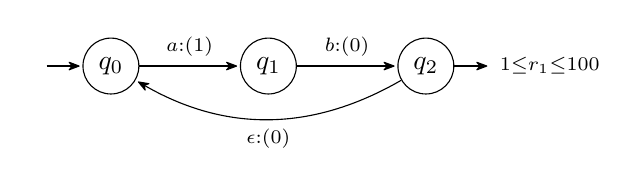
\begin{tikzpicture}[
      shorten >=1pt,node distance=2cm,on grid,>={Stealth[round]},
      initial text=, every state/.style={minimum size = 0.001cm,
          accepting text=$\scriptstyle 1\leq r_1\leq 100$, accepting/.style=accepting by arrow}
      ]
      \node[state,initial]            (q_0)                      {$q_0$};
      \node[state]                    (q_1) [right=of q_0]       {$q_1$};
      \node[state,accepting]          (q_2) [right=of q_1]       {$q_2$};

      \path[->] (q_0) edge              node      [above]           {$\scriptstyle a:(1)$} (q_1)
      (q_1) edge              node      [above]           {$\scriptstyle b:(0)$} (q_2)
      (q_2) edge [bend left]  node      [below]           {$\scriptstyle\epsilon: (0)$} (q_0);
    \end{tikzpicture}
    \caption{An automaton recognizing the language of $(ab)\{1,100\}$}
    \label{fig:repetition}
  \end{figure}
\end{example}


% Parikh's theorem \cite{parikh_theorem}\cite{parikh_anthony}\cite{parikh_compute} states that the Parikh image of a context-free language is semilinear so that it can be written as Presburger formula. Following the version for context-free grammar \cite{parikh_compute} and the version for regular expression \cite{parikh_for_nfa}, we define the Parikh image of language of an CEFA $\aut = (Q, \Sigma, \delta, q_I, F, R, \theta)$  as follows:
% \begin{table}[h]
%   \begin{tabular}{l l r}
%     $\psi(\aut)\equiv$& $\bigwedge\limits_{q\in Q}(\text{$f_q$ if $q\in F$ otherwise 0}) + \sum\limits_{(q,a,q',\myvec{v})\in\delta} t_{q,a,q',\myvec{v}} = $ & \\
%     & \quad \ \ (1 if $q = q_I$ otherwise 0) + $\sum\limits_{(q',a,q,\myvec{v})\in\delta} t_{q',a,q, \myvec{v}} $ & \\ 
%     & $\bigwedge\limits_{(q,a,q',\myvec{v})\in\delta} t_{q,a,q',\myvec{v}}\geq 0$ & (consistent formula)\\
%     & & \\
%     & $\bigwedge\limits_{(q,a,q',\myvec{v})\in\delta} t_{q,a,q',\myvec{v}}>0\rightarrow z_{q'} > 0$ & \\
%     & $\bigwedge\limits_{q\in F} z_q > 0\rightarrow f_q = 1$ & \\ 
%     & $\bigwedge\limits_{q\in Q} z_q > 0\rightarrow \bigvee\limits_{(q,a,q',\myvec{v})\in\delta} z_q = z_{q'} + 1\wedge t_{q,a,q',\myvec{v}}\geq 0 \wedge z_{q'} > 0$& (connected formula)\\
%     & & \\
%     &$\bigwedge\limits_{r_i\in R} r_i = \sum\limits_{(q,a,q',\myvec{v})\in \delta} t_{q,a,q',\myvec{v}}*\myvec{v}[i]$ & (register value formula)\\
%     & & \\
%     &$\bigwedge\limits_{q\in F} f_q > 0 \rightarrow \theta(q)$ & (accepting condition) 
%   \end{tabular}
% \end{table}
% $z_q$ is the distance of state $q$ from $q_f\in F$ in a spanning tree. $t_{q,a,q',\myvec{v}}$ represents the using times of transition $(q,a,q',\myvec{v})$ in the accepting run. $f_q$ stands for whether an accepting state $q\in F$ is the final state of a run. The Parikh image of $\aut$ is a Presburger formula $\psi(\aut)$, which is consistent and connected. The register value formula ensures the register values are correctly updated regarding the accepting run. 
% \begin{example} \label{exapmle:parikh}
%   Suppose that we have a CEFA $\aut$ shown in Fig. \ref{subfig:aut_x}. Using $t_1, t_2, t_3$ to record the times of transitions in the accepting run of $\aut$, the Parikh image $\psi(\aut)$ is the quantifier-free Presburger formula $\psi_{cons}\wedge \psi_{conn} \wedge \psi_{val} \wedge \psi_{aut}$ where:
%   \begin{itemize}
%     \item $\psi_{cons} \equiv 1 = t_1 \wedge t_1 + t_3 = t_2 \wedge t_2 = t_3 + 1 \bigwedge\limits_{i\in[1,3]} t_i\geq 0$ is the consistent formula.
%     \item $\psi_{conn} \equiv \top $ is the connectivity formula because all transitions in $\aut$ are connected.
%     \item $\psi_{val} \equiv r_1=t_1 + t_3\wedge r_2 = t_1+t_2+t_3$ is the formula deciding the value of $r_1$ and $r_2$ after a run.
%     \item $\psi_{aut} \equiv r_2 = i\wedge 1 \leq r_1 \leq 100$ is the accepting condition of $\aut$.
%   \end{itemize}
%   $\psi(\aut)$ can be simplified to $t_3\geq 0 \wedge t_1=1\wedge r_1 = t_3 + 1\wedge r_2 = 2*t_3+2\wedge r_2=i\wedge 1\leq r_1\leq 100$. A possible solution is $t_1 =1, t_3 = 0, r_1=1, r_2=2$ and the corresponding accepted string $ab$. It is obvious that $r_1$ is the repeat times of $ab$ and $r_2$ is the length of $ab$.
% \end{example}
%\end{document}

%\vspace{-2mm}
\section{Solving RECL constraints} \label{sec:algorithm}
%\vspace{-2mm}
%!TEX root = ../main.tex
%\documentclass{standalone}
%\begin{document}

This section aims to show how to solve RECL constraints by utilizing CEFA. 
At first, we reduce the satisfiability of RECL constraints to a decision problem defined in the following section. Then we propose an algorithm to solve the decision problem. 

% \vspace{-2mm}
\begin{definition}[Nonemptiness of CEFA w.r.t. an LIA formula
% \footnote{The decision problem was called satisfiability of an LIA formula w.r.t. CEFA in \cite{atva2020}.}
, abbreviated as $\cefadec$]
Suppose that $x_1, \cdots, x_n$ are string variables, $\Lambda_{x_1}, \cdots, \Lambda_{x_n}$ are nonempty sets of CEFA over the alphabet $\Sigma$ with $\Lambda_{x_i} = \{\aut_{i, 1}, \cdots, \aut_{i, l_i}\}$ for every $i \in [n]$, and the sets of registers $R_{\aut_{1, 1}}, \cdots, R_{\aut_{1, l_1}}, \cdots, R_{\aut_{n, 1}}, \cdots, R_{\aut_{n, l_n}}$ are mutually disjoint, moreover, $\varphi$ is an LIA formula whose free variables are from $ \bigcup \limits_{i \in [n], j \in [l_i]} R_{\aut_{i, j}}$. Then  the CEFA in $\Lambda_{x_1}, \cdots, \Lambda_{x_n}$ are said to be nonempty w.r.t. $\varphi$ if there are assignments $\theta: \{x_1, \cdots, x_n\} \rightarrow \Sigma^*$ and vectors $\myvec{v_{i,j}}$
%$\myvec{v_{1,1}}, \cdots, \myvec{v_{1, l_1}}, \cdots, \myvec{v_{n, 1}}, \cdots, \myvec{v_{n, l_n}}$ 
such that $(\theta(x_i); \myvec{v_{i,j}}) \in \Lang(\aut_{i, j})$ and  $\varphi[(\myvec{v_{i,j}}/R_{\aut_{i,j}})]$ is true, for every $i \in [n], j \in [l_i]$.
% \in \aut_{i,1}(\eta(x_1)), \cdots, \myvec{v_{i, l_i}} \in \aut_{i,l_i}(\eta(x_i))$ for every $i \in [n]$  
%\cdots, \myvec{v_{n,1}} \in \aut_{n,1}(w_n), \cdots, \myvec{v_{n, l_n}} \in \aut_{n, l_n}(w_n)$ 
% $\varphi[(\myvec{v_{i,j}}/R_{\aut_{i,j}})_{i \in [n], j \in [l_i]}]$ is true. 
%$\varphi[\myvec{v_{1,1}}/R_{\aut_{1,1}}, \cdots, \myvec{v_{n, l_n}}/R_{\aut_{n, l_n}}]$ is true. 
\end{definition}
% \vspace{-4mm}
\begin{proposition}\label{prop-cefadec}
$\cefadec$ is PSPACE-complete. 
\end{proposition}
\begin{proof}
  The lower bound follows from the fact that the nonemptiness problem of the intersection of NFAs is PSPACE-complete \cite{pspace_int}. For the upper bound, \cite{atva2020} showed that $\cefadec$ is in PSPACE by reducing it to monotonic counter machines.
\end{proof}
Note that the decision procedure in \cite{atva2020} was only used to prove the upper bound in Proposition~\ref{prop-cefadec} and not implemented as a matter of fact. Instead, the symbolic model checker nuXmv was used to solve $\cefadec$. We do not rely on nuXmv in this work and shall propose a new algorithm for solving $\cefadec$ in Section~\ref{subsec:cefadec}. 

%As mentioned in Section \ref{sec:overview}, the main idea of our approach is to model the counting operators symbolically by registers instead of unfolding them explicitly. Additionally, we use registers to represent string lengths. After that, the satisfiability of string constraints involves regex-counting, and string-length is reduced to the satisfiability of LIA, which off-the-shelf SMT solvers can solve. We also propose techniques to reduce automata sizes and utilize under approximations to enhance performance.
\vspace{-2mm}
\subsection{From $\reclsat$ to $\cefadec$} \label{subsec:regex2cefa}
\vspace{-1mm}

Let $\varphi$ be a RECL constraint and $x_1, \cdots, x_n$ be an enumeration of the string variables occurring in $\varphi$. Moreover, let $\varphi \equiv \varphi_1 \wedge \varphi_2$ such that $\varphi_1$ is a conjunction of regular membership constraints of $\varphi$, and $\varphi_2$ is a conjunction of length constraints of $\varphi$.
We shall reduce the satisfiability of $\varphi$ to an instance of $\cefadec$. 

At first, we show how to construct a CEFA from a regular expression where counting operators may occur. 
Let us start with register-representable regular expressions defined in the sequel. 

Let us fix an alphabet $\Sigma$.

Let $e$ be a regular expression over $\Sigma$. Then an occurrence of counting operators in $e$, say $(e')^{\{m,n\}}$ (or $(e')^{\{m, \infty\}}$), is said to be \emph{register-representable} if $(e')^{\{m,n\}}$ (or $(e')^{\{m, \infty\}}$) is not in the scope of a Kleene star, another counting operator, complement, or language difference in $e$. We say that $e$ is \emph{register-representable} if all occurrences of counting operators in $e$ are register-representable. For instance, $(a^{\{2, 6\}} \concat b^*) \cap (a + b)^{\{4, \infty\}}$ is register-representable, while $(a^{\{2, 6\}} \concat b^*) \setminus (a + b)^{\{4, \infty\}}$ and $(a^{\{2, 6\}} \concat b^*)^{\{2,\infty\}}$ are not since $a^{\{2,6\}}$ is in the scope of language difference and the counter operator $\{2, \infty\}$ respectively.  

Let $e$ be a register-representable regular expression over $\Sigma$. By the following procedure, we will construct a CEFA out of $e$, denoted by $\aut_e$. 
\vspace{-1mm}
\begin{enumerate}
%
\item For each sub-expression $(e')^{\{m,n\}}$ with $m \le n$ (resp. $(e')^{\{m, \infty\}}$) of $e$, we construct a CEFA $\aut_{(e')^{\{m,n\}}}$ (resp. $\aut_{(e')^{\{m, \infty\}}}$) as follows. Let $\aut_{e'} = (Q, \Sigma, \delta, I, F)$. Same as the construction for Kleene star except for the new register and updates on transitions, $\aut_{(e')^{\{m,n\}}} = ((r'), Q', \Sigma, \delta'', I', F', \alpha')$, where $r'$ is a new register, 
%
\vspace{-3mm}
$$
\begin{array}{l c l}
\delta'' & = & \{(q, a, q', (0)) \mid (q, a, q') \in \delta\}\  \cup \\
& & \{(q_0, a, q', (1))  \mid \exists q'_0 \in I.\ (q'_0, a, q') \in \delta\}\ \cup \\
& & \{(q, a, q', (1)) \mid q \in F, \exists q'_0 \in I.\ (q'_0, a, q') \in \delta\},
\end{array}
$$ 
%
moreover, $\alpha' = m \le r' \le n$ if $I \cap F = \emptyset$, otherwise $\alpha' = r' \le n$ .  (Intuitively, if $\varepsilon$ is accepted by $\aut_{e'}$, then the value of $r'$ can be less than $m$.) Finally, $\aut_{(e')^{\{m, \infty\}}}$ is constructed by adapting $\alpha'$ in $\aut_{(e')^{\{m,n\}}}$ as follows: $\alpha' = m \le r'$ if $I \cap F = \emptyset$ and $\alpha' = \ltrue$ otherwise. 
%

\item For each sub-expression $e'$ of $e$ such that $e'$ contains occurrences of counting operators but $e'$ itself is not of the form $(e'_1)^{\{m,n\}}$ or $(e'_1)^{\{m,\infty\}}$, from the assumption that $e$ is register-representable, we know that $e'$ is of the form $e'_1 \concat e'_2$, $e'_1 + e'_2$, $e'_1 \cap e'_2$, or $(e'_1)$. For $e' = (e'_1)$, we have $\aut_{e'} = \aut_{e'_1}$. For $e' = e'_1 \concat e'_2$, $e' = e'_1 + e'_2$, or $e' = e'_1 \cap e'_2$, suppose that CEFA $\aut_{e'_1}$ and $\aut_{e'_2}$ have been constructed. 

\item For each maximal sub-expression $e'$ of $e$ such that $e'$ contains no occurrences of counting operators, an NFA $\aut_{e'}$ can be constructed by structural induction on the syntax of $e'$. 
%Without loss of generality,  we assume that $R_{\aut_{e'_1}} \cap R_{\aut_{e'_2}} = \emptyset$. 
Then we have $\aut_{e'} = \aut_{e'_1} \concat \aut_{e'_2}$, $\aut_{e'} = \aut_{e'_1} \cup \aut_{e'_2}$, or $\aut_{e'} = \aut_{e'_1} \cap \aut_{e'_2}$. 
\end{enumerate}

%\begin{example}
%an example here
%\end{example}

For non-register-representable regular expressions, we first transform them into register-representable regular expressions by unfolding all the non-register-representable occurrences of counting operators. After that, we utilize the aforementioned procedure to construct CEFA. For instance, $(a^{\{2, 6\}} \concat b^*)^{\{2,\infty\}}$ is transformed into $(aa(\varepsilon + a + aa + aaa+aaaa) \concat b^*)^{\{2, \infty\}}$. 
The unfoldings of the inner counting operators of non-register-representable regexes incur an exponential blow-up in the worst case. Nevertheless, those regexes occupy only 5\% of the 48,843 regexes that are collected from the practice (see Section~\ref{sec:bench}). Moreover, the unfoldings are partial in the sense that the outmost counting operators are not unfolded. 
It turns out that our approach can solve almost all the RECL constraints involving these 48,843 regexes, except 181 of them (See Table~\ref{tab:results_regcol}). 
%$(a^{\{2, 6\}} \concat b^*) \setminus (a + b)^{\{4, \infty\}}$ is transformed into $(aa(\varepsilon + a + aa + aaa + aaaa) \concat b^*) \setminus (a+b)(a+b)(a+b)(a+b)(a+b)^*$.

For each $i \in [n]$, let $x_i \in e_{i, 1}, \cdots, x_i \in e_{i, l_i}$ be an enumeration of the regular membership constraints for $x_i$ in $\varphi_1$.  Then we can construct CEFA $\aut_{i, j}$ from $e_{i, j}$ for each $i \in [n]$ and $j \in [l_i]$. Moreover, we construct another CEFA $\aut_{i, 0}$ for each $i \in [n]$ to model the length of $x_i$. Specifically, $\aut_{i,0}$ is constructed as $((r_{i,0}), \{q_{i,0}\}, \Sigma, \delta_{i,0}, \{q_{i,0}\}, \{q_{i,0}\}, \ltrue)$ where $r_{i,0}$ is a fresh register and $\delta_{i,0} = \{(q_{i,0}, a, q_{i,0}, (1)) \mid a \in \Sigma\}$. 
Let $\Lambda_{x_i} = \{\aut_{i,0}, \aut_{i, 1}, \cdots, \aut_{i, l_i}\}$ for each $i \in [n]$, and $\varphi'_2 \equiv \varphi_2[r_{1,0}/|x_1|, \cdots, r_{n,0}/|x_n|]$. Then the satisfiability of $\varphi$ is reduced to the nonemptiness of CEFAs in $\Lambda_{x_1}, \cdots, \Lambda_{x_n}$ w.r.t. $\varphi'_2$.


%%%%%%%%%%% original texts by denghang %%%%%
%%%%%%%%%%% original texts by denghang %%%%%
\hide{
The most important point of our approach is encoding counting operators by registers rather than explicitly unfolding them. In this section, we discuss the encoding in detail. A counting operator is called \emph{handled} if it is not the sub-regex of complement, closure, or another counting, and called \emph{unhandled} otherwise. For example, $(\Sigma \setminus a)^{\{m,n\}}$ is handled, while $((\Sigma \setminus a)^{\{m,n\}})^*$ is unhandled. We first discuss the encoding of handled counting operators and then the encoding of unhandled counting operators.

% We must syntactically rewrite bounded repetition $\regex\{m,n\}$ if it is the sub-regex of complement (e.g., $(\regex\{m,n\})^C$), closure(e.g., $(\regex\{m,n\})^*$), and bounded repetition(e.g., $(\regex\{m,n\})\{m', n'\}$), we unwind it to $\regex^m\mid\cdots\mid\regex^n$. After this syntactic rewriting, we call the resulting regex $\regex'$ \emph{non-nested}.
Given a regex $\regex$ without an unhandled counting operator, the base case is constructing the CEFA of a single character, an empty string, or an empty language. The inductive step is constructing CEFA of the concatenation, union, intersection, closure, complement, and counting of CEFA(s) of sub-regex(es). Operations except for counting are trivial and represented in Appendix \ref{appendix:cefa}; we only illustrate counting here.

Given a regex $\regex^{\{m,n\}}$ without unhandled counting operator, suppose the NFA recognizing $\regex$ is $\aut = (Q,\Sigma,\delta,q_I,F)$, then the CEFA recognizing $\regex^{\{m,n\}}$ is defined as $\aut_{m,n} = (Q, \Sigma, \delta',q_I, F\cup\{q_I\}, r, \theta)$ where:
\begin{itemize}
  \item $q_I$ is set to accepting state,
  \item $r$ is a new register,
  \item $\delta'$ is composed by transition $q\xrightarrow[(0)]{a} q'$ for each transition $q\xrightarrow[()]{a} q' \in \delta$, and transition $q_f\xrightarrow[(1)]{\epsilon} q_I$ for each accepting state $q_f\in F$,
  \item $\theta$ is the function mapping each accepting state to the same linear integer arithmetic $(m\leq )r\leq n$. The lower bound $m\leq r$ is unnecessary if $q_I\in F$.
\end{itemize}
The main idea is to add an epsilon transition to the initial state from each accepting state, like closure, to repeat the sub-regex. Then the counting time is incremented by 1 when the epsilon transition is invoked. Details are illustrated in Fig.\ref{fig:construct_repetition}. A new register $r$ is added to store the counting times. The transition $q\xrightarrow[(1)]{\epsilon} q_I$ is constructed to increment the counting times. The accepting condition $(m\leq) r\leq n$ is attached to each accepting state to constrain the counting times of the accepting word. After the construction, we need to eliminate epsilon transitions. It is done by adding transition $q_f\xrightarrow[(1)]{a} q$ for transition $q_I\xrightarrow[(0)]{a} q$ and then deleting the transition $q_f\xrightarrow[(1)]{\epsilon} q_I$, for each accepting state $q_f$.

\begin{figure}[h]
  \begin{subfigure}[b]{0.49\textwidth}
    \centering
    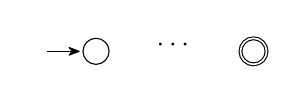
\begin{tikzpicture}[
      shorten >=1pt,node distance=2cm,on grid,>={Stealth[round]},
      initial text=, every state/.style={minimum size = 0.001cm},
      ]

      \node[state,initial]            (q_0)                      {};
      \node[state, accepting]         (q_1) [right=of q_0]       {};
      \node [fit=(q_0) (q_1)] {$\cdots$};
    \end{tikzpicture}
    \caption{The NFA recognizing $\regex$}
  \end{subfigure}
  \begin{subfigure}[b]{0.49\textwidth}
    \centering
    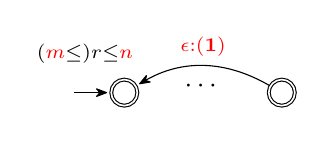
\begin{tikzpicture}[
      shorten >=1pt,node distance=2cm,on grid,>={Stealth[round]},
      initial text=, every state/.style={minimum size = 0.001cm},
      accepting text=
      ]

      \node at (-0.5,0.5) {$\scriptstyle (\myemph{m}\leq) r\leq \myemph{n}$};
      \node[state,initial,accepting]            (q_0)                      {};
      \node[state, accepting]         (q_1) [right=of q_0]       {};
      \path[->] (q_1) edge[bend right]   node    [above] {\myemph{$\scriptstyle \mathbf{\epsilon:(1)}$}} (q_0);
      \node [fit=(q_0) (q_1)] {$\cdots$};
    \end{tikzpicture}
    \caption{The CEFA recognizing $\regex^{\{m,n\}}$}
  \end{subfigure}
  \caption{The construction of counting operator}
  \label{fig:construct_repetition}
\end{figure}
\begin{example}
  To construct the CEFA recognizing $(\Sigma\setminus a)\{5,60\}$ with alphabet $\Sigma = \{a,b,c\}$. As shown in Fig.\ref{subfig:count_aut_sigma_minus_a_5_60}, the base cases are the constructions of character $b$ (Fig.\ref{subfig:count_aut_b}) and $c$ (Fig.\ref{subfig:count_aut_c}). The first inductive step is building their union (Fig.\ref{sub@subfig:count_aut_sigma_minus_a}). The second inductive step is to add counting information on the automaton. To do that we add a new register $r$ to save counting times,  transitions $q_2\xrightarrow[(1)]{\epsilon} q_0$ and $q_1\xrightarrow[(1)]{\epsilon} q_0$  to update the counting times. The accepting condition of each accepting state is $5\leq r\leq 60$, which ensures the accepting word's counting time is in the range $[5,60]$. After epsilon elimination we get the CEFA recognizing $(\Sigma\setminus a)\{5,60\}$ (shown in Fig.\ref{subfig:count_aut_sigma_minus_a_5_60}).
  \begin{figure}[h]
    \begin{subfigure}[b]{0.49\textwidth}
      \centering
      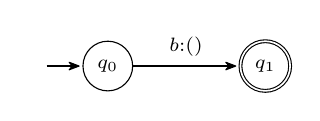
\begin{tikzpicture}[
        shorten >=1pt,node distance=2cm,on grid,>={Stealth[round]},
        initial text=, every state/.style={minimum size = 0.001cm},
        ]
        \node[state,initial]            (q_0)                      {$\scriptstyle q_0$};
        \node[state,accepting]                    (q_1) [right=of q_0]       {$\scriptstyle q_1$};

        \path[->] (q_0) edge              node      [above]           {$\scriptstyle b:()$} (q_1);
      \end{tikzpicture}
      \caption{The NFA recognizing $b$}
      \label{subfig:count_aut_b}
    \end{subfigure}
    \begin{subfigure}[b]{0.49\textwidth}
      \centering
      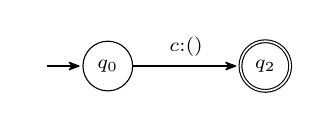
\begin{tikzpicture}[
        shorten >=1pt,node distance=2cm,on grid,>={Stealth[round]},
        initial text=, every state/.style={minimum size = 0.001cm},
        ]
        \node[state,initial]            (q_0)                      {$\scriptstyle q_0$};
        \node[state,accepting]                    (q_1) [right=of q_0]       {$\scriptstyle q_2$};

        \path[->] (q_0) edge              node      [above]           {$\scriptstyle c:()$} (q_1);
      \end{tikzpicture}
      \caption{The NFA recognizing $c$}
      \label{subfig:count_aut_c}
    \end{subfigure}
    \begin{subfigure}[b]{0.49\textwidth}
      \centering
      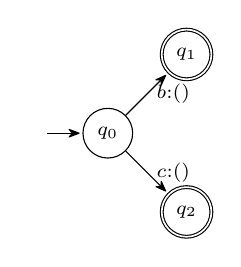
\begin{tikzpicture}[
        shorten >=1pt,node distance=1cm,on grid,>={Stealth[round]},
        initial text=, every state/.style={minimum size = 0.001cm},
        ]
        \node[state,initial]      (q_0)                      {$\scriptstyle q_0$};
        \node (q_tmp) [right=of q_0]       {};
        \node[state, accepting]   (q_1) [above=of q_tmp]       {$\scriptstyle q_1$};
        \node[state, accepting]   (q_2) [below=of q_tmp]       {$\scriptstyle q_2$};

        \path[->] (q_0) edge node [right] {$\scriptstyle b:()$} (q_1)
        (q_0) edge           node [right] {$\scriptstyle c:()$} (q_2);
      \end{tikzpicture}
      \caption{The NFA recognizing $\Sigma \setminus a$}
      \label{subfig:count_aut_sigma_minus_a}
    \end{subfigure}
    \begin{subfigure}[b]{0.49\textwidth}
      \centering
      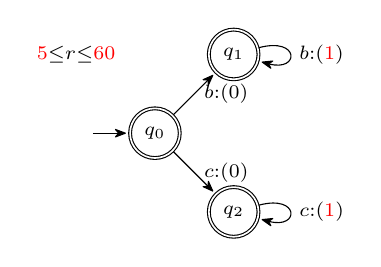
\begin{tikzpicture}[
        shorten >=1pt,node distance=1cm,on grid,>={Stealth[round]},
        initial text=, every state/.style={minimum size = 0.005cm},
        ]
        \node at (-1, 1) {$\scriptstyle \myemph{5}\leq r \leq \myemph{60}$};
        \node[state,initial, accepting]      (q_0)                      {$\scriptstyle q_0$};
        \node (q_tmp) [right=of q_0]       {};
        \node[state, accepting]   (q_1) [above=of q_tmp]       {$\scriptstyle q_1$};
        \node[state, accepting]   (q_2) [below=of q_tmp]       {$\scriptstyle q_2$};

        \path[->] (q_0) edge node [right] {$\scriptstyle b:(0)$} (q_1)
        (q_1) edge [loop right] node {$\scriptstyle b:(\myemph{1})$} (q_1)
        (q_0) edge           node [right] {$\scriptstyle c:(0)$} (q_2)
        (q_2) edge [loop right] node {$\scriptstyle c:(\myemph{1})$} (q_0);
      \end{tikzpicture}
      \caption{The CEFA recognizing $(\Sigma\setminus a)\{\myemph{5},\myemph{60}\}$}
      \label{subfig:count_aut_sigma_minus_a_5_60}
    \end{subfigure}
    \caption{The example of constructing regex with counting}
  \end{figure}
\end{example}

Above discusses the construction of handled counting operators. In the same way, we can not construct the unhandled counting operator. For example, for the regex $(ab^{\{1,100\}})*$ with unhandled counting operator, there are infinite repetitions of $ab^{\{1,100\}}$. The counting times of each repetition are irrelevant, so we can not represent them using finite registers. We must syntactically rewrite the unhandled counting operator into union and concatenation operators. More exactly, the sub-regex $\regex^{\{m,n\}}$ in the unhandled regex is rewritten into $\underbrace{\regex\cdot\regex\cdots\regex}_{m \text{ times}}\mid\cdots\mid \underbrace{\regex\cdot\regex\cdots\regex}_{n \text{ times}}$.
% Based on the decision procedure defined in the paper \cite{atva2020}, we propose an efficient algorithm to solve ESL formula $\varphi\wedge \psi$ where $\varphi$ is the conjunction of literals and $\psi$ is the conjunction of linear literals without length operation. For each string variable $x$, we first compute pre-images of all linear literal $i=|x|$. Then we generate CEFAs of all regular expressions $\regex$ in all regular literals $x\in \regex$ and intersect these CEFAs and pre-images to get the final automaton $\aut_x$ for $x$. There is a final CEFA for each string variable $x$. The linear arithmetic constraint $\psi$ restricts the accepting word of final CEFAs. Thus the satisfiability problem is the emptiness checking problem of final CEFAs under $\psi$. If it is empty, the string constraints are unsatisfiable. Otherwise, the string constraints are satisfiable.
% The emptiness checking problem of CEFAs under linear integer arithmetic is theoretically pspace-complete\cite{atva2020}. To solve it efficiently for a practical example, we develop heuristic ways such as under-approximation (Section \ref{subsec:under-approx}) and symbolic-aware simplification (Section \ref{subsec:simplify}).

%\subsection{Handling of String-length}
Given a string-length constraint, we build a CEFA with a register storing the word length. Namely, the CEFA is $(\{q_I\}, \Sigma, \{q_I\xrightarrow[(1)]{\Sigma} q_I\}, q_I, \{q_I\}, r, \theta)$ where accpeting condition $\theta$ is based on the length formula. As an illustration, example \ref{eg:pre_len} shows the CEFA of length constraints $|x| > 120$, whose language is the set of all words with a length greater than $120$. The simple loop $q_I\xrightarrow[(1)]{\Sigma} q_I$ increase $1$ on register $r$ for all char in $\Sigma$, so that the value of $r$ is equal to the length of the accepting word. The accepting condition $\theta$ attaches $q_I$ to $r > 120$, ensuring the length of the accepting word is greater than $120$.

% The formal definition of pre-images of abundant string functions is listed in \cite{atva2020}, and we do not repeat it here.
\begin{example}[The CEFA of $|x| > 120$]\label{eg:pre_len} 
  \begin{figure}[h]
    \centering
    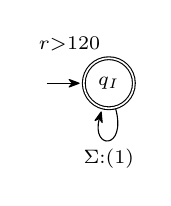
\begin{tikzpicture}[
      shorten >=1pt,node distance=2cm,on grid,>={Stealth[round]},
      initial text=, every state/.style={minimum size = 0.001cm},
      ]

      \node at (-0.5, 0.5) {$\scriptstyle r > 120$};
      \node[state,initial,accepting]            (q_0)       {$\scriptstyle q_I$};

      \path[->] (q_0) edge [loop below] node{$\scriptstyle\Sigma:(1)$} ();
    \end{tikzpicture}
  \end{figure}
\end{example} 
% \subsection{Combine Regex-counting and String-length}
% In the previous section, we discussed the construction of the regex-counting operator and string-length constraint. In this section, we show how to combine them. 
% \begin{definition} [The Product of Two CEFA]

%   Given two CEFAs $\aut_1 = (Q_1, \Sigma, \delta_1, q_{I_1}, F_1, R_1, \theta_1)$ and $\aut_2 = (Q_2, \Sigma, \delta_2, q_{I_2}, F_2, R_2, \theta_2)$ with $R_1\cap R_2 = \emptyset$, the product of them, denoted by $\aut_1 \times \aut_2$, is defined as $(Q_1\times Q_2, \Sigma, \delta, (q_{I_1}, q_{I_2}), F_1\times F_2, R_1\cup R_2, \theta)$ where
%   \begin{itemize}
%     \item $\delta$ comprises the tuples $((q_1, q_2), a, (q_1', q_2'), \myvec{v_1}\cdot \myvec{v_2})$ such that $(q_1, a, q_1', \myvec{v_1})\in \delta_1$ and $(q_2, a, q_2', \myvec{v_2})\in \delta_2$.
%     \item $\theta((q_1, q_2))$ is $\theta_1(q_1)\wedge \theta_2(q_2)$ for each accepting state $(q_1, q_2)\in F_1\times F_2$.
%   \end{itemize}
% \end{definition}
% With the help of product, we can combine the CEFAs of regex-counting and string-length. For example, the CEFA of $x$ in the string constraints $x \in (\Sigma \setminus a)^{\{5, 60\}} (\Sigma \setminus b)^{\{5, 60\}} (\Sigma \setminus c)^{\{0, 60\}} \wedge x \in \Sigma^* c \wedge |x| > 120$ is the product of the CEFA of regex $(\Sigma \setminus a)^{\{5, 60\}} (\Sigma \setminus b)^{\{5, 60\}} (\Sigma \setminus c)^{\{0, 60\}}$, the CEFA of regex $\Sigma^*$ and the CEFA of length constraints $|x| > 120$.
}
%%%%%%%%%%% original texts by denghang %%%%%
%%%%%%%%%%% original texts by denghang %%%%%

\vspace{-2mm}
\subsection{Solving $\cefadec$} \label{subsec:cefadec}
\vspace{-1mm}

In this section, we present a procedure to solve the $\cefadec$ problem: Suppose that $x_1, \cdots, x_n$ are mutually distinct string variables, $\Lambda_{x_1}, \cdots, \Lambda_{x_n}$ are nonempty sets of CEFA over the same alphabet $\Sigma$ where $\Lambda_{x_i} = \{\aut_{i, 1}, \cdots, \aut_{i, l_i}\}$ for every $i \in [n]$. Moreover, the sets of registers $R_{\aut_{1, 1}}, \cdots, R_{\aut_{n, l_n}}$ are mutually disjoint, and $\varphi$ is a LIA formula whose free variables are from $\bigcup \limits_{i \in [n], j \in [l_i]} R_{\aut_{i, j}}$. 
The procedure comprises three steps. 

\medskip
\noindent
\emph{Step 1.} For each $i \in [n]$, compute a CEFA $\cB_{i} = \aut_{i,1} \cap \cdots \cap \aut_{i, l_i}$, and let $\Lambda'_{x_i} := \{\cB_i\}$. \qed

%At first, we compute CEFA $\cB_{i} = \aut_{i,1} \cap \cdots \cap \aut_{i, l_i}$ for each $i \in [n]$. For each $i \in [n]$, let $\Lambda'_{x_i} = \{\cB_i\}$. Evidently, $R_{\cB_i}= \bigcup \limits_{j \in [l_i]} R_{\aut_{i, j}}$ for each $i \in [n]$.
After Step 1, the nonemptiness of CEFA in $\Lambda_{x_1}, \cdots, \Lambda_{x_n}$ w.r.t. $\varphi$ is reduced to the nonemptiness of CEFA in $\Lambda'_{x_1}, \cdots, \Lambda'_{x_n}$ w.r.t. $\varphi$. 

%CEFA in $\Lambda'_{x_1} = \{\cB_1\}, \cdots, \Lambda'_{x_n} = \{\cB_n\}$ are nonempty w.r.t. $\varphi$ 
%

%Therefore, to solve the nonemptiness of CEFA in $\Lambda'_{x_1} = \{\cB_1\}, \cdots, \Lambda'_{x_n} = \{\cB_n\}$ w.r.t. $\varphi$, it is sufficient to compute $\cefaout(\cB_1)$


%Since the construction of $\cB_1, \cdots, \cB_n$ involves the computation of the product of multiple CEFA, it incurs an exponential blow-up in the worst case. Therefore, it is vital to reduce the sizes of these CEFAs. In the sequel, we propose some techniques to reduce the automata sizes. 

In the following steps, we reduce the non-emptiness of CEFA in $\Lambda'_{x_1}, \cdots, \Lambda'_{x_n}$ w.r.t. $\varphi$ to the satisfiability of an LIA formula. The reduction relies on two observations: The first observation follows that $\Lambda'_{x_i}$ for each $i \in [n]$ contains exactly one CEFA, and the second observation follows that the non-emptiness of exactly one CEFA w.r.t LIA formulae is entirely unrelated to the alphabet.

\vspace{-2mm}
\begin{observation}\label{obs-cefa-output}
CEFA in $\Lambda'_{x_1} = \{\cB_1\}, \cdots, \Lambda'_{x_n} = \{\cB_n\}$ are nonempty w.r.t. $\varphi$ iff there are $\myvec{v_{1}} \in \cefaout(\cB_1), \cdots, \myvec{v_{n}} \in \cefaout(\cB_n)$ such that $\varphi[\myvec{v_{1}}/R_{\cB_{1}}, \cdots, \myvec{v_{n}}/R_{\cB_{n}}]$ is true.
\end{observation}
\vspace{-1mm}

%From the fact that $\Lambda'_{x_i}$ for each $i \in [n]$ contains exactly one CEFA, we deduce that the following two conditions are equivalent.  
%\begin{itemize}
%\item CEFA in $\Lambda'_{x_1} = \{\cB_1\}, \cdots, \Lambda'_{x_n} = \{\cB_n\}$ are nonempty w.r.t. $\varphi$, namely, 
%there are an assignment $\theta: \{x_1, \cdots, x_n\} \rightarrow \Sigma^*$ and vectors $\myvec{v_{1}}, \cdots, \myvec{v_{n}}$ such that $(\theta(x_1); \myvec{v_1}) \in \Lang(\cB_1)$, $\cdots$, $(\theta(x_n); \myvec{v_n}) \in \Lang(\cB_n)$ and $\varphi[\myvec{v_{1}}/R_{\cB_{1}}, \cdots, \myvec{v_{n}}/R_{\cB_{n}}]$ is true,
%
%\item there are $\myvec{v_{1}} \in \cefaout(\cB_1), \cdots, \myvec{v_{n}} \in \cefaout(\cB_n)$ such that $\varphi[\myvec{v_{1}}/R_{\cB_{1}}, \cdots, \myvec{v_{n}}/R_{\cB_{n}}]$ is true.
%\end{itemize}

Let $\aut = (R, Q, \Sigma, \delta, I, F, \alpha)$ be a CEFA and $\costset_\aut = \{\myvec{v} \mid \exists q, a, q'.\ (q, a, q', \myvec{v}) \in \delta\}$. 
Moreover, let $\cU_\aut = (Q, \costset_\aut, \delta', I, F)$ be an NFA over the alphabet $\costset_\aut$ that is obtained from $\aut$ by dropping the accepting condition and ignoring the characters, that is, $\delta'$ comprises tuples $(q, \myvec{v}, q')$ such that $(q, a, q', \myvec{v}) \in \delta$ for $a \in \Sigma$.
%Then $\cefaout(\aut) = \parikh(\NFA')$.
%

\vspace{-2mm}
\begin{observation}\label{obs-cefa-nfa}
For each CEFA $\aut = (R, Q, \Sigma, \delta, I, F, \alpha)$, 
%
$$\cefaout(\aut) = \left\{\sum \limits_{\myvec{v} \in \costset_\aut} \eta(\myvec{v}) \myvec{v} \  \big{|}\ \eta \in \parikh(\cU_\aut) \mbox{ and }  \alpha\left[ \sum \limits_{\myvec{v} \in \costset_\aut} \eta(\myvec{v}) \myvec{v} \big{/} R \right] \mbox{ is true}\right\}.$$
%
\end{observation}
\vspace{-1mm}


For $i \in [n]$, let $\alpha_i$ be the accepting condition of $\cB_i$. 
Then from Observation~\ref{obs-cefa-nfa}, we know that the following two conditions are equivalent, 
\begin{itemize}
%\item CEFA in $\Lambda'_{x_1} = \{\cB_1\}, \cdots, \Lambda'_{x_n} = \{\cB_n\}$ are nonempty w.r.t. $\varphi$, namely, 
%there are an assignment $\theta: \{x_1, \cdots, x_n\} \rightarrow \Sigma^*$ and vectors $\myvec{v_{1}}, \cdots, \myvec{v_{n}}$ such that $(\theta(x_1); \myvec{v_1}) \in \Lang(\cB_1)$, $\cdots$, $(\theta(x_n); \myvec{v_n}) \in \Lang(\cB_n)$ and $\varphi[\myvec{v_{1}}/R_{\cB_{1}}, \cdots, \myvec{v_{n}}/R_{\cB_{n}}]$ is true,
%
\item there are $\myvec{v_{1}} \in \cefaout(\cB_1), \cdots, \myvec{v_{n}} \in \cefaout(\cB_n)$ such that $\varphi[\myvec{v_{1}}/R_{\cB_{1}}, \cdots, \myvec{v_{n}}/R_{\cB_{n}}]$ is true, 
%CEFA in $\Lambda'_{x_1} = \{\cB_1\}, \cdots, \Lambda'_{x_n} = \{\cB_n\}$ are nonempty w.r.t. $\varphi$ 
%
\item 
there are $\eta_1 \in \parikh(\cU_{\cB_1}), \cdots, \eta_n \in \parikh(\cU_{\cB_n})$ such that 
%
%\begin{equation}\label{eqn-cefa-lia}
\[
\bigwedge \limits_{i \in [n]} \alpha_i\left[ \sum \limits_{\myvec{v} \in \costset_{\cB_i}} \eta_i(\myvec{v}) \myvec{v} \big{/}R_{\cB_i}  \right] \wedge \varphi \left[\sum \limits_{\myvec{v} \in \costset_{\cB_1}} \eta_1(\myvec{v}) \myvec{v} \big{/}R_{\cB_1}, \cdots, \sum \limits_{\myvec{v} \in \costset_{\cB_n}} \eta_n(\myvec{v}) \myvec{v} \big{/}R_{\cB_n} \right]
\]
%\end{equation} 
%
is true. 
\end{itemize}

Therefore, to solve the nonemptiness of CEFA in $\Lambda'_{x_1}, \cdots, \Lambda'_{x_n}$ w.r.t. $\varphi$, it is sufficient to compute the existential LIA formulas $\psi_{\cU_{\cB_1}}(\fZ_{\costset_{\cB_1}}), \cdots, \psi_{\cU_{\cB_n}}(\fZ_{\costset_{\cB_n}})$ to represent the Parikh images of $\cU_{\cB_1}$, $\cdots$, $\cU_{\cB_n}$ respectively, where $\fZ_{\costset_{\cB_i}} = \{\anivarz_{i,\myvec{v}} \mid \myvec{v} \in \costset_{\cB_i}\}$ for $i \in [n]$, and solve the satisfiability of the following existential LIA formula
%
%\begin{equation}\label{eqn-cefa-lia}
\[
\begin{array}{l}
%\scriptsize
\bigwedge \limits_{i \in [n]} \left(\psi_{\cU_{\cB_i}}(\fZ_{\costset_{\cB_i}}) \wedge \alpha_i\left[\sum\limits_{\myvec{v} \in \costset_{\cB_i}} \anivarz_{i, \myvec{v}} \myvec{v} \big{/}R_{\cB_i}  \right] \right)\  \wedge \\
\ \ \varphi \left[ \sum\limits_{\myvec{v} \in \costset_{\cB_1}} \anivarz_{1, \myvec{v}} \myvec{v} \big{/}R_{\cB_1}, \cdots, \sum\limits_{\myvec{v} \in \costset_{\cB_n}} \anivarz_{n, \myvec{v}} \myvec{v} \big{/}R_{\cB_n} \right].
\end{array}
\]
%\end{equation}
Intuitively, the integer variables $\anivarz_{i, \myvec{v}}$ represent the number of occurrences of $\myvec{v}$ in the strings accepted by $\cU_{\cB_i}$.
%where $\anivarz_{\myvec{v}}$'s are integer variables to represent the number of occurrences of $\myvec{v}$. 

Because the sizes of the LIA formulas $\psi_{\cU_{\cB_1}}(\fZ_{\costset_{\cB_1}}), \cdots, \psi_{\cU_{\cB_n}}(\fZ_{\costset_{\cB_n}})$ are proportional to the sizes (more precisely, the alphabet size, the number of states and transitions) of NFA $\cU_{\cB_1}, \cdots, \cU_{\cB_n}$, and the satisfiability of existential LIA formulas is NP-complete, it is vital to reduce the sizes of these NFA to improve the performance.

Since
$\sum \limits_{\myvec{v} \in \costset(\cB_i)} \eta(\myvec{v}) \myvec{v} = \sum \limits_{\myvec{v} \in \costset(\cB_i) \setminus \{\myvec{0}\}} \eta(\myvec{v}) \myvec{v}$ for each $i \in [n]$ and $\eta \in \parikh(\cU_{\cB_i})$, it turns out that 
the $\myvec{0}$-labeled transitions in $\cU_{\cB_i}$ do not contribute to the final output $\sum \limits_{\myvec{v} \in \costset(\cB_i)} \eta(\myvec{v}) \myvec{v}$. Therefore, we propose the following simplification technique for the NFA $\cU_{\cB_i}$'s. 

\medskip
\noindent
\emph{Step 2.} For each $i \in [n]$, we view the transitions $(q, \myvec{0}, q')$ in $\cU_{\cB_i}$ as $\varepsilon$-transitions $(q, \varepsilon, q')$, and remove the $\varepsilon$-transitions from $\cU_{\cB_i}$. Then we determinize and minimize the resulting NFA.   \qed

For $i \in [n]$, let  $\cC_i$ denote the DFA obtained from $\cU_{\cB_i}$ by executing Step 2 and $\costset_{\cC_i} := \costset_{\cB_i} \setminus \{\myvec{0}\}$. From the construction, we know that $\parikh(\cC_i) = \prj_{\costset_{\cC_i}}(\parikh(\cU_{\cB_i}))$ for each $i \in [n]$.
Therefore, we compute LIA formulas from $\cC_i$'s, instead of $\cU_{\cB_i}$'s, to represent the Parikh images. 

\medskip
\noindent
\emph{Step 3.} For each $i \in [n]$, we compute an existential LIA formula $\psi_{\cC_i}(\fZ_{\costset_{\cC_i}})$ from $\cC_i$ to represent $\parikh(\cC_i)$. Then we solve the satisfiability of the following formula,
%
\vspace{-1mm}
\[
\begin{array}{l}
\bigwedge \limits_{i \in [n]} \left(\psi_{\cC_i}(\fZ_{\costset_{\cC_i}}) \wedge \alpha_i\left[\sum\limits_{\myvec{v} \in \costset_{\cC_i}} \anivarz_{i, \myvec{v}} \myvec{v} \big{/}R_{\cB_i}  \right] \right) \ \wedge \\
\ \ \varphi \left[ \sum\limits_{\myvec{v} \in \costset_{\cC_1}} \anivarz_{1, \myvec{v}} \myvec{v} \big{/}R_{\cB_1}, \cdots, \sum\limits_{\myvec{v} \in \costset_{\cC_n}} \anivarz_{n, \myvec{v}} \myvec{v} \big{/}R_{\cB_n} \right].
\end{array}
\]
\vspace{-1mm}
\qed
%\[
%\bigwedge \limits_{i \in [n]} \psi_{\cC_i}(\fZ_{\costset_{\cB_i}}) \wedge 
%\varphi \left[ \sum\limits_{\myvec{v} \in \costset_{\cB_1}} \anivarz_{\myvec{v}} \myvec{v} \big{/}R_{\cB_1}, \cdots, \sum\limits_{\myvec{v} \in \costset_{\cB_n}} \anivarz_{\myvec{v}} \myvec{v} \big{/}R_{\cB_n} \right].
%\]

% Finally, although we propose techniques to reduce the sizes of $\cU_{\cB_i}$'s, it is still relatively expensive to compute LIA formulas from $\cC_i$'s and solve their satisfiability, especially for those satisfiable problem instances, namely, those instances where CEFA in $\Lambda_{x_1}, \cdots, \Lambda_{x_n}$ are nonempty w.r.t. $\varphi$.   
% Therefore, in the sequel, we propose a heuristic to search for solutions by utilizing under approximations, to be executed before Step 3. Intuitively, we search for solutions by bounding the lengths of the strings that are accepted by $\cC_i$'s. The heuristic uses a constant bound $B > 0$ and searches for solutions incrementally, starting from strings of length $0$. Since the heuristic is executed after Step 2 and before Step 3, we call it Step 2.5. 

% For $i \in [n]$, suppose $R_{\cB_i} = (r_{i,1},\cdots, r_{i, k_i})$ and $\cC_i = (Q'_i, \costset_{\cC_i}, \delta'_i, q_{i,0}, F'_i)$. 

% \paragraph*{Step 2.5.} Initially, let $len := 0$, and for each $i \in [n]$, let 
% %$\confset_{\cC_i}:=\emptyset$, 
% $\confset_{\cC_i}:=\{(q_{i,0}, \myvec{0})\}$ 
% and $\psi_{\cC_i}:= \lfalse$.  Then iterate the following procedure until $len = B+1$.
% \begin{enumerate}
% \item Let $\xi: = \bigwedge \limits_{i \in [n]} \alpha_i \wedge \varphi$.
% %
% \item For each $i \in [n]$, do the following.
% \begin{enumerate}
% \item Let 
% %$\confset_{\cC_i}:= \confset_{\cC_i} \cup \confset'_{\cC_i}$, 
% $old_i:=\confset_{\cC_i}$, $\confset_{\cC_i}:=\emptyset$.
% %
% \item For each $(q, \myvec{v}) \in old_i$,
% \begin{enumerate}
% \item if $q \in F'_i$, then let $\psi_{\cC_i}:=\psi_{\cC_i} \vee (\bigwedge \limits_{j \in [k_i]} r_{i,j} = v_j)$, 
% %
% %\item let $\confset'_{\cC_i}:=\confset'_{\cC_i} \setminus \{(q, \myvec{v})\}$, 
% %
% \item for each $(q, \myvec{v'}, q') \in \delta'_i$, let $\confset_{\cC_i}:=\confset_{\cC_i} \cup \{(q', \myvec{v}+ \myvec{v'})\}$. 
% \end{enumerate}
% %
% %\item 
% %
% \item Let $\xi := \xi \wedge \psi_{\cC_i}$. 
% \end{enumerate}
% %
% \item If $\xi$ is satisfiable, then report $\ltrue$ and the whole algorithm terminates. 
% %
% \item Let $len: = len+1$. $\blacksquare$
% \end{enumerate}
% Intuitively, for each $i \in [n]$, $\psi_{\cC_i}$ is a global variable whose value is never reset, and it stores the set of ``final'' valuations of registers of $\cC_i$ (that is, the valuations obtained when reaching final states), and $\confset_{\cC_i}$ stores the set of newly discovered (not necessarily final) ``configurations'' of $\cC_i$.
% %, and $\confset_{\cC_i}$ stores those that have been discovered before. 
% Note that the solution searching algorithm in Step 2.5 is incremental because when the value of $len$ is incremented, the searching continues from $\confset_{\cC_i}$'s, not from scratch.
%, whose values are not reset.
%Furthermore, for each $i \in [n]$, we can remove the redundancy of characters/vectors in $\cC_i$. 



%%%%%%%%%%%% the original texts by Denghang %%%%%%%%%
%%%%%%%%%%%% the original texts by Denghang %%%%%%%%%
\hide{
Moreover, the transitions $(q, \myvec{0}, q')$ in $\cC_i$ can be seen as $\varepsilon$-transitions, that is, we can replace each transition $(q, \myvec{0}, q')$ with $(q, \varepsilon, q')$, without affecting the set $\{ \sum\limits_{\myvec{v} \in V_i} m_{\myvec{v}} \myvec{v} \mid \myvec{m} \in parikh(\cC_i)\}$. Therefore, we first do these replacements and apply the $\varepsilon$-transition removal procedure. Then we utilize the determinization and minimization algorithm for NFA to reduce the size of $\cC_i$. 

It turns out that to solve the non-emptiness of CEFA in $\Lambda'_{x_1} = \{\cB_1\}, \cdots, \Lambda'_{x_n} = \{\cB_n\}$ w.r.t. $\varphi$. We can ignore the characters in $\cB_1,\cdots, \cB_n$ because there is only one CEFA for each string variable, and $\varphi$ only cares about the values of registers.

%When the characters in $\cB_1, \cdots, \cB_n$ are ignored, they can be seen as NFAs. 
For each $i \in [n]$, let $\cC_i$ be the automaton obtained from $\cB_i$ by replacing each transition $(q, a, q', \myvec{v})$ with $(q, \myvec{v}, q')$. 
Then for each $i \in [n]$, $\cC_i$ can be seen as an NFA over the alphabet $V_i$, where $V_i$ is the set of vectors $\myvec{v}$ occurring in the transitions $(q, a, q', \myvec{v})$ of $\cB_i$. 

Then the set of costs output by $\cB_i$, that is, $\{\myvec{v} \mid (w; \myvec{v}) \in \Lang(\cB_i)\}$ can be reduced to the computation of the Parikh image of $\cC_i$, namely, 
%
$$\{ \sum\limits_{\myvec{v} \in V_i} m_{\myvec{v}} \myvec{v} \mid \myvec{m} \in parikh(\cC_i)\}.$$

Moreover, the transitions $(q, \myvec{0}, q')$ in $\cC_i$ can be seen as $\varepsilon$-transitions, that is, we can replace each transition $(q, \myvec{0}, q')$ with $(q, \varepsilon, q')$, without affecting the set $\{ \sum\limits_{\myvec{v} \in V_i} m_{\myvec{v}} \myvec{v} \mid \myvec{m} \in parikh(\cC_i)\}$. Therefore, we first do these replacements and apply the $\varepsilon$-transition removal procedure. Then we utilize the determinization and minimization algorithm for NFA to reduce the size of $\cC_i$. 

Finally, if there are two indices $1 \le i' < j' \le |R_{\cB_i}|$ such that $v_{i'} = v_{j'}$ for each vector $\myvec{v} \in V_i$, then we can remove the $j'$-th component from the characters (vectors) of $\cC_i$, and let $\varphi := \varphi \wedge r_{i, i'} = r_{i, j'}$. By abusing the notation, we still use $\cC_i$ to denote the resulting NFA. 

By doing this, we reduce the automata sizes. Then we compute an LIA formula $\psi_{i}$ from $\cC_i$ to specify the Parikh images of $\cC_i$. Then the nonemptiness of $\cB_1, \cdots, \cB_n$ w.r.t. $\varphi$ is reduced to the satisfiability of $\psi_1 \wedge \cdots \psi_n \wedge \varphi$.

under approximation

In summary, we obtain an algorithm for solving the non-emptiness of $\Lambda_{x_1}, \cdots, \Lambda_{x_n}$ w.r.t. $\varphi$, as illustrated in Figure~\ref{xxx}. 

\zhilin{stopped here}

After encoding counting operator and length constraint to CEFAs, there are only automaton memberships $x\in \aut$ and LIA formula $t_1 \ \op \ t_2$ where $\aut$ is CEFA and $t_1, t_2$ are integer terms. Let $\psi$ denotes the conjunction of all LIA formulae $t_1\ \op\ t_2$ and $\Lambda_x = \{\aut_x^1, \aut_x^2,\cdots \aut_x^n\}$ denotes the set of CEFAs in the automaton membership $x\in \aut$. The emptiness checking problem of $\Lambda_x$ under $\psi$ is the problem that checks whether there exists a word $w$ such that $w\in \aut_x^1, w\in \aut_x^2\cdots w\in \aut_x^n$ and $\psi[\myvec{V}/\myvec{r}]$ holds, where $\myvec{r}$ are all registers and $\myvec{V}$ are corresponding register values in automata of $\Lambda_x$ after running $w$. The emptiness problem is \emph{abbreviated as $SAT_{CEFA}[LIA]$ problem}. 

As mentioned in \cite{atva2020}, the \emptinessprob{} is theoretically Pspace-complete. In previous work, we have used a model-checking tool \emph{nuXmv}\cite{nuxmv} to solve it. However, it needs to be more efficient for complex string constraints. So we put forward a new framework that brings in symbolic-aware simplification and under-approximation heuristics.

The main idea of our framework is to simplify the input CEFAs firstly and under-approximate the solution of the \emptinessprob{} by adding length bounds on string variables. If the under-approximation is satisfiable, the CEFAs are not empty under $\psi$. Otherwise, we check the Parikh image of the simplified CEFAs. If the Parikh image is satisfiable, the CEFAs are not empty under $\psi$. Alternatively, they are empty. The framework is \emph{sound} and \emph{complete}.

The framework is shown in Algorithm \ref{alg:emptiness}. We simplify the input CEFAs at line 1 because they may have too many transitions and registers to solve. The main idea of the simplification is treating the alphabet as unary and the symbolic updates as characters of transitions in the minimization. After the simplification, we try to find a solution by under-approximation at line 2 and line 3. The under-approximation algorithm explores possible satisfiable register values within a length bound $MaxBound$. We return true if it finds a solution because the under-approximation is sound for sat. Otherwise, we compute the Parikh images of the simplified CEFAs and check if the Parikh images are satisfiable in conjunction with $\psi$ at line 12. The Parikh image checking is complete so that satisfiability implies non-emptiness directly. 

The under-approximation program is incremental. In other words, it first tries to find a solution with a smaller length bound of each string variable and increments the string length bound if the search for a smaller length bound fails. $MaxBound$ is the max length bound we try, empirically set to $15$ in our experiment. It should not be too large because of the exponential growth of searching space. The details of simplification and under-approximation are shown in Algorithm \ref{alg:simplify}, and the details are shown in Algorithm \ref{alg:underApprox}.

\begin{algorithm}[h]
  \caption{ $\algfun{nonEmpty}(auts, \psi)$}
  \label{alg:emptiness}
  \begin{algorithmic}[1]
    \Require the CEFAs $auts$ and the linear integer arithmetic $\psi$
    \Ensure $true$ or $false$
    \Statex
    \State $simpliAuts \leftarrow \algfun{simplify}(auts)$
    % \For{$bound \gets 1, MaxBound$ }
    % \State $\varphi_{under}\gets \algfun{underApprox}(simpliAuts, bound)$
    % \If{$\varphi_{under}\wedge \psi$ is sat}
    % \State \textbf{return} $true$
    % \EndIf
    % \EndFor
    \If{\algfun{underApproxSolve}($simpliAuts, \psi, MaxBound$) is true}
    \State \textbf{return} $true$
    \EndIf
    \State $\varphi \gets \algfun{parikhImage}(simpliAuts)$
    \If{$\varphi\wedge \psi$ is sat}
    \State \textbf{return} $true$
    \Else
    \State \textbf{return} $false$
    \EndIf
  \end{algorithmic}
\end{algorithm}
\subsubsection{Symbolic-Aware Simplification} \label{subsec:simplify}
The purpose of simplification is to remove duplicated transitions and registers. In the emptiness checking Algorithm \ref{alg:emptiness}, the non-emptiness equals the reachability of CEFAs. The symbolic updates on transitions are meritorious because it influences register values, while the characters are not. The alphabet of the CEFA can be ignored (i.e., the alphabet is $\{a\}$), and the vectors can be seen as characters. The special vector $\myvec{0}_n$ with only zero elements is seen as a $\epsilon$ character since it does not change the values of registers. Namely, given a CEFA $\aut = (Q, \Sigma, \delta, q_I, F, R, \theta)$, we obtain a symbolic NFA  $\aut_{sym} = (Q, \Sigma', \delta', q_I, F)$ where
\begin{itemize}
  \item $\Sigma' = \{\myvec{v} \mid \text{there exists one transition in } \aut \text{ with update } \myvec{v}\}$,
  \item the transition set $\delta'$ is composed of transition $q\xrightarrow{\myvec{v}}q'$ if there is a transition $q\xrightarrow[\myvec{v}]{b} q'$ in $\delta$.
\end{itemize}

 For the symbolic NFA $\aut_{sym}$, we treat $q\xrightarrow{\myvec{0}_n} q'$ as an epsilon transition since it does not change the values of the registers. Then we apply the epsilon elimination algorithm \cite{aut_hopcraft} to delete these epsilon transitions. After that, we apply the determination and minimization algorithm \cite{aut_hopcraft} of NFAs to $\aut_{sym}$, resulting in a smaller automaton $\aut_{simp}$. Finally, we reinterpret $\aut_{simp}$ as a CEFA with the accepting condition of $\aut$ and unary alphabet $\Sigma = \{a\}$. Above illustrates functions $\algfun{determinizeByVec}$ and $\algfun{minimizeByVec}$ from line 3 to line 5. From line 6 to line 14, we check whether two registers $r_i$ and $r_j$ are duplicated. (i.e., the symbolic updates of them are always the same). If they are duplicated at line 6, we remove one of them and the corresponding symbolic update from line 8 to line 10. After deleting the duplicated registers, we add constraint $r_i = r_j$ to store the value of the deleted register at line 12, ensuring that the value of the deleted register is consistent.

We have the following proposition:
\begin{proposition}
  Given a set of CEFAs $\Lambda=\{\aut_1, \cdots, \aut_2\}$ and arbitrary LIA $\psi$, the emptiness of $\Lambda$ on $\psi$ is equal to the emptiness of $\algfun{simplify}(\Lambda)$ on $\psi$.
\end{proposition}
\begin{algorithm}[h]
  \caption{$\algfun{simplify}(auts)$}
  \label{alg:simplify}
  \begin{algorithmic}[1]
    \Require A set of CEFAs
    \Ensure The simplified CEFAs
    \Statex
    \For{$\aut \in auts$}
    \State Suppose that $\aut = (Q, \Sigma, \delta, q_I, F,
      R, \theta)$ and $R=(r_1,\cdots, r_n)$
    \State $\algfun{epsilonElimByVec}(\aut)$
    \State $\algfun{determinizeByVec}(\aut)$
    \State $\algfun{minimizeByVec}(\aut)$
    \ForAll{$(i, j)$ where $1\leq i \leq j \leq n$}
    \If {$\myvec{v}[i] = \myvec{v}[j]$ for every vector $\myvec{v}\in \aut$ }
    \State $R\gets(\cdots r_{j-1}r_{j+1}\cdots)$ \Comment remove $r_j$ from the register vector $R$
    \ForAll{$\myvec{v'}\in \aut$}
    \State $\myvec{v'}\gets(\cdots\myvec{v'}[j-1]\myvec{v'}[j+1]\cdots)$ \Comment remove $\myvec{v'}[j]$ from each vector $\myvec{v'}$
    \EndFor
    \State $\theta \gets\theta\wedge r_i = r_j$
    \EndIf
    \EndFor
    \EndFor
    \State \textbf{return} $auts$
  \end{algorithmic}
\end{algorithm}
\begin{example}
  Considering the CEFA (Fig.\ref{subfig:count_aut_sigma_minus_a_5_60}) recognizing $(\Sigma\setminus a)\{1,60\}$ where $\Sigma = \{a,b,c\}$. We first obtain a symbolic NFA of it by ignoring the unary alphabet (Fig.\ref{subfig:sigma_minus_a_5_60:simplify}). Then we eliminate epsilon transitions $q_0\xrightarrow[]{(0)} q_1$ and $q_0\xrightarrow[]{(0)}q_2$, resulting in the minimized NFA directly. Finally, we reinterpret it as CEFA by adding accepting condition $1\leq r \leq 60$(Fig.\ref{subfig:simp_final}).
  \begin{figure}[h]
    \begin{subfigure}[b]{0.49\textwidth}
      \centering
      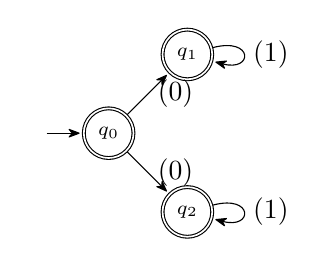
\begin{tikzpicture}[
        shorten >=1pt,node distance=1cm,on grid,>={Stealth[round]},
        initial text=, every state/.style={minimum size = 0.005cm},
        ]
        % \node at (-1, 1) {$\scriptstyle 5\leq r \leq 60$};
        \node[state,initial, accepting]      (q_0)                      {$\scriptstyle q_0$};
        \node (q_tmp) [right=of q_0]       {};
        \node[state, accepting]   (q_1) [above=of q_tmp]       {$\scriptstyle q_1$};
        \node[state, accepting]   (q_2) [below=of q_tmp]       {$\scriptstyle q_2$};

        \path[->] (q_0) edge node [right] {$(0)$} (q_1)
        (q_1) edge [loop right] node {$(1)$} (q_1)
        (q_0) edge           node [right] {$(0)$} (q_2)
        (q_2) edge [loop right] node {$(1)$} (q_0);
      \end{tikzpicture}
      \caption{The symbolic NFA of $\aut_{\Sigma\setminus a\{5,60\}}$}
      \label{subfig:sigma_minus_a_5_60:simplify}
    \end{subfigure}
    \begin{subfigure}[b]{0.49\textwidth}
      \centering
      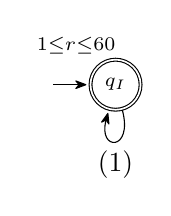
\begin{tikzpicture}[
        shorten >=1pt,node distance=1cm,on grid,>={Stealth[round]},
        initial text=, every state/.style={minimum size = 0.001cm},
        ]

        \node at (-0.5, 0.5) {$\scriptstyle 1\leq r \leq 60$};
        \node[state,initial,accepting]            (q_0)       {$\scriptstyle q_I$};
  
        \path[->] (q_0) edge [loop below] node{$(1)$} ();
      \end{tikzpicture}
      \caption{Simplify the CEFA based on symbolic label}
      \label{subfig:simp_final}
    \end{subfigure}
    \caption{Symbolic simplification removes duplicated transitions and states.}
    \label{fig:simplification_example}
  \end{figure}

\end{example}
\begin{example}
  Considering the string constraints $i=|x|\wedge j=|x|$. We compute the CEFAs of $i=|x|$, $j=|x|$ and intersect them to get the final CEFA represented in Fig.\ref{subfig:duplicate}. However, the register $r_1$ and $r_2$ in the final CEFA are duplicated since their symbolic updates are always the same. We simplify the CEFA by removing the duplicated register $r_2$ and corresponding symbolic updates, as shown in Fig.\ref{subfig:remove_duplicate}. To maintain the value of $r_2$, we add a constraint $r_2=r_1$ in the accepting condition.
  \begin{figure}[h]
    \begin{subfigure}[b]{0.49\textwidth}
      \centering
      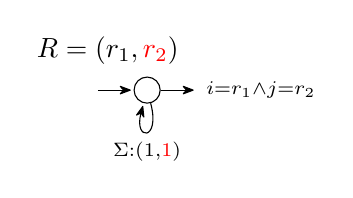
\begin{tikzpicture}[
        shorten >=1pt,node distance=1cm,on grid,>={Stealth[round]},
        initial text=, every state/.style={minimum size = 0.001cm},
        accepting text=${\scriptstyle i=r_1\wedge j=r_2 }$, accepting/.style=accepting by arrow,
        ]
        \node at (-0.5,0.5) {$R=(r_1, \myemph{r_2})$};
        \node[state,initial,accepting]            (q_0)       {};

        \path[->] (q_0) edge [loop below] node{$\scriptstyle\Sigma:(1,\myemph{1})$} ();
      \end{tikzpicture}
      \caption{An automaton with duplicated registers}
      \label{subfig:duplicate}
    \end{subfigure}
    \begin{subfigure}[b]{0.49\textwidth}
      \centering
      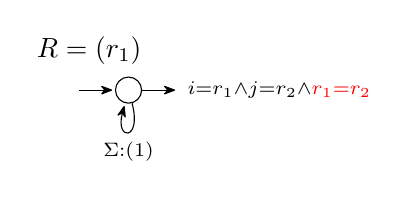
\begin{tikzpicture}[
        shorten >=1pt,node distance=1cm,on grid,>={Stealth[round]},
        initial text=, every state/.style={minimum size = 0.001cm},
        accepting text=${\scriptstyle i=r_1\wedge j=r_2\wedge \myemph{r_1 = r_2} }$, accepting/.style=accepting by arrow,
        ]

        \node at (-0.5,0.5) {$R=(r_1)$};
        \node[state,initial,accepting]            (q_0)       {};

        \path[->] (q_0) edge [loop below] node{$\scriptstyle\Sigma:(1)$} ();
      \end{tikzpicture}
      \caption{Remove the duplicated registers and corresponding symbolic updates}
      \label{subfig:remove_duplicate}
    \end{subfigure}
    \caption{Symbolic simplification removes duplicated registers.}
    \label{fig:duplicate}
  \end{figure}

\end{example}

\subsubsection{Under-Approximation} \label{subsec:under-approx}
The purpose of under-approximation is to accelerate the solving process of satisfiable instances. With the observation that the accepted string words in practical instances are usually short, we under-approximate the \emptinessprob{} by adding length bounds on string variables. The LIA formula representing possible register value is incrementally generated based on the incremental length bounds, and this section discusses its implementation details. The main idea is to create an LIA formula enumerating all possible values of registers in accepting runs within some length bounds. More detailed, The enumeration is carried out from low to high length bounds, in which the end states and registers' values of the last enumeration are maintained and used in the following enumeration. Although the number of possible runs is an exponential growth of the bound, we usually solve practical satisfiable instances within 1s because the lengths of strings in the solution are generally less than 5.

As shown in the Algorithm \ref{alg:underApprox}, $\varphi_{under}$ is the under-approximated LIA formula which is initialized to the input LIA formula $\psi$ at line 2. $\varphi_\aut$ is the under-approximated LIA formula of each automaton $\aut$ which is initialized to $false$ at line 3. $lastStates$ maps each automaton $\aut$ to the set consisting of pairs of state and corresponding registers' value in the last enumeration. $lastStates(\aut)$ is initialized to the pair of the initial state and zero values for each automaton $\aut$ at line 4. $length$ is the current bound of lengths of string variables which is initialized to $0$ at line 5. The main loop at lines 6-20 iteratively tries possible solutions from low to high length bound. For each iteration, we generate the LIA formula respectively for each automaton. To each CEFA $\aut$, we get pairs of last state and corresponding registers' values from $lastStates$ at line 8. If the last state is accepted at line 9 in each pair, we add the LIA formula of the possible registers' values to $\varphi_\aut$ as a conjunct at line 10. After that, we update the set of pairs in $lastStates$ by removing the probed pair at line 12 and adding new pairs of the next state and corresponding registers' values at line 13. Finally, we combine the incremental LIA formula of each automaton at line 15. If the LIA formula $\varphi\wedge \theta$ is satisfiable at line 17, i.e., we find a solution with all strings having length less than or equal to $length$, we return \emph{true} at line 18. Otherwise, the next iteration would be invoked with a larger length. If we can not find a solution within the max string length bound, we return \emph{false} at line 22.
\begin{algorithm}[h]
  \caption{$\algfun{underApproxSolve}(auts, bound, \psi)$}
  \label{alg:underApprox}
  \begin{algorithmic}[1]
    \Require $auts$: the CEFAs, $bound$: the max string length bound, $\psi$: the LIA formula constraining the CEFAs
    % \Ensure The linear integer arithmetic $\varphi_{under}$ representing under-approximation of the register values of $auts$
    \Ensure \emph{true} if finding a solution, \emph{false} otherwise
    \Statex
    \State $\theta$ is the conjunction of all accepting conditions of $auts$
    \State $\varphi_{under}$ is an incremental LIA formula as under approximation, initialized to $\psi$
    \State $\varphi_\aut$ is an incremental LIA formula for each automaton $\aut$, initialized to $false$
    \State $lastStates(\aut)$ is the set of (last state, vector's sum) pairs of $\aut$, initialized to $\{(q_I, 0_n)\}$ 
    \State $length$ is the current bound for string-length, initialized to $0$
    \While {$length \leq bound$}
      \For{$\aut \in auts$}
        \For{$(q, \myvec{V}) \gets lastStates(\aut)$}
          \If{$q\in F$}
            \State $\varphi_{\aut} \gets \varphi_{\aut}\vee \bigwedge\limits_{i\in[1,m]} r_i = \myvec{V}[i]$
          \EndIf
          \State Remove $(q, \myvec{V})$ from $lastStates(\aut)$
          \State Add $(q', \myvec{V}+\myvec{v})$ to $lastStates(\aut)$ for each transition $q\xrightarrow[\myvec{v}]{a} q'\in \aut$
        \EndFor
        \State $\varphi_{under}\gets \varphi_{under}\wedge\varphi_\aut$
      \EndFor
      \If{$\varphi_{under}\wedge \theta$ is satisfiable}
        \State \textbf{return} \emph{true}
      \EndIf
      \State $length \gets length + 1$
    \EndWhile
    \State \textbf{return} \emph{false}
    % \For{$\aut \in auts$}
    % \State $\varphi_\aut\gets false$ 
    % \State Suppose $\aut = (Q, \Sigma, \delta, q_I, F, (r_1, \cdots, r_m), \theta)$
    % \ForAll{run $q_0q_1\cdots q_{n}$ whose length is less than $bound$}
    % \If{$q_{n}\in F$}
    % \State Let $\myvec{V}$ to be the sum of the vectors on the run
    % \State $\varphi_{\aut} \gets \varphi_{\aut} \vee(\theta(q_n)\bigwedge\limits_{i\in[1,m]} r_i = \myvec{V}[i])$
    % \EndIf
    % \EndFor
    % \State $\varphi_{under} \gets \varphi_{under}\wedge \varphi_{\aut}$
    % \EndFor
    % \State \textbf{return} $\varphi_{under}$
  \end{algorithmic}
\end{algorithm}
\begin{example}
  Consider the automaton $\aut$ in Fig. \ref{fig:overview:product:reduced} again without the LIA constraint $r_0 > 120$, i.e., $\theta$ changes to $1\leq r_1\leq 60\wedge 1\leq r_2 \leq 60\wedge 0\leq r_3 \leq 60 $. The solution of the Parikh image of it leads to a complete but inefficient result since the quantifier-free LIA formulas are solved in exponential time. Under-approximation can accelerate the solving process. In the first iteration of under-approximation, the pairs in the $lastStates(\aut)$ is the initial pair $(q_0', (0,0,0,0))$ and $\varphi_\aut$ maintains false at line 9 because $q_0'$ is not accepted. Then we update $lastStates(\aut)$ by removing the pair $(q_0', (0,0,0,0))$ and adding pairs $(q_0', (1,1,0,0)), (q_1', (1,0,1,0)), (q_2', (1,0,0,0))$. In the second iteration, $\varphi_\aut$ changes to $r_0=1\vee r_1=0\vee r_2=0\vee r_3 = 0$ because $q_2'$ is accepted. $\varphi_{under}$ is always equal to $\varphi_\aut$ since there is only one automaton. We solve the formula $\theta\wedge \varphi_{under}$ and find it is unsatisfiable. In the third iteration, the pairs in the $lastStates(\aut)$ with accepting state should be $(q_0', (2,2, 0, 0)), (q_1', (2,1,1,0))$, $(q_1', (2,0,2,0))$, $(q_2', (2,1,0,0)), (q_2', (2,0,1,0)),$ $(q_2', (2,0, 0, 0))$. The corresponding registers' values for the accepted state $q_2'$ are $(2,1,0,0), (2, 0, 1, 0), (2, 0, 0, 0)$, in which the value of $r_1$ and $r_2$ can not be both larger than 1 which is required by $\theta$. So the formula $\theta\wedge \varphi_{under}$ is still unsatisfiable. Finally, We obtain a pair $(q_2', (3,1,1,0))$ from the pair $(q_1', (2,1,1,0))$ and the transition $q_1'\xrightarrow[(1,0,0,0)]{} q_2'$, whose corresponding registers' values is a solution $(3,1,1,0)$, i.e., $r_0=3, r_1=1, r_2=1, r_3=0$.
\end{example}

\subsection{High-level algorithm}

The pseudocode presented in Algorithm \ref{alg:high} outlines the framework of our solving process. We construct the automata of all length operations occurring in the ESL conjunction $\varphi$ at line 3 and the automata of all regular memberships at line 4. In the following steps, we call an automaton to be \emph{final} if we will not operate it anymore. The set $finalAuts$ contains all final automata for all string variables and is initially empty at line 1. The intersection of $\aut_{len}$ and $\aut_{regex}$ at line 5 ensures the final automaton of $x$ reserves both length and regular information. At line 6, we compute an NFA form to throw unsat rapidly. An NFA form of CEFA is obtained by removing update functions and accepting conditions while maintaining graph structure. More exactly, given a CEFA $\aut = (Q,\Sigma, \delta, q_I, F, R, \theta)$, the NFA form of $\aut$ is $(Q, \Sigma, \delta', q_I, F)$ where $\delta'$ is composed of transition $q\xrightarrow[]{a} q'$ for $q\xrightarrow[\myvec{v}]{a} q'\in \delta$. The NFA form is an over-approximation of the CEFA, so that unsat is directly thrown if we find the NFA form is already empty at line 7. Sometimes the over-approximation is useful. For example, to solve the string constraint $x\in \Sigma_{/a}\{1,300\}\wedge x\in \Sigma^*a\Sigma^* $ which CVC5 has failed on, the NFA form is empty because there is no path to accepting states. 

After obtaining all final CEFAs of all string variables and their NFA forms are not empty, we check whether the final CEFAs are empty under the linear integer arithmetic $\psi$ at line 12. If they are empty under $\psi$, we return $unsat$. Otherwise, we return $sat$.

\begin{algorithm}[h]
  \caption{High-level algorithm}
  \label{alg:high}
  \begin{algorithmic}[1]
    \Require Conjunction of literals $\varphi$ and conjunction of linear literals $\psi$
    \Ensure \emph{sat} or \emph{unsat}
    \Statex
    \State $finalAuts \leftarrow \emptyset$
    \ForAll{string variables $x$ occurring in $\varphi$}
    \State $\aut_{len} \leftarrow$ intersection of all pre-images of $i=|x|$ in $\varphi$
    \State $\aut_{regex} \leftarrow$ intersection of all CEFAs of $x \in \regex$ in $\varphi$
    \State $\aut_x \leftarrow$ intersection of $\aut_{len}$ and $\aut_{regex}$
    \State $\aut_{nfa} \leftarrow$ NFA form of $\aut_x$
    \If{$\aut_{nfa}$ is empty}
    \State \textbf{return} \emph{unsat}
    \EndIf
    \State $finalAuts \leftarrow finalAuts \cup \{\aut_x\}$
    \EndFor
    \If{$\algfun{isEmpty}(finalAuts, \psi)$ }
    \State \textbf{return} \emph{unsat}
    \Else
    \State \textbf{return} \emph{sat}
    \EndIf
  \end{algorithmic}
\end{algorithm}
}
%%%%%%%%%%%% the original texts by Denghang %%%%%%%%%
%%%%%%%%%%%% the original texts by Denghang %%%%%%%%%



%\end{document}

\section{Optimizations for non-register-representable RECL Constraints} \label{sec:heuristic}
%!TEX root = ../main.tex

In Section~\ref{sec:algorithm}, to deal with the non-register-representable RECL constraints, we unfold all the non-register-representable occurrences of counting operators. Nevertheless, 
the naive unfolding incurs an exponential blow-up over the formula sizes, especially when the counting bounds are large. 
Recall that an occurrence of counting operators is said to be non-register-representable if it is in the scope of some Kleene star, another counting operator, complement, or language difference. Since Kleene star can be seen as a special case of the counting operators, and language difference $e_1 \setminus e_2$ can be rewritten as $e_1 \cap \overline{e_2}$, without loss of generality, we can assume that a non-register representable occurrence of a counting operator is in the scope of another counting operator or some complement operator. 
In the sequel, to alleviate the formula-size blow-up problem resulted from the naive unfolding, we present various optimizations, for the nesting of counting operators and the nesting of counting operators and a complement operator respectively. 
% two situations that a counting operator is in the scope of another counting operator and in the scope of a complement operator respectively. 

\subsection{Optimizations for the nesting of counting operators}\label{heuristic:nested}

In the sequel, we propose an optimization for the nesting of counting operators. 
The optimization is designed for the special case that the nesting depth of counting operators is one. For a RECL constraint whose nesting depth of counting operators is greater than two, we can apply the optimization for the inner-most nesting of counting operators and decrement the nesting depth, then apply the optimization again to the resulting constraint, and continue this process, until obtaining a register-representable RECL constraint.  

The main idea of the optimization is illustrated by the constraint $x \in (a^{\{1,1000\}})^{\{1,2\}}$. If we apply the naive unfolding in Section~\ref{sec:algorithm}, we will unfold  $a^{\{1,1000\}}$ and obtain the constraint $x \in (a(\varepsilon + a + aa + \cdots + \underbrace{a\cdots a}_{999}))^{\{1,2\}}$. It is easy to observe that a smarter way is to unfold  $^{\{1,2\}}$, instead of $^{\{1, 1000\}}$. If we do this, then we get a constraint $x \in (a^{\{1,1000\}})(\varepsilon + a^{\{1,1000\}})$, whose size is much smaller, compared to $x \in (a(\varepsilon + a + aa + \cdots + \underbrace{a\cdots a}_{999}))^{\{1,2\}}$. (Recall that we assume a binary encoding of the integer constants in counting operators.)

Let us describe the optimization more precisely. 
\begin{itemize}
\item For a regular expression $e = (e_1)^{\{m,n\}}$ where $e_1$ is a register-representable regular expression, we can unfold the counting operators in the following ways to obtain a register-representable RECL constraint: (i) unfold the counting operators in $e_1$, (ii) unfold the counting operator $^{\{m,n\}}$. 
%
Let $\ufld_1(e)$ and $\ufld_2(e)$ denote the resulting regular expressions. 

\item We estimate the sizes of the two CEFAs $\aut_{\ufld_1(e)}, \aut_{\ufld_2(e)}$ constructed from $\ufld_1(e), \ufld_2(e)$ respectively as pairs $(\snum_1(e), \rnum_1(e))$ and $(\snum_2(e), \rnum_2(e))$, where $\snum_1(e)$ and $\rnum_1(e)$ are the estimates of the number of states and registers in $\aut_{\ufld_1(e)}$, similarly for $\snum_2(e)$ and $\rnum_2(e)$. 
%
\item From the construction in Section~\ref{sec:algorithm}, 
two NFAs $\cU_{\aut_{\ufld_2(e)}}, \cU_{\aut_{\ufld_2(e)}}$ are constructed from $\aut_{\ufld_1(e)}$ and $\aut_{\ufld_2(e)}$ by dropping the accepting conditions and ignoring the characters. As a result, the alphabets of $\cU_{\aut_{\ufld_2(e)}}, \cU_{\aut_{\ufld_2(e)}}$ are the set of integer vectors  $\myvec{v}$ occurring in the transitions of $\aut_{\ufld_1(e)}, \aut_{\ufld_2(e)}$ respectively. The integer vectors of  $\aut_{\ufld_1(e)}$ are of form $(\underbrace{0, \cdots, 0}_{i-1}, 1, \underbrace{0, \cdots, 0}_{r'-i-1})$, where $i \in [r']$. Consequently, the size of the alphabet of $\cU_{\aut_{\ufld_1(e)}}$ is bounded by $\rnum_1(e)$. Similarly for $\cU_{\aut_{\ufld_1(e)}}$. 
Finally, we estimate the sizes (number of transitions) of the NFAs $\cU_{\aut_{\ufld_1(e)}}, \cU_{\aut_{\ufld_2(e)}}$ as $sz_1 = (\snum_1(e))^2 \cdot \rnum_1(e)$ and $sz_2 = (\snum_2(e))^2 \cdot \rnum_2(e)$ respectively.
%
\item If $sz_1 \le sz_2$, then we choose to unfold the counting operators in $e_1$. Otherwise, we choose to unfold the counting operator $^{\{m,n\}}$. 
\end{itemize}

%In the sequel, we show how we estimate the sizes of CEFAs constructed from register-representable regular expressions. 

It remains to show how to compute the pairs $(\snum_1(e), \rnum_1(e))$ and $(\snum_2(e), \rnum_2(e))$ from $e=(e_1)^{\{m,n\}}$. Let $e=(e_1)^{\{m,n\}}$ be a regular expression where $e_1$ is a register-representable regular expression. Then we compute $\snum'_1(e_1)$ and $(\snum'_2(e_1), \rnum'_2(e_1))$ by a structural induction on $e_1$. Finally, let $(\snum_1(e), \rnum_1(e)) = (\snum'_1(e_1), 1)$ and $(\snum_2(e), \rnum_2(e)) = (\snum'_2(e_1), \rnum'_2(e_1))$.
\begin{itemize}
  \item If $e_1 = \emptyset$ or $e_1 = \epsilon$, then $\snum'_1(e_1)  = 0$ and $(\snum'_2(e_1), \rnum'_2(e_1))  = (0, 0)$. 
%
 %
  \item If $e_1 = e_2 \concat e_3$, then $\snum'_1(e_1) = \snum'_1(e_2) + \snum'_1(e_3)$ and 
%
  $$
  \begin{array}{l }
 (\snum'_2(e_1), \rnum'_2(e_1)) =  \\
  \ \ \ \ (n(\snum'_2(e_2) + \snum'_2(e_3)), n(\rnum'_2(e_2) + \rnum'_2(e_3))).
 \end{array}
  $$
%
 \item If $e_1 = e_2 + e_3$, then $\snum'_1(e_1) = \snum'_1(e_2) + \snum'_1(e_3)$ and 
%
  $$
  \begin{array}{l }
 (\snum'_2(e_1), \rnum'_2(e_1)) =  \\
  \ \ \ \ (n(\snum'_2(e_2) + \snum'_2(e_3)), n(\rnum'_2(e_2) + \rnum'_2(e_3)+1)).
 \end{array}
  $$
 (Recall that the construction of $\aut_1 \cup \aut_2$ introduces one additional register.)
%
 \item If $e_1 = e_2 \cap e_3$, then $\snum'_1(e_1) = \snum'_1(e_2) \times \snum'_1(e_3)$ and 
%
  $$
  \begin{array}{l }
 (\snum'_2(e_1), \rnum'_2(e_1)) =  \\
  \ \ \ \ (n(\snum'_2(e_2) \times \snum'_2(e_3)), n(\rnum'_2(e_2) + \rnum'_2(e_3))).
 \end{array}
  $$
%
 \item If $e_1 = \overline{e_2}$, then $\snum'_1(e_1) = 2^{\snum'_1(e_2)}$ and 
%
  $
%  \begin{array}{l }
 (\snum'_2(e_1), \rnum'_2(e_1)) =  (n \cdot 2^{\snum'_2(e_2)}, 0).
% \end{array}
  $
 (The exponential blow-up is explained by the fact that the determinization is needed for the complementation.) 
%
%  \item If $\regex = \overline{\regex_1}$, then $s_\regex = 2^{s_{\regex_1}}$ (since the determinization is needed for the complement) and $r_\regex = 0$.
%
 \item If $e_1 = (e_2)^*$, then $\snum'_1(e_1) = \snum'_1(e_2)$ and 
%
  $
%  \begin{array}{l }
 (\snum'_2(e_1), \rnum'_2(e_1)) =  (n \snum'_2(e_2), 0).
% \end{array}
  $
%  \item If $\regex = \regex_1^*$, then $s_{\regex} = s_{\regex_1}$ and $r_{\regex} = 0$.
%  \item $\regex = \regex_1 \backslash \regex_2$ can be transferred to $\regex = \regex_1 \cap \overline{\regex_2}$ and then the size can be computed by the formula of $\cap$ and $\bar{}$.
 \item If $e_1 = (e_2)^{\{m', n'\}}$ or $e_1 = (e_2)^{\{n', \infty\}}$, then $\snum'_1(e_1) = n' \snum'_1(e_2)$ and 
%
  $
%  \begin{array}{l }
 (\snum'_2(e_1), \rnum'_2(e_1)) =  (n \snum'_2(e_2), n).
% \end{array}
  $
%  \item For $\regex = \regex_1^{\{m, n\}}$ or $\regex = \regex_1^{\{n,\infty\}}$, $s_{\regex} = s_{\regex_1}$ and $r_{\regex} = 1$.
\end{itemize}

%The naive approach for nested counting in the paper \cite{Denghang2023} is to unwind all inner counting operators. This approach may generate a large number of states, which is linear to the product of the counting bounds in regex and exponential to the length of the regex. For example, naive unwinding regex $(a^{\{1,1000\}})^{\{1,2\}}$ generate a CEFA containing 1000 states. But if we only unwind the outer counting operator of the regex, not the inner, we obtain a CEFA containing only 2 states. The side effect is that we need two registers to store the information of counting in the inner regex (unwinding of the outer counting operator repeats the inner regex, which also repeats the registers of the inner regex). We present a heuristic to reduce the number of states generated by the unwinding process. The idea is to unwind the counting operator with less bound and fewer side effects firstly. We present the heuristic in the following algorithm.

%%%%%%%%%%%%%%%%%%%%%%%%%%%%%%%%%%
%%%%%%%%%%%%%%%%%%%%%%%%%%%%%%%%%%
\hide{
\medskip
\noindent
\emph{Step 1. (Compute the number of states generated by each counting operator if we unwind it).}

For a regex $\regex$, we can approximate the number of states $size(\regex)$ generated by the following formula: 
\begin{itemize}
  \item If $\regex = \emptyset$ or $\regex = \epsilon$, then $size(\regex) = 0$. 
  \item If $\regex = \regex_1 \cdot \regex_2$ or $\regex = \regex_1 + \regex_2$, then $size(\regex) = size(\regex_1) + size(\regex_2)$.
  \item If $\regex = \regex_1^*$, then $size(\regex) = size(\regex_1)$.
  \item If $\regex = \regex_1 \cap \regex_2$, then $size(\regex) = size(\regex_1)*size(\regex_2)$.
  \item If $\regex = \overline{\regex_1}$, then $size(\regex) = 2^{size(\regex_1)} + 1$.
  \item $\regex = \regex_1 \backslash \regex_2$ can be transferred to $\regex = \regex_1 \cap \overline{\regex_2}$ and then the size can be computed by the formula of $\cap$ and $\bar{}$.
  \item For $\regex = \regex_1^{\{n,m\}}$ or $\regex = \regex_1^{\{m,\infty\}}$, $size(\regex)$ is equal to $m*size(\regex_1)$ if it is unwinded, and $size(\regex_1)$ otherwise.
\end{itemize}

For each counting operator $^{\{n,m\}}$ or $^{\{m,\infty\}}$ with $\regex$ as its subregex, the number of states generated by it is $m*size(\regex)$ if we unwind it.

The formula above is an approximation of the states of CEFA generated by Thompson's construction. Note that the number of states is linear to the bound for the counting operator.

\medskip
\noindent
\emph{Step 2. (Compute the number of registers generated by each counting operator if we unwind it).}

We unwind the counting operator with less bound first. The reason is that the number of states generated by the counting operator is linear to its bound. If we unwind the counting operator with less bound first, the number of states generated by the unwinding process is less. However, the hardness of solving the $\cefadec$ problem is not only relevant to the number of states, but also the number of registers. For a regex $\regex$, we can approximate the number of registers $reg(\regex)$ generated by the following formula:
\begin{itemize}
  \item If $\regex = \emptyset$, $\regex = \epsilon$, $\regex = \regex_1^*$ or $\regex = \overline{\regex_1}$, then $reg(\regex) = 0$.
  \item If $\regex = \regex_1\cdot \regex_2$ or $\regex = \regex_1 \cap \regex_2$, then $reg(\regex) = reg(\regex_1) + reg(\regex_2)$.
  \item If $\regex = \regex_1 + \regex_2$, then $reg(\regex) = reg(\regex_1) + reg(\regex_2) + 1$.
  \item $\regex = \regex_1 \backslash \regex_2$ can be transferred to $\regex = \regex_1 \cap \overline{\regex_2}$ and then the number of registers can be computed by the formula of $\cap$ and $\bar{}$.
  \item For $\regex = \regex_1^{\{n,m\}}$ or $\regex = \regex^{\{m, \infty\}}$, $reg(\regex)$ is equal to $m*reg(\regex_1)$ if it is unwinded, and $1$ otherwise.
\end{itemize}

For each counting operator $^{\{n,m\}}$ or $^{\{m,\infty\}}$ with $\regex$ as its subregex, the number of registers generated by it is $m*reg(\regex)$ if we unwind it.

\medskip
\noindent
\emph{Step 3. (Unwind the counting operator with less bound and fewer registers first).}

In the above two steps, we compute the number of states and registers generated by each counting operator. In some cases, we can unwind the counting operator with less bound and fewer registers directly. But in most cases, there are multiple counting operators where one counting operator has less bound and another counting operator has fewer registers. To consider the number of states and registers at the same time, we can compute the score of each counting operator by the following formula:
\begin{itemize}
  \item $score(\regex) = size(\regex) * (reg(\regex)+1)$.
\end{itemize} 
The reason why we use the product to combine the two factors is that the hardness of the $\cefadec$ problem is highly relevant to the number of variables in the final existential LIA formula, which is linear to the product of the number of states and the number of registers. Using $reg(\regex) + 1$ not $reg(\regex)$ is because the number of registers may be $0$.We unwind the counting operator with the smallest score first. 

\begin{example}
 Consider the regex $(a^{\{1,1000\}})^{\{1,2\}}$. The score of $^{\{1,1000\}}$ is $1000*(0+1) = 1000$ and the score of $^{\{1,2\}}$ is $2*(2+1) = 6$. We unwind the outer counting operator first and obtain a CEFA containing only two states.  
\end{example}
}
%%%%%%%%%%%%%%%%%%%%%%%%%%%%%%%%%%
%%%%%%%%%%%%%%%%%%%%%%%%%%%%%%%%%%



\subsection{Optimizations for the nesting of counting operators and a complement operator}

As mentioned in Section~\ref{sec:algorithm}, if some counting operators are in the scope of a complement operator, it is necessary to unfold these counting operators before the complement operation. The exponential blow-up in the unfolding combined with the blow-up in the complement operation will produce a huge number of states. To alleviate this problem, we propose two approximations of the complement operation, i.e., an under-approximation and an over-approximation, and combine them into a procedure that achieves a nice balance between efficiency and precision. 

Let $e = \overline{e_1}$ be a regular expression, where $e_1$ is a register-representable regular expression. 

\paragraph*{Under-approximation}
%
One way of doing the complement operation is to transform $e_1$ into a regular expression that does not contain counting operators. We compute an under-approximation of $e$ by replacing each occurrence of the counting operators in $e_1$, say $(e_2)^{\{m,n\}}$ or $(e_2^{\{n, \infty\}})$, by $e_2^*$. Let us use $e'_1$ to denote the resulting regular expression. Note that $e'_1$ does not contain counting operators. Moreover, it is easy to observe that $\Lang(e_1) \subseteq \Lang(e'_1)$. As a result, we have $\Lang(\overline{e'_1}) \subseteq \Lang(\overline{e_1})$. That is, $\overline{e'_1}$ is an under-approximation of $\overline{e_1}$. 

%The under-approximation is replacing each counting operator in the subregex of complement with a Kleene star operator. The language of the subregex is a superset of the language of it after under-approximation. In sequential, the complement of the subregex is a subset of the origin. Note that this approach only works for non-nested complement, which means there is no other complement operators in the complement. For nested complement,  we naively handle the inner complement operators as paper \cite{Denghang2023} and then under-approximate the outer complement operator.

\paragraph*{Over-approximation}
For $e = \overline{e_1}$, we utilize the CEFA constructed from $e_1$, say $\aut_{e_1}$, to construct a CEFA $\cB$ of $e$ so that $\Lang(\cB)$ is an over-approximation of $\Lang(e)$. 
Let $\aut_{e_1} = (R, Q, \Sigma, \delta, I, F, \alpha)$. The main idea of the construction is explained as follows: If a string $w$ is not accepted by $\aut_{e_1}$, then either there are no runs of $\aut_{e_1}$ on $w$, or every run of $\aut_{e_1}$ on $w$ stop at a non-final state or enter a final state but do not satisfy the accepting condition $\alpha$. We shall construct a CEFA $\cB$ that accepts when one of these situations occurs. Then $\overline{\Lang(\aut_{e_1})} \subseteq \Lang(\cB)$, that is, $\cB$ is an over-approximation of $e$. 

Without loss of generality, we can assume that there are no transitions out of $F$ in $\aut_{e_1}$. If this is not the case, then a new state $q_f$ can be introduced to transform $\aut_{e_1}$ into a CEFA satisfying this constraint, where $q_f$ is the unique accepting state. 
Then we define $\cB= (R \cup \{r'\}, Q \cup \{q_s\}, \Sigma, \delta', I, Q \cup \{q_s\}, \alpha')$, where
\begin{itemize}
  \item $r'$ is a new register not in $R$, 
  \item $q_s$ is a new state not in $Q$,
  \item $\delta'$ comprises the following transitions, 
  \begin{itemize}
    \item $(q, a, q', (\vec{v}, 0))$ such that $(q, a, q', \vec{v}) \in \delta$ and $q' \not \in F$,
%
    \item $(q, a, q_s,(\vec{0}, 0))$ such that there do \emph{not} exist $a$-labeled transitions out of $q$, that is, for every $q'$ and $\vec{v}$, we have $(q, a, q', \vec{v}) \not\in \delta$,
%
    \item $(q, a, q', (\vec{v}, 1))$ such that $(q, a, q', \vec{v}) \in \delta$ and $q' \in F$,
%
    \item $(q_s, a, q_s, (\vec{0}, 0))$ such that $a \in \Sigma$, 
  \end{itemize}
  \item $\alpha'$ is defined as $r' = 1 \rightarrow \neg \alpha$.
\end{itemize}
Intuitively, $q_s$ is a sink state that deals with the situations where there are no runs, and $r'$ is a register newly introduced so that the different cases of the non-accepting runs of $\aut_{e_1}$ can be captured by a single accepting condition $\alpha'$. 

Note that $\cB$ is a strict over-approximation of $e = \overline{e_1}$ since $\aut_{e_1}$ may be nondeterministic. For instance, if there are two runs of $\aut_{e_1}$ on a string $w$, say one run that ends at a non-final state and another run that ends at a final state and satisfies accepting condition $\alpha$. Then $w \in \Lang(\aut_{e_1})$, thus $w \not \in \Lang(\overline{\aut_{e_1}})$. Nevertheless, according to the construction, $w$ is accepted by $\cB$, witnessed by the run of $\aut_{e_1}$ that ends at a non-final state. 

%As we mentioned in the above section \ref{heuristic:nested}, the unwinding process of the complement operator is exponential to the counting bounds in the worst case. We present a heuristic to reduce the number of states generated by the unwinding process. The idea is to under-approximate and over-approximate the language of the regex first, so that we can avoid unwinding counting operators in complement. We present the heuristic in the following algorithm.

%%%%%%%%%%%%%%%%%%%%%%%%%%%%%%%%%%%%%
%%%%%%%%%%%%%%%%%%%%%%%%%%%%%%%%%%%%%
\hide{
\medskip
\noindent
\emph{Step 1. (Under-approximate the language of the regex with complement operators).}

The under-approximation is replacing each counting operator in the subregex of complement with a Kleene star operator. The language of the subregex is a superset of the language of it after under-approximation. In sequential, the complement of the subregex is a subset of the origin. Note that this approach only works for non-nested complement, which means there is no other complement operators in the complement. For nested complement,  we naively handle the inner complement operators as paper \cite{Denghang2023} and then under-approximate the outer complement operator.

\medskip
\noindent
\emph{Step 2. (Over-approximate the language of the regex with complement operators).}

The over-approximation is to "complement" the CEFA of the subregex directly, without unwinding the counting operators in the subregex. The over-approximated complementary algorithm for CEFA is as follows:

Given a CEFA $\aut = (R, Q, \Sigma, \delta, I, F, \alpha)$, the over-approximated complement of it is a tuple $(R\cup\{r\}, Q\cup\{s,f\}, \Sigma, \delta', I, (Q\cup\{s,f\})\backslash F, \alpha')$, where :
\begin{itemize}
  \item $r$ is a new regesiter not in $R$.
  \item $s$ and $f$ are two new states not in $Q$.
  \item $\delta'$ is a transitions set containing all transitions in $\delta$ and transitions from each state $q$ in $Q$ to $s$ with label $a$ if there is no transitions from $q$ to any state with label $a$ in $\aut$. To be more detailed, $\delta'$ is the union of four sets:
  \begin{itemize}
    \item $\{(q, a, q',(\vec{v}, 0)) \mid (q, a, q', \vec{v})\in \delta\}$
    \item $\{(q, a, s,(\vec{0}, 0)) \mid \forall q'\in Q,\vec{v}. (q, a, q', \vec{v})\not\in \delta\}$
    \item $\{(q, a, f,(\vec{v}, 1)) \mid \exists q'\in F, (q, a, q', \vec{v})\in \delta\}$
    \item $\{(s, \Sigma, s, (\vec{0}, 0))\}$
  \end{itemize}
  \item $\alpha'$ is $r \not= 1\vee \neg \alpha$
\end{itemize}

$r$ is the register used to check whether the accepted state is also accepted in the original CEFA. $s$ is the self-loop state accepting all strings that are not accepted by the original CEFA. $f$ is the merged accepted state of the original CEFA. If there is a transition $(q, a, q', \vec{v})$ terminating at the accepted state $q'$ in the original CEFA, we add a corresponding transition $(q, a, f, (\vec{v}, 1))$ in the over-approximated complement. From the definition of $\delta'$, we can see that only the transitions goto $f$ increase the value of register $r$. The value of $r$ is $1$ if and only if the accepted state is also accepted in the original CEFA. With the above construction, the meaning of the accepting condition $\alpha'$ is obvious: If the string terminates at the accepting state in the original CEFA, then the accepting condition $\alpha$ is false.

\begin{theorem}
 The language of over-approximated complement of CEFA is a superset of the language of exact complement.
\end{theorem}
\begin{proof}
 Suppose that the original CEFA is $\aut = (R, Q, \Sigma, \delta, I, F, \alpha)$, the over-approximated complement of it is $\overline{\aut}_{over} = (R\cup\{r\}, Q\cup\{s,f\}, \Sigma, \delta', I, (Q\cup\{s,f\})\backslash F, \alpha')$, and the exact complement of it is $\overline{\aut}$. To prove the theorem, we only need to show that if a string is accepted by $\overline{\aut}$, then it is accepted by $\overline{\aut}_{over}$. In other words, we need to show that if a string is not accepted by $\overline{\aut}_{over}$, then it is not accepted by $\overline{\aut}$, which means it is accepted by $\aut$. We prove it by construction.
   
 In the definition of CEFA in section \ref{sec:automaton}, a run $q_0 \xrightarrow[\myvec{\overline{v}_1}]{a_1} q_1 \cdots q_{n-1}\xrightarrow[\myvec{\overline{v}_n}]{a_n} q_n$ is \emph{accepting} by $\overline{\aut}_{over}$ if $q_n \in (Q\cup\{s,f\})\backslash F$ and $\alpha'(\myvec{\overline{v}'}/(R\cup\{r\}))$ is true, where $\myvec{\overline{v}'} = \sum \limits_{j \in [n]} \myvec{\overline{v}_j}$. If a string is not accepted by $\overline{\aut}_{over}$, then each run of the string is not accepting run, which means the run terminates at state $q\in F$ or the accepting condition $\alpha'(\myvec{\overline{v}'}/(R\cup\{r\}))$ is $false$. 
   
 If each run teminates at state $q_f\in F$, suppose that each is of form $q_0\xrightarrow[(\myvec{v_1},\myvec{0})]{a_1}q_1\cdots q_{n-1}\xrightarrow[(\myvec{v_n},\myvec{0})]{a_n}q_f$, where $\myvec{\overline{v}_i}$ is $(\myvec{v_i}, \myvec{0})$ or $(\myvec{v_i}, \myvec{1})$ for $1\leq i\leq n$. Then there is a transition $(q_{n-1}, a_n, q_f, \myvec{v_n})$ in $\delta$ because there is a transition $(q_{n-1}, a_n, q_f, (\myvec{v_n}, \myvec{0}))$ in $\delta'$. So there is a transition $(q_{n-1}, a_n, f, (\myvec{v_n}, \myvec{1}))$ in $\delta'$ based on our construction for $\delta'$. The run $q_0\xrightarrow[(\myvec{v_1},\myvec{0})]{a_1}q_1\cdots q_{n-1}\xrightarrow[(\myvec{v_n},\myvec{1})]{a_n}f$ teminates at the accepting state $f$, contridicting the assumption. 
   
 If each run makes the accepting condition $\alpha'(\myvec{\overline{v}'}/(R\cup\{r\}))$ false, then the negation of the accepting condition $\neg\alpha'(\myvec{\overline{v}'}/(R\cup\{r\}))$ is true. The negation can be rewriten to $(r=1\wedge \alpha)(\myvec{\overline{v}'}/(R\cup\{r\})) = (r=1)(\myvec{\overline{v}'}/(R\cup\{r\}))\wedge \alpha(\myvec{\overline{v}'}/(R\cup\{r\}))$. In our construction, only the transitions terminate at $f$ increase one to the value of $r$, so that the run must end at $f$ to make $r=1$ be true. $\alpha(\myvec{\overline{v}'}/(R\cup\{r\})) = \alpha(\myvec{v'}/R)$ is also need to be true, implying that the run is an accepting run of $\aut$.
\end{proof}
}
%%%%%%%%%%%%%%%%%%%%%%%%%%%%%%%%%%%%%
%%%%%%%%%%%%%%%%%%%%%%%%%%%%%%%%%%%%%

\section{Optimizations for model generation}\label{sec-opt-sol-gen}

Recall that in Section~\ref{sec:algorithm}, the satisfiability of the original RECL constraint is reduced to the satisfiability of the existential LIA formula
\[
\begin{array}{l}
\bigwedge \limits_{i \in [n]} \left(\psi_{\cC_i}(\fZ_{\costset_{\cC_i}}) \wedge \alpha_i\left[\sum\limits_{\myvec{v} \in \costset_{\cC_i}} \anivarz_{i, \myvec{v}} \myvec{v} \big{/}R_{\cB_i}  \right] \right) \ \wedge \\
\ \ \varphi \left[ \sum\limits_{\myvec{v} \in \costset_{\cC_1}} \anivarz_{1, \myvec{v}} \myvec{v} \big{/}R_{\cB_1}, \cdots, \sum\limits_{\myvec{v} \in \costset_{\cC_n}} \anivarz_{n, \myvec{v}} \myvec{v} \big{/}R_{\cB_n} \right].
\end{array}
\]
Let us use $\theta$ to denote this formula. 
Then we utilize some SMT solver, say Z3, to solve the satisfiability of $\theta$. If Z3 reports ``sat'', then it also returns a model, namely, an assignment $\amodel$ of natural numbers to the free integer variables in $\theta$. Then we utilize $\amodel$ to generate a model $\amodel'$ of the original RECL constraint $\varphi$, i.e., an assignment of strings to the string variables so that $\varphi$ is evaluated to true under $\amodel'$. 

Note that for each $i \in [n]$, the free variables $\fZ_{\costset_{\cC_i}}$ in $\theta$ correspond to the number of occurrences of characters in $\costset_{\cC_i}$, i.e. the alphabet of the NFA $\cC_i$. Moreover, recall that in $\cC_i$, the characters are just the integer vectors and the characters in the original CEFAs $\cB_i$ used to construct $\cC_i$ are ignored. 
When we utilize $\amodel$ and the CEFAs $\cB_i$ to generate $\amodel'$, for each $i \in [n]$, we record the remaining occurrences of vectors $\myvec{v}$ in the transitions of the CEFAs $\cB_i$ as a number $\nvec_{i, \myvec{v}}$ and
each time when a transition $(q, a, q', \myvec{v})$ in $\cB_i$ is traversed, $\nvec_{i, \myvec{v}}$ is decremented. Note that initially $\nvec_{i, \myvec{v}}$ is set to $\amodel(\anivarz_{i, \myvec{v}})$. The searching process terminates when $\nvec_{i, \myvec{v}}$ becomes $0$ for every $\myvec{v}$. We record the characters in the traversed transitions and obtain a string for the string variable $x_i$ when the searching process terminates. As a result, we obtain a model of $\varphi$ in the end. 

It turns out that this model generation process is inefficient, mainly due to the fact that the information about the occurrences of vectors $\myvec{v}$ in $\cB_i$ in the searching process is too coarse. In the sequel, we would like to refine this process by using the LIA formulas to obtain the information about the number of occurrences of transitions, instead of just the occurrences of integer vectors, and utilize this information to guide the search process. 
Specifically, for each $i \in [n]$ and each transition $(q, a, q', \myvec{v})$ in $\cB_i$, we introduce an integer variable $\anivarz_{i, (q, a, q', \myvec{v})}$ to denote the number of occurrences of the transition, and solve the satisfiability of the following formula,  
\[
\begin{array}{l}
\bigwedge \limits_{i \in [n]} \left(\psi_{\cC_i}(\fZ_{\costset_{\cC_i}}) \wedge \alpha_i\left[\sum\limits_{\myvec{v} \in \costset_{\cC_i}} \anivarz_{i, \myvec{v}} \myvec{v} \big{/}R_{\cB_i}  \right] \right) \ \wedge \\
\ \ \varphi \left[ \sum\limits_{\myvec{v} \in \costset_{\cC_1}} \anivarz_{1, \myvec{v}} \myvec{v} \big{/}R_{\cB_1}, \cdots, \sum\limits_{\myvec{v} \in \costset_{\cC_n}} \anivarz_{n, \myvec{v}} \myvec{v} \big{/}R_{\cB_n} \right]\ \wedge \\
\ \ \bigwedge \limits_{i \in [n]} \bigwedge \limits_{\myvec{v} \in \costset_{\cC_i}} \anivarz_{i, \myvec{v}} = \sum \limits_{(q, a, q', \myvec{v}) \mbox{ occurs in } \cB_i} \anivarz_{i, (q, a, q', \myvec{v})}.
\end{array}
\]
If an SMT solver reports that the aforementioned formula is satisfiable, then the solver can also return a model, which assigns to each variable $\anivarz_{i, (q, a, q', \myvec{v})}$ a natural number. 
%For each $i \in [n]$ and each transition $(q, a, q', \myvec{v})$ in $\cB_i$, let us use $nt_{i, (q, a, q', \myvec{v})}$ to denote the value of $\anivarz_{i, (q, a, q', \myvec{v})}$ in the model.
Then we utilize these values to generate a model (an assignment of strings to string variables) of $\varphi$. 
Let $i \in [n]$. We use a function $\lambda_i$ to record the number of occurrences of the transitions in $\cB_i$. During the search process for $\cB_i$, each time when a transition $(q, a, q', \myvec{v})$ is traversed, $\lambda_i$ is updated by decrementing $\lambda_i((q, a, q', \myvec{v}))$, moreover, $a$ is also recorded. Initially, for each $i \in [n]$ and each transition $(q, a, q', \myvec{v})$ in $\cB_i$, $\lambda_i((q, a, q', \myvec{v}))$ is set to be the value of $\anivarz_{i, (q, a, q', \myvec{v})}$ in the model. When a final state of $\cB_i$ is reached and $\lambda_i((q, a, q', \myvec{v}))$ becomes zero for each transition $(q, a, q', \myvec{v})$ in $\cB_i$, then a desired string is generated for the string variable $x_i$. 

Moreover, we propose a method to prune the search space further. Let $i \in [n]$. Suppose that during the search process for $\cB_i$, let $q$ be the current state of $\cB_i$ and $\lambda_i$ record the remaining occurrences of transitions of $\cB_i$. We compute the set of transitions of $\cB_i$ that are reachable from the state $q$. Let $\cT_q$ denote this set. If $\{(q, a, q', \myvec{c}) \mid \lambda_i((q, a, q', \myvec{c})) > 0\} \not \subseteq \cT_q$, then we know that it is impossible to continue the search process so that a string accepted by $\cB_i$ will be found and meanwhile the constraint on the number of transitions enforced by $\lambda_i$ is satisfied. Therefore, in this case, the search process for $\cB_i$ halts and is backtracked. 

%\zhilin{stopped here}

%%%%%%%%%%%%%%%%%%%%%%%%%%%%
%%%%%%%%%%%%%%%%%%%%%%%%%%%%
\hide{
In the section \ref{sec:algorithm}, we present an algorithm to solve the $\cefadec$ problem. The algorithm computes existential LIA formulas and then uses an SMT solver to solve them. However, this procedure only answers the question of whether the language of the regex is empty or not. If the language is not empty, we need to find a word in the language in practice. In our previous paper \cite{Denghang2023}, we do not explicitly present the algorithm to find a word in the language because of space limitation. We used a naive approach, which randomly searched the CEFAs by the depth-first search based on the register values obtained from solving the existential LIA formula. However, this approach is not efficient when the regexes are non-register-representable. Suppose that there are $n$ registers whose values are $r_1,\cdots, r_n$ respectively in the CEFA. We may visit each transition $O(r_1*r_2\cdots *r_n)$ times during the search. To relieve this problem, we present a heuristic to find a word in the language as follows.

\medskip
\noindent
\emph{Step 1. (Compute the transitions times visited by the accepted string of CEFAs).}

For each CEFA $\aut = (R, Q, \Sigma, \delta, I, F, \alpha)$, we already know the values of its registers after solving the existential LIA formula. The values can be seen as a constant vector of length $|R|$. We use $\myvec{R}$ to denote the vector and use $\eta((q, a, q', \myvec{v}))$ to denote the parikh image of $\aut$. Then the transition times visited by the accepted string are obtained from the following formula:
$$ \sum \limits_{(q, a, q', \myvec{v})\in \delta} \eta((q, a, q', \myvec{v}))\myvec{v} = \myvec{R}$$

\medskip
\noindent
\emph{Step 2. (Prune the search tree early by the transition times during the search process).}

After computing the transition times visited by the accepted string, we prune the search tree of the CEFA based on the transition times. The idea is that we only visit the state which is able to reach all transitions need to be visited. Other states are deleted from the CEFA so that we can reduce the search space.
Note that the transition times are updated during the search process, so the search space is reduced dynamically. The pseudo-code is presented in Algorithm~\ref{alg:findword}.

\begin{algorithm}[H]
  \caption{Find a word in the language of a CEFA}\label{alg:findword}
  \begin{algorithmic}[1]
  \Procedure{findmodel}{$\aut,tmap$}
  % \State \Comment{$tmap$ maps transition to its remaining visited times}
      \State $todo \gets Stack(\aut_{init}, tmap, '''')$
      \State $visited \gets \emptyset$
      % \State \Comment{a stack of state, remaining visited times and word}
      \While{$todo$ is not empty}
        \State $(q, tmap, w) \gets todo.pop()$
        \If{$q\in \aut_{final}$ and $tmap.values = \myvec{0}$}
          \State \Return $w$
        \EndIf
        
        \For{each transition $(q, a, q', \myvec{v})$ where $tmap[(q, a, q', \myvec{v})]>0$}
          \State $tmap'[(q, a, q', \myvec{v})] \gets tmap[(q, a, q', \myvec{v})] - 1$
          \If{$(q', tmap')\not\in visited$ \textbf{and} \textsc{isReachable}($\aut, q', tmap'$)}
            \State $todo.push((q', tmap', w\cdot a))$
            \State $visited.add((q', tmap'))$
          \EndIf
        \EndFor
      \EndWhile
      \State \Return $\emptyset$ 
  \EndProcedure
  \end{algorithmic}
  \end{algorithm}

 The procedure \textsc{findmodel} takes a CEFA $\aut$ and a transitions-times map $tmap$ as input. $tmap$ maps each transition to its remaining visited times. Stack $todo$ contains states need to be visited, their corresponding transitions-times maps and the current word. Set $visited$ is used to store the visited state with the corresponding map. $todo$ is initialized with the initial state of the CEFA, the input map $tmap$ and an empty word (line 2). $visited$ is initialized as an empty set (line 3).
 In the while loop from line 4 to line 16, the state combined with its transitions-times map is searched by the depth-first search algorithm. During the search process, the procedure returns the word if the state is an accepting state and all remaining times of transitions are $0$ (line 7). For each transition $(q, a, q', \myvec{v})$ whose remaining times are greater than $0$, the procedure decreases the remaining times by $1$ (line 10) and checks whether $(q', tmap')$ is not visited and $tmap'$ is reachable from $q'$ (line 11). We say that \textit{$tmap'$ is reachable from $q'$} if each transition $t$ with $tmap'(t)> 0$ is reachable from the state $q'$. The reachability check (Algorithm~\ref{alg:isReachable}) is vital to prune the search space and reduce the search time. If the state $q'$ is not visited and $tmap'$ is reachable from $q'$, then we push $(q', tmap', w\cdot a)$ to $todo$ and add $(q', tmap')$ to $visited$ to continue the search(line 12-13). If the while loop terminates without finding an accepting word, the procedure returns $\emptyset$ (line 17).  
  
  \begin{algorithm}[H]
    \caption{Check whether the map is reachable from the state}\label{alg:isReachable}
    \begin{algorithmic}[1]
      \Procedure{isReachable}{$\aut, q, tmap$}
      \State $todo \gets Stack(q)$
      \State $visited \gets \emptyset$
      \State $qreach \gets \emptyset$
      \While{$todo$ is not empty}
        \State $q \gets todo.pop()$
        \State $visited.add(q)$
        \For{each transition $t=(q,a,q',\myvec{v})$ where $tmap(t)>0$}
          \State $qreach.add(t)$
          \If{$q'\not\in visited$}
            \State $todo.push(q')$
          \EndIf
        \EndFor
      \EndWhile
      \State Select all transitions $t$ where $tmap(t)>0$ to set $T$
      \If{$T\subseteq qreach$}
        \State \Return \textit{true}  
      \Else 
        \State \Return \textit{false}
      \EndIf
      \EndProcedure
    \end{algorithmic}
  \end{algorithm}

 In Algorithm~\ref{alg:isReachable}, all transitions reachable from the state $q'$ are computed and saved to $qreach$. If $qreach$ covers all transitions with positive times in the input map $tmap$, then we say that $tmap$ is reachable from $q'$ and the procedure \textsc{isReachable} returns true, otherwise it returns false.  
}
%%%%%%%%%%%%%%%%%%%%%%%%%%%%
%%%%%%%%%%%%%%%%%%%%%%%%%%%%


%\vspace{-2mm}
\section{Experiments} \label{sec:implementation}
%\vspace{-2mm}
%!TEX root = ../main.tex
%\documentclass{standalone}
%\begin{document}

We implement the algorithms in Section~\ref{sec:algorithm} on top of OSTRICH~\cite{ostrich,atva2020}, resulting into\denghang{in} a version of OSTRICH called OSTRICH$^{\rm RECL}$.
Then we do experiments on two benchmark suites, to evaluate the performance of OSTRICH$^{\rm RECL}$. In the sequel, we first describe the two benchmark suites, then present the settings and results of the experiments. 

%This section presents the empirical evaluation of OstrichCEA, which is our implementation of the decision procedure introduced in Section \ref{sec:algorithm}. Our objective is to validate the effectiveness of the proposed techniques by evaluating our tool's correctness and efficiency compared to other solvers. Furthermore, we assess the efficacy of our heuristics by testing different configurations of the tool. We have implemented our encoding for counting with two heuristic algorithms on Ostrich+ \cite{atva2020}. The pre-image computation for concatenation, \verb|indexOf|, \verb|substring|, \verb|replaceAll|, \verb|reverse| and finite transducer remain unchanged. OstrichCEA is written in Scala and based on the SMT solver Princess\cite{princess}.

\subsection{Benchmark suites}

Our experiments utilize two benchmark suites, namely, AutomatArk and RegCoL. In total, there are 48,834 instances in the two benchmark suites. All the benchmark instances are in SMTLIB2 format. 

\paragraph*{AutomatArk benchmark suite.}
The AutomatArk benchmark suite is adapted from the AutomatArk suite in \cite{z3str3re} by filtering out the string constraints that contain no occurrences of counting operators and adding the length constraint $|x| > 10$ (where $x$ is a string variable). There are 8,215 instances in the AutomatArk suite here.
Note that the original AutomatArk benchmark suite in \cite{z3str3re} includes 19,979 instances in total, which are conjunctions of regular membership queries and generated out of regular expressions from \cite{automatark}. 
%Only 8,751 ones that contain counting operators out of 19,979 instances. 

\paragraph*{RegCoL benchmark suite.} There are 40,628 RECL constraints in the RegCoL suite. These constraints are generated by extracting regular expressions with counting operators from \cite{regex_lingua_franca,redos_lenka} and constructing for each regular expression $e$ a RECL constraint of the form 
$$x \in e \wedge x \in \overline{\Sigma^*(<+ >+'+''+\&)\Sigma^*} \wedge |x| > 10,$$   
where $\Sigma^*(<+ >+'+''+\&)\Sigma^*$ is a regular expression that specifies at least one occurrence of special characters $<$, $>$, $'$, $''$, or $\&$, and $\overline{e'}$ denotes the complement of a regular expression $e'$. We would like to remark that there are about 500,000 real-world regular expressions in \cite{regex_lingua_franca,redos_lenka} and regular expressions with counting operators occupy about 8\% of them. 

%%%%%%%%%%%%%%%%%% the benchmark suite written by Denghang %%%%%%%%%%%
%%%%%%%%%%%%%%%%%% the benchmark suite written by Denghang %%%%%%%%%%%
\hide{
We conducted a comparison on four sets of benchmarks based on regex with 
counting operator, consisting of a total of 49,379 instances. We analyze all 19 developed benchmarks listed in \cite{zaligvinder_2021} and find that only \textbf{AutomatArk} benchmarks have regular membership with counting operator. In total, almost 18\% of the instances we evaluated were sourced from published industrial benchmarks or other solver developers. The other instances are generated by ourselves with regular expressions from real world. Each set of the benchmark is evenly divided into "large" and "small": the "large" set contains instances with large upper bounds of counting operator (the sum of upper bounds is greater than 50), and "small" contains remained instances. About 10\% of the benchmarks are in a "large" set. More details about the benchmarks are shown below.

\subsubsection{AutomatArk} is the 8,751 instances generated by Berzish et al.\cite{z3str3re}. It is based on real-world regular expression queries from Loris D'Antoni\cite{automatark}. The origin set comprises two tracks, a simple and a hard track, with 19,979 instances. The simple track contains instances with a single regular expression membership constraint, whereas the hard track can hold up to five membership constraints for a single variable per instance. We extract 8,751 instances containing counting operator.

\subsubsection{ReDos} is the set of 1,624 instances we generated. It is based on the ReDos-attacked regular expression collected by Lenka et al. For each regular expression, we generate an instance as the template (\ref{eq:template}) where $\regex$ is the regular expression. The regular membership predicate $x\not\in \Sigma^*(<\mid >\mid '\mid ''\mid \&)\Sigma^*$ sanitizes the input string $x$ to avoid the attack. The length lower bound is set to $20$ for the "small" set and $50$ for the "large" set.

\subsubsection{RegexLib} is the set of 1,623 instances we generated similarly to the \textbf{ReDos} benchmark. It is based on the regular expressions collected by James C. Davis et al.\cite{regex_lingua_franca} from regex lib website\cite{regexlib}. The website is the Internet's first Regular Expression Library. Currently, it has indexed 4149 expressions from 2818 contributors around the world since 2001. We extract 1,623 instances containing bounded repetition from 4149 instances. The length lower bound is set to $20$ for the "small" set and $50$ for the "large" set.

\subsubsection{StackOverflow} is the 37381 instances we generated similarly to the \textbf{ReDos} benchmark. As the Regexlib benchmark, the real-world regex expressions are collected by James C. Davis et al.\cite{regex_lingua_franca} from StackOverflow website\cite{stackoverflow}. The website is a question-and-answer site for professional and enthusiast programmers. We extract 37,381 instances containing bounded repetition from almost 500,000 instances. The length lower bound is set to $20$ for the "small" set and $50$ for the "large" set.
\begin{equation} \label{eq:template}
  x\in \regex \wedge x\not\in \Sigma^*(<\mid >\mid '\mid ''\mid \&)\Sigma^*\wedge |x| > 50(or \ 20)
\end{equation}
}
%%%%%%%%%%%%%%%%%% the benchmark suite written by Denghang %%%%%%%%%%%
%%%%%%%%%%%%%%%%%% the benchmark suite written by Denghang %%%%%%%%%%%

\subsection{Experiment results}

We evaluated the performance of OSTRICH$^{\rm RECL}$ against the state-of-the-art string constraint solvers, including CVC5 
%(version 1.0.5) 
\cite{cvc5}, Z3seq \cite{z3seq}, Z3-Trau 
%(github commit 1628747) 
\cite{z3trau}, Z3str3
%(github commit 59e9c87) 
\cite{z3str3}, Z3str3RE \cite{z3str3re}, and OSTRICH\footnote{The name OSTRICH+ was used in~\cite{atva2020}, where nuXmv model checker was called to solve the nonemptiness of CEFA w.r.t. LIA. } 
%(github commit 8297d8d) 
\cite{atva2020}. All experiments are conducted on CentOS Stream release 8 with 12 Intel(R) Xeon(R) Platinum 8269CY 3.10GHz CPU cores and 190 GB memory. We use the Zaligvinder framework \cite{zaligvinder_2021} to execute the experiments, where the timeout period is set as 60 seconds per instance. 

The experiments are designed to answer the following two research questions. 
\begin{description}
\item[Q1] Does OSTRICH$^{\rm RECL}$ solve RECL constraints more efficiently than the state-of-the-art string constraint solvers ?

\item[Q2] Do the size-reduction and under-approximation techniques proposed in Section~\ref{sec:algorithm} indeed improve the performance ?
\end{description}

Q1 is answered by running OSTRICH$^{\rm RECL}$ and the aforementioned solvers on AutomatArk and RegCoL. The experimental results can be found in Table~\ref{tab:results_all}. From Table~\ref{tab:results_all}, we can see that OSTRICH$^{\rm RECL}$ solvers almost all 48,834 instances, except 144 of them, that is, it solves 48,689 instances correctly, which is 3,982/2,263/24,568/12,823/1,082/7083 more than the number of instances solved by CVC5/Z3seq/Z3-Trau/Z3str3/Z3str3RE/OSTRICH respectively. 
%    
Note that Z3seq, Z3-Trau, Z3str3, and Z3str3RE have soundness errors, where the result of CVC5 is taken as the ground truth. If CVC5 reports ``unknown'' or ``timeout'' in some instance, then no soundness errors will be reported in this instance. 
%A soundness error is reported if the result of a solver for an instance is different from CVC5. 
% their results on some instances are inconsistent with the results of the other three solvers, i.e. CVC5, OSTRICH, and OSTRICH$^{\rm RECL}$.
%
Moreover, OSTRICH$^{\rm RECL}$ is the second fastest solver. More specifically, OSTRICH$^{\rm RECL}$ spends 2.93 seconds per instance on average, while the fastest solver Z3str3RE spends 1.71 seconds per instance, and the other solvers spend at least 3 seconds per instance.  
Z3-Trau reports ``unknown'' on 21,655 instances, which is mainly attributed to the fact that it does not support \verb|re.diff|, the language difference operator of regular expressions. 

%\zhilin{may add the results for the two benchmark suites separately.}

\begin{table}[ht]
\begin{center}
  \import{tables}{table_all.tex}
\end{center}
  \caption{Experiment results for Q1, where the timeout period is 60 seconds}
  \label{tab:results_all}
\end{table}


To answer Q2, we compare OSTRICH$^{\rm RECL}$ with its three variants, namely, OSTRICH$^{\rm RECL}_{\rm -SR}$, OSTRICH$^{\rm RECL}_{\rm -UA}$, OSTRICH$^{\rm RECL}_{\rm -SRUA}$, which remove size-reduction, under-approximation, and both from OSTRICH$^{\rm RECL}$ respectively. The experiment results can be found in Table~\ref{tab:results_heuristics}.
From Table~\ref{tab:results_heuristics}, we can see that adding size-reduction techniques help solve \zhilin{xxx} more instances and reduce the average time per instance for \zhilin{xxx}/\%, while adding under-approximation techniques help solve \zhilin{xxx} more instances and reduce the average time per instance for \zhilin{xxx}/\%, while adding both help solve \zhilin{xxx} more instances and reduce the average time per instance for \zhilin{xxx}/\%. 
%Moreover, adding these techniques also decrease the average time spent in solving each instance considerably.

\begin{table}[ht]
\begin{center}
  \subimport{tables}{table_heuristic.tex}
\end{center}
  \caption{Experiment results for Q2, where the timeout period is 60 seconds}
  \label{tab:results_heuristics}
\end{table}

\zhilin{stopped here}

%%%%%%%%%% original texts by denghang %%%%%%%%%
%%%%%%%%%% original texts by denghang %%%%%%%%%
\hide{
%
We have evaluated OstrichCEA compared to five other prominent string solvers currently available. We evaluate the solvers by directly comparing the number of cases correctly solved, the average time taken with and without timeouts, and the total count of soundness errors and program crashes. One of these solvers is CVC5\cite{cvc5}, a general SMT solver that uses algebraic reasoning to handle strings and regular expressions and is the winner of SMT-COMP 2022\cite{smt-comp}. Another solver, Z3str3\cite{z3str3}, is the most recent addition we can get to the Z3-str family and utilizes a word equation reduction approach to reason about regular expressions. Z3str3RE\cite{z3str3re} is a variant of Z3str3 that incorporates length-aware algorithms and heuristics. Z3seq\cite{z3seq} is a sequence solver which uses a novel derivative theory for solving extended regular expressions. Z3-Trau\cite{z3trau} is the Z3 version of trau\cite{trau} that employs a flat automata-based approach, incorporating both under- and over-approximations. Ostrich\cite{ostrich} is the tool we extend which uses automaton to model the semantics of string functions and regular memberships. We used the 1.0.5 binary version of CVC5, commit 59e9c87 of Z3str3, last version of Z3str3RE, 4.8.9 binary version of Z3Seq, commit 1628747 of Z3-Trau and commit 8297d8d of Ostrich. Z3-Trau does not support \verb|re.diff|. All other solvers support all syntax sugars listed in SMT-LIB standard\cite{smt_lib}. We omitted Z3str4\cite{z3str4} because the provided reproduction package link is wrong. All experiments are conducted on CentOS Stream release 8 with 12 Intel(R) Xeon(R) Platinum 8269CY CPU T 3.10GHz processors and 190 GB memory. We used Zaligvinder\cite{zaligvinder_2021} framework and set the timeout to 60 seconds. 

%\subsection{Overall Evaluation}
In Fig.\ref{fig:cactus_all}, the cactus plot illustrates the cumulative time each solver takes for all cases in ascending order of runtime. Solvers located towards the right and lower portion of the plot indicate better performance. \newline
Table \ref{tab:results_all} summarizes the results that demonstrate OstrichCEA's superior performance, solving the most significant number of instances and outperforming most competing solvers. Including timeouts, OstrichCEA is \textbf{1.52}\mult{} faster than Z3Seq, \textbf{2.23}\mult{} faster than Ostrich, \textbf{2.26}\mult{} faster than Z3-Trau, \textbf{3.08}\mult{} faster than Z3str3, \textbf{3.11}\mult{} faster than CVC5 and close to Z3str3RE with \%2 speed loss . Note that CVC5\cite{cvc5} yielded 5370 timeouts(11\% of all instances), and Z3str3\cite{z3str3} yielded 6139 timeouts(12\% of all instances), which is much more than other solvers. Both CVC5 and Z3str3 are DPLL(T)-based solvers. It seems that almost 10\% of the benchmarks we used seem unsuitable for them. Z3-trau\cite{z3trau} yielded 21,152 unknowns because it does not support \verb|re.diff|. Z3-trau\cite{z3trau} yielded 6673 crashes (13\% of the instances) and 1233 soundness errors (2\% of the instances), which is a large portion. Z3-based solvers Z3str3 yielded 38 soundness errors, Z3seq\cite{z3seq} yielded 51 soundness errors and Z3str3RE\cite{z3str3re} yielded 39 soundness error. Most of them are due to the mistake formalization of the backslash character. OstrichCEA resulted 5 unknowns because it reached the maximum threshold of limited memory 2GB. More details of the results of each benchmark are shown in \ref{appendix:experiential_results}.
\begin{figure}[h]
  \centering
  \import{figures}{cactus_plot_all.tex}
  \caption{Cactus plot summarizing performance on all benchmarks.}
  \label{fig:cactus_all}
\end{figure}

%\subsection{Analysis of Individual Heuristics}
In order to demonstrate the efficacy of the individual heuristics outlined in Section \ref{sec:algorithm} and incorporated into OstrichCEA, we assessed various tool configurations in which one or more heuristics were disabled. Figure \ref{fig:cactus_heuristics} and Table \ref{tab:results_heuristics} display the outcomes. The "OstrichCEA" plot line represents the tool's performance when all heuristics are enabled, while the "All heuristics off" line represents performance when all heuristics are disabled. The remaining plot lines exhibit performance with only the named heuristic disabled while all others are enabled. From the plots and table, it is evident that OstrichCEA functions most effectively when all heuristics are enabled. In average time with timeout times, OstrichCEA performs \textbf{1.78}$\times$ faster than employing none of our heuristics, \textbf{1.37}$\times$ faster than turning off simplification, \textbf{1.15}$\times$ faster than truing off under-approximation.
\begin{figure}
  \subimport{figures/}{cactus_plot_heuristic.tex}
  \caption{A performance comparison was made on all benchmarks by disabling individual heuristics using a cactus plot.}
  \label{fig:cactus_heuristics}
\end{figure}
\begin{table}
  \subimport{tables}{table_heuristic.tex}
  \caption{A performance comparison was made on all benchmarks by disabling individual heuristics.}
  \label{tab:results_heuristics}
\end{table}
}
%%%%%%%%%% original texts by denghang %%%%%%%%%
%%%%%%%%%% original texts by denghang %%%%%%%%%
%\end{document}

%\vspace{-2mm}
\section{Conclusion} \label{sec:conclu}
%\vspace{-2mm}
%!TEX root = ../main.tex
%\documentclass{standalone}
%\begin{document}

%TODO
This work proposes an efficient automata-theoretical approach for solving RECL constraints: string constraints with regex-counting and string-length. The approach is based on encoding counting operators in regular expressions by registers symbolically instead of unfolding them explicitly. Moreover, this paper proposes an automata-size reduction technique and an under-approximation-based solution searching technique to improve performance. Finally, we use two benchmark suites comprising 48,834 instances in total to evaluate the performance of our approach. The experimental results show that our approach, with comparable performance, can solve more instances than the state-of-the-art best solvers on RECL constraints. We plan to investigate symbolic approaches to dealing with nested counting operators in future work. 

%This paper aims to efficiently solve the string constraints with bounded repetition and linear integer constraints on string length. The bounded repetition is encoded by an automaton model CEFA whose size is linear to the bound. Moreover, we extend the algorithm in the paper \cite{atva2020} with heuristics such as under-approximation and symbolic-aware simplification. The implementation of the algorithm is done on string solver OstrichCEA. The extensive empirical comparison against state-of-art string solvers over a large and diverse benchmark shows the power of our encoding for bounded repetition and heuristic ways. In the future, we plan to explore how to solve nested repetition and use CEFA to solve more string operations.



%\end{document}

\newpage

%%
%% The next two lines define the bibliography style to be used, and
%% the bibliography file.
\bibliographystyle{elsarticle-num}
\bibliography{ref}

%\section{Construction of basic regex operation} \label{appendix:cefa}
In the sequel, we recall the constructions of NFA corresponding to \emph{union, intersection, concatenation, Kleene star and complement}. 
Let $\NFA_1 = (Q_1, \Sigma, \delta_1, I_1, F_1)$ and $\NFA_2 = (Q_2, \Sigma, \delta_2, I_2, F_2)$ be two NFA such that $Q_1 \cap Q_2 = \emptyset$. 
\begin{itemize}
\item The union of $\NFA_1$ and $\NFA_2$, denoted by $\NFA_1 \cup \NFA_2$, is defined as the tuple $(Q', \Sigma, \delta', I', F')$, where $Q'= Q_1 \cup Q_2$, $\delta' = \delta_1 \cup \delta_2$, $I' = I_1 \cup I_2$, and $F'=F_1 \cup F_2$. 
%
\item The intersection of $\NFA_1$ and $\NFA_2$, denoted by $\NFA_1 \cap \NFA_2$, is defined as the tuple $(Q', \Sigma, \delta', I', F')$, where $Q' = Q_1 \times Q_2$, $I' = I_1 \times I_2$, $F' = F_1 \times F_2$, and $\delta' = \{((q_1, q_2), a, (q'_1, q'_2)) \mid (q_1, a, q'_1) \in \delta_1, (q_2, a, q'_2) \in \delta_2\}$.
%
\item The concatenation of $\NFA_1$ and $\NFA_2$, denoted by $\NFA_1 \concat \NFA_2$, is defined as the tuple $(Q', \Sigma, \delta', I', F')$, where $Q' = Q_1 \cup Q_2$, $I' = I_1$, $\delta' = \delta_1 \cup \delta_2 \cup \{(q_1, a, q_2) \mid q_1 \in F_1, \exists q' \in I_2.\ (q', a, q_2) \in \delta_2\}$, moreover, if $I_2 \cap F_2 \neq \emptyset$, then $F'= F_1 \cup F_2$, otherwise, $F'= F_2$.
%
\item The Kleene star of $\NFA_1$, denoted by $\NFA_1^*$, is defined as $(Q'_1, \Sigma, \delta'_1, I'_1, F'_1)$, where $Q'_1 = Q_1 \cup \{q_0\}$ with $q_0 \not \in Q_1$, $I'_1 = \{q_0\}$, $F'_1= F_1 \cup \{q_0\}$, $\delta'_1 = \delta_1 \cup \{(q_0, a, q'_1)  \mid \exists q'_0 \in I_1.\ (q'_0, a, q'_1) \in \delta_1\} \cup \{(q_1, a, q'_1) \mid q_1 \in F_1, \exists q'_0 \in I_1.\ (q'_0, a, q'_1) \in \delta_1\}$.
%
\item The complement of $\NFA_1$, denoted by $\overline{\NFA_1}$, is defined as $(Q'_1, \Sigma, \delta'_1, q'_0, Q'_1 \setminus F'_1)$, where  $(Q'_1, \Sigma, \delta'_1, q'_0, F'_1)$ is the DFA obtained from $\NFA_1$ by subset construction.  
%
\item The language difference of $\NFA_1$ and $\NFA_2$, denoted by $\NFA_1 \setminus \NFA_2$, is defined as $\NFA_1 \cap \overline{\NFA_2}$.
\end{itemize}


% \subsection{Concatenation}\label{subsec:con}
% Given two CEFAs $\aut_1 = (Q_1, \Sigma, \delta_1, q_{I_1}, F_1, R_1, \theta_1)$ and $\aut_2 = (Q_2, \Sigma, \delta_2, q_{I_2}, F_2, R_2, \theta_2)$ with $R_1\cap R_2= \emptyset$ and $|R_1|=m,|R_2|=n$, the concatenation of them is defined as $\aut_{\cdot}=(Q_1\cup Q_2, \Sigma, \delta', q_{I_1}, F_2, R_1\cdot R_2, \theta_1\wedge\theta_2)$ where $\delta'$ is composed by
% \begin{itemize}
%   \item $q_1\xrightarrow[\myvec{v_1}\cdot 0_n]{a} q_1'$ for each transition $q_1\xrightarrow[\myvec{v_1}]{a} q_1' \in \delta_1$,
%   \item $q_2\xrightarrow[0_m\cdot\myvec{v_2}]{a} q_2'$ for each transition $q_2\xrightarrow[\myvec{v_2}]{a} q_2' \in \delta_2$,
%   \item and $q_1\xrightarrow[0_{m+n}]{\epsilon} q_{I_2}$ for each $q_1\in F_1$.
% \end{itemize}
% \begin{figure}[h]
%   \centering
%   \begin{subfigure}[h]{0.3\textwidth}
%     \begin{tikzpicture}[shorten >=1pt,node distance=1cm,on grid,>={Stealth[round]},
%       every state/.style={draw=blue!50,minimum size = 0.1cm}, initial text=]
%       \node[state, initial]   (q_0) {};
%       \node[state, accepting]    (q_1) [right=of q_0] {};
%       \path[->] (q_0) edge [bend right] node [below] {$a/\myvec{v_1}$} (q_1);
%       \node [fit=(q_0) (q_1)] {$\cdots$};
%     \end{tikzpicture}
%     \caption{The CEFA $\aut_1$}
%   \end{subfigure}
%   \begin{subfigure}[h]{0.3\textwidth}
%     \begin{tikzpicture}[shorten >=1pt,node distance=1cm,on grid,>={Stealth[round]},
%       every state/.style={draw=blue!50,minimum size = 0.1cm}, initial text=]
%       \node[state, initial]   (q_0) {};
%       \node[state, accepting]    (q_1) [right=of q_0] {};
%       \path[->] (q_0) edge [bend right] node [below] {$a/\myvec{v_2}$} (q_1);
%       \node [fit=(q_0) (q_1)] {$\cdots$};
%     \end{tikzpicture}
%     \caption{The CEFA $\aut_2$}
%   \end{subfigure}
%   \begin{subfigure}[h]{0.3\textwidth}
%     \centering
%     \begin{tikzpicture}[shorten >=1pt,node distance=1cm,on grid,>={Stealth[round]},
%       every state/.style={draw=blue!50,minimum size = 0.1cm}, initial text=]
%       \node[state, initial]   (q_0) {};
%       \node[state]    (q_1) [right=of q_0] {};
%       \node[state]    (q_2) [right=of q_1] {};
%       \node[state, accepting]    (q_3) [right=of q_2] {};
%       \path[->]
%       (q_0) edge [bend right] node [below] {$a/\myvec{v_1}\cdot \red{0_n}$} (q_1)
%       (q_1) edge node [above] {$\epsilon/\red{0_{m+n}}$} (q_2)
%       (q_2) edge [bend right] node [below] {$a/\red{0_m}\cdot \myvec{v_2}$} (q_3);
%       \node [fit=(q_0) (q_1)] {$\cdots$};
%       \node [fit=(q_2) (q_3)] {$\cdots$};
%     \end{tikzpicture}
%     \caption{The concatenation of $\aut_1$ and $\aut_2$}
%   \end{subfigure}
%   \caption{Concatenation}
%   \label{fig:con}
% \end{figure}
% The concatenation of two CEFAs is similar to that of two NFAs, except that the registers and their updates are also concatenated.

% Figure \ref{fig:con} outlines the vector change on transitions when concatenating two CEFA. Without losing information, $\aut_{\cdot}$ contains all registers in $\aut_1$ and $\aut_2$. Furthermore, $\aut_{\cdot}$ update registers' value of $\aut_1$ and $\aut_2$ separately: $\aut_{\cdot}$ only update registers of $R_1$ on the transitions of $\aut_1$ and update registers of $R_2$ on the transition of $\aut_2$. $\theta'$ is the conjunction of $\theta_1$ and $\theta_2$ to make sure all linear constraints in $\aut_1$ and $\aut_2$ are satisfiable.
% \subsection{Intersection}\label{subsec:inter}
% Given two CEFAs $\aut_1 = (Q_1, \Sigma, \delta_1, q_{I_1}, F_1, R_1, \theta_1)$ and $\aut_2 = (Q_2, \Sigma, \delta_2, q_{I_2}, F_2, R_2, \theta_2)$ with $R_1\cap R_2 = \emptyset$, the intersection of them is defined as $\aut_{\times} = (Q_1\times Q_2, \Sigma, \delta', q_{I_1}\times q_{I_2}, F_1\times F_2, R_1\cdot R_2, \theta_1\wedge \theta_2)$ where $\delta'$ is composed by
% \begin{itemize}
%   \item transitions $(q_1,q_2)\xrightarrow[\myvec{v_1}\cdot\myvec{v_2}]{a} (q_1',q_2')$ if transition $q_1\xrightarrow[\myvec{v_1}]{a}q_1'$ and transition $q_2\xrightarrow[\myvec{v_2}]{a}q_2'$ exist individually in  $\delta_1$ and $\delta_2$.
% \end{itemize}
% \begin{figure}[h]
%   \centering
%   \begin{subfigure}[h]{0.30\textwidth}
%     \begin{tikzpicture}[shorten >=1pt,node distance=2cm,on grid,>={Stealth[round]},
%       % every fit/.style={draw,minimum height=2cm,minimum width=3.5cm,dashed},
%       every state/.style={draw=blue!50,minimum size = 0.1cm}, initial text=]
%       \node[state, initial]   (q_0) {};
%       \node[state, accepting]    (q_1) [right=of q_0] {};
%       \path[->]
%       (q_0) edge [bend right] node [below] {$a$/$\myvec{v_1}$} (q_1)
%       (q_0) edge [bend left] node [above] {$b$/$\myvec{v_1}$} (q_1);
%       \node [fit=(q_0) (q_1)] {$\cdots$};
%     \end{tikzpicture}
%     \caption{The CEFA $\aut_1$}
%   \end{subfigure}
%   \begin{subfigure}[h]{0.30\textwidth}
%     \begin{tikzpicture}[shorten >=1pt,node distance=2cm,on grid,>={Stealth[round]},
%       % every fit/.style={draw,minimum height=2cm,minimum width=3.5cm,dashed},
%       every state/.style={draw=blue!50,minimum size = 0.1cm}, initial text=]
%       \node[state, initial]   (q_0) {};
%       \node[state, accepting]    (q_1) [right=of q_0] {};
%       \path[->]
%       (q_0) edge [bend right] node [below] {$a$/$\myvec{v_2}$} (q_1)
%       (q_0) edge [bend left] node [above] {$c$/$\myvec{v_2}$} (q_1);
%       \node [fit=(q_0) (q_1)] {$\cdots$};
%     \end{tikzpicture}
%     \caption{The CEFA $\aut_2$}
%   \end{subfigure}
%   \begin{subfigure}[h]{0.3\textwidth}
%     \begin{tikzpicture}[shorten >=1pt,node distance=2cm,on grid,>={Stealth[round]},
%       % every fit/.style={draw,minimum height=2cm,minimum width=3.5cm,dashed},
%       every state/.style={draw=blue!50,minimum size = 0.1cm}, initial text=]
%       \node[state, initial]   (q_0) {};
%       \node[state, accepting]    (q_3) [right=of q_0] {};
%       \path[->]
%       (q_0) edge [bend right] node [below] {$a$/\red{$\myvec{v_1}\cdot \myvec{v_2}$}} (q_3);
%       \node [fit=(q_0) (q_3)] {$\cdots$};
%     \end{tikzpicture}
%     \caption{The intersection of $\aut_1$ and $\aut_2$}
%   \end{subfigure}
%   \caption{Intersection}
%   \label{fig:inter}
% \end{figure}
% The intersection of two CEFAs is similar to that of NFA, except that the vectors and linear arithmetic are also intersected.

% \subsection{Union}\label{subsec:union}
% Given two CEFAs $\aut_1 = (Q_1, \Sigma, \delta_1, q_{I_1}, F_1, R_1, \theta_1)$ and $\aut_2 = (Q_2, \Sigma, \delta_2, q_{I_2}, F_2, R_2, \theta_2)$ with $R_1\cap R_2 = \emptyset$ and $|R_1|=m,|R_2|=n$, the union of them is defined as $\aut_{+} = (Q_1\cup Q_2\cup\{q_0\}, \Sigma, \delta', \{q_I\}, F_1\cup F_2, R_1\cdot R_2\cdot (r_1, r_2), \theta')$ where $\delta'$ is composed by
% \begin{itemize}
%   \item transitions $q_I\xrightarrow[0_{m+n}\cdot(1,0)]{\epsilon}q_1$ for all $q_1\in I_1$,
%   \item transitions $q_I\xrightarrow[0_{m+n}\cdot(0,1)]{\epsilon}q_2$ for all $q_2\in I_2$,
%   \item transitions $q_1\xrightarrow[\myvec{v_1}0_{n+2}]{a} q_1'$ for all $q_1\xrightarrow[\myvec{v_1}]{a} q_1'\in \delta_1$,
%   \item transitions $q_2\xrightarrow[0_m\myvec{v_2}0_2]{a} q_2'$ for all $q_2\xrightarrow[\myvec{v_2}]{a} q_2'\in \delta_2$.
% \end{itemize}
% $r_1$ and $r_2$ are new registers to determine which automaton to run. $q_I$ is a new state where $q_I\not\in Q_1$ and $q_I\not\in Q_2$. Assume that basic determining formula $\theta$  is $(r_1>0\wedge\theta_1)\vee(r_2>0\wedge\theta_2)$, $\theta'$ is constructed differently in four cases:
% \begin{itemize}
%   \item $q_{I_1}\in F\wedge q_{I_2}\in F$: $\theta'$ = $\theta $;
%   \item $q_{I_1}\in F\wedge q_{I_2}\not\in F$: $\theta'$ = $\theta \vee (r_1==0\wedge r_2==0\wedge\theta_1)$;
%   \item $q_{I_1}\not\in F\wedge q_{I_2}\in F$: $\theta'$ = $\theta \vee (r_1==0\wedge r_2==0\wedge\theta_2)$;
%   \item $q_{I_1}\in F\wedge q_{I_2}\in F$: $\theta'$ = $\theta \vee (r_1==0\wedge r_2==0\wedge(\theta_1\vee\theta_2))$;
% \end{itemize}

% \begin{figure}[h]
%   \centering
%   \begin{subfigure}{0.20\textwidth}
%     \begin{tikzpicture}[shorten >=1pt,node distance=1cm,on grid,>={Stealth[round]},
%       % every fit/.style={draw,minimum height=2cm,minimum width=3.5cm,dashed},
%       every state/.style={draw=blue!50,minimum size = 0.1cm}, initial text=]
%       \node[state, initial]   (q_0) {};
%       \node[state, accepting]    (q_1) [right=of q_0] {};
%       \path[->]
%       (q_0) edge [bend left] node [above] {$a$/$\myvec{v_1}$} (q_1);
%       \node [fit=(q_0) (q_1)] {$\cdots$};
%     \end{tikzpicture}
%     \caption{The CEFA $\aut_1$}
%   \end{subfigure}
%   \begin{subfigure}{0.20\textwidth}
%     \begin{tikzpicture}[shorten >=1pt,node distance=1cm,on grid,>={Stealth[round]},
%       % every fit/.style={draw,minimum height=2cm,minimum width=3.5cm,dashed},
%       every state/.style={draw=blue!50,minimum size = 0.1cm}, initial text=]
%       \node[state, initial]   (q_0) {};
%       \node[state, accepting]    (q_1) [right=of q_0] {};
%       \path[->]
%       (q_0) edge [bend right] node [below] {$a$/$\myvec{v_2}$} (q_1);
%       \node [fit=(q_0) (q_1)] {$\cdots$};
%     \end{tikzpicture}
%     \caption{The CEFA $\aut_2$}
%   \end{subfigure}
%   \begin{subfigure}{0.4\textwidth}
%     \centering
%     \begin{tikzpicture}[shorten >=1pt,node distance=1cm,on grid,>={Stealth[round]},
%       % every fit/.style={draw,minimum height=2cm,minimum width=3.5cm,dashed},
%       every state/.style={draw=blue!50,minimum size = 0.1cm}, initial text=]
%       \node[state, initial]   (q_0) {};
%       \node[state]   (q_1) [above right=of q_0] {};
%       \node[state, accepting]   (q_1') [right=of q_1] {};
%       \node[state]   (q_2) [below right=of q_0] {};
%       \node[state, accepting]   (q_2') [right=of q_2] {};
%       \path[->]
%       (q_0) edge node [left] {$\epsilon/\red{0_{m+n}\cdot(1,0)}$} (q_1)
%       (q_0) edge node [left] {$\epsilon/\red{0_{m+n}\cdot(0,1)}$} (q_2)
%       (q_1) edge [bend left] node [above] {$a$/\red{$\myvec{v_1}\cdot 0_{n+2}$}} (q_1')
%       (q_2) edge [bend right] node [below] {$a$/\red{$0_m\cdot \myvec{v_2}\cdot 0_2$}} (q_2');
%       \node [fit=(q_1) (q_1')] {$\cdots$};
%       \node [fit=(q_2) (q_2')] {$\cdots$};
%     \end{tikzpicture}
%     \caption{The union of $\aut_1$ and $\aut_2$}
%   \end{subfigure}
%   \caption{Union}
%   \label{fig:union}
% \end{figure}
% To simulate the semantics of the union, we add transitions from $q_I$ to initial states of $\aut_1$ and $\aut_2$ to choose one automaton randomly. $r_1 > 0$ indicates we choose $\aut_1$ to run while $r_2 > 0$ indicates that we choose $\aut_2$ to run. The basic determining formula $(r_1>0\wedge\theta_1)\vee(r_2>0\wedge\theta_2)$ means that the accepting condition of chosen automaton should be satisfied. Furthermore, the accepting run may stop at the new initial state $q_I$ with $\mathcal{V}(r_1) = 0, \mathcal{V}(r_2)=0$ when some initial states of two given CEFAs are accepting. More precise, the accepting condition contains $r_1==0\wedge r_2==0\wedge\theta_1$ if $q_{I_1}$ is accepting and contains $r_1==0\wedge r_2==0\wedge\theta_2$ if $q_{I_2}$ is accepting.
% \subsection{Complement} \label{subsec:complement}
% Given an CEFA $\aut = (Q, \Sigma, q_{I}, F, \delta, \emptyset, true)$, the complement is defined as the CEFA $\aut_c = (Q', \Sigma, q_{I}, F', \delta', \emptyset, true)$ where $(Q', \Sigma, q_{I}, F', \delta')$ is the complement of NFA $(Q, \Sigma, q_{I}, F, \delta)$.
% \subsection{Closure} \label{subsec:closure}
% Given an CEFA $\aut = (Q, \Sigma, q_{I}, F, \delta, \emptyset, true)$, the complement is defined as the CEFA $\aut_c = (Q', \Sigma, q_{I}, F', \delta', \emptyset, true)$ where $(Q', \Sigma, q_{I}', F', \delta')$ is the closure of NFA $(Q, \Sigma, q_{I}', F, \delta)$.

% \section{Detailed Evaluation} \label{appendix:experiential_results}
% The detailed results for the \textbf{AutomatArk} benchmark are presented in Figure \ref{fig:cactus_automatrk} and Table \ref{tab:results_automatrk}. OstrichCEA solved the most \emph{unsat} instances. Z3str3RE solved the most \emph{sat} instances. Ostrich solved the greatest number of instances, while Z3str3RE used the least time with timeouts.\newline
% The detailed results for the \textbf{Redos} benchmark are presented in Figure \ref{fig:cactus_redos} and Table \ref{tab:results_redos}. OstrichCEA solved the most instances on both tracks of \emph{sat} and \emph{unsat}. Including timeouts, OstrichCEA is \textbf{4.4}\mult{} faster than CVC5, \textbf{3.74}\mult{} faster than Ostrich, \textbf{2.09}\mult{} faster than Z3str3, \textbf{5.40}\mult{} faster than Z3seq, \textbf{2.49}\mult{} faster than Z3-Trau and close to Z3str3RE with \%20 speed loss. \newline 
% The detailed results for the \textbf{RegexLib} benchmark are presented in Figure \ref{fig:cactus_regexlib} and Table \ref{tab:results_regexlib}. Ostrich solved the most \emph{unsat} instances. OstrichCEA solved the most \emph{sat} instances. In total, OstrichCEA solved the greatest number of instances and was the solver with medium speed. \newline
% The detailed results for the \textbf{StackOverflow} benchmark are presented in Figure \ref{fig:cactus_stackoverflow} and Table \ref{tab:results_stackoverflow}. OstrichCEA solved the most instances on both tracks of \emph{sat} and \emph{unsat} and was the faster solver.\newline Including timeouts, OstrichCEA is \textbf{3.98}\mult{} faster than CVC5, \textbf{2.63}\mult{} faster than Ostrich, \textbf{2.19}\mult{} faster than Z3str3, \textbf{1.59}\mult{} faster than Z3seq, \textbf{1.28}\mult{} faster than CVC5 and \textbf{1.47}\mult{} to Z3str3RE. \newline
% \begin{figure}
%   \centering
%   \subimport{figures}{cactus_plot_automatark.tex}
%   \caption{The plot of a cactus graph depicting a comprehensive evaluation of the performance of the AutomatArk benchmark.}
%   \label{fig:cactus_automatrk}
% \end{figure}
% \begin{table}
%   \subimport{tables}{table_automatark.tex}
%   \caption{Detailed results for the AutomatArk benchmark.}
%   \label{tab:results_automatrk}
% \end{table}

% \begin{figure}
%   \subimport{figures}{cactus_plot_redos.tex}
%   \caption{The plot of a cactus graph depicting a comprehensive evaluation of the performance of the ReDos benchmark.}
%   \label{fig:cactus_redos}
% \end{figure}
% \begin{table}
%   \subimport{tables}{table_redos.tex}
%   \caption{Detailed results for the ReDos benchmark.}
%   \label{tab:results_redos}
% \end{table}

% \begin{figure}
%   \subimport{figures}{cactus_plot_regexlib.tex}
%   \caption{The plot of a cactus graph depicting a comprehensive evaluation of the performance of the RegexLib benchmark.}
%   \label{fig:cactus_regexlib}
% \end{figure}
% \begin{table}
%   \subimport{tables}{table_regexlib.tex}
%   \caption{Detailed results for the RegexLib benchmark.}
%   \label{tab:results_regexlib}
% \end{table}

% \begin{figure}
%   \subimport{figures/}{cactus_plot_stackoverflow.tex}
%   \caption{The plot of a cactus graph depicting a comprehensive evaluation of the performance of the StackOverflow benchmark.}
%   \label{fig:cactus_stackoverflow}
% \end{figure}
% \begin{table}
%   \subimport{tables}{table_stackoverflow.tex}
%   \caption{Detailed results for the StackOverflow benchmark.}
%   \label{tab:results_stackoverflow}
% \end{table}


\end{document}
\endinput
%%
%% End of file `sample-sigconf.tex'.